%% IMPORTANTE: Manual de tesis oficial Universidad Católica del Norte se %%encuentra en el siguiente link:
%%http://online.ucn.cl/files/bidoc/MANUAL1_PAUTA_UCN_Digitalizacion_Tesis.pdf

%%  Letra utilizada Times New Roman 14pt
%%  Este template LaTex fue realizado por
%%  Simón Orrego Astudillo.
%%  Por favor cualquier discrepancia o eventualidad 
%%  que difiera con el manual requerido, hacerlo saber a:
%%  e-mail soa005@alumnos.ucn.cl
%%
%%  WARNINGS:       Posibles diferencias a mejorar pero que no resultan         %%                  significativas: 
%%                  - Números romanos debieran ser en minúscula antes de la    %%                    introducción.
%%                  - Espaciado 1.5 podría diferir un poco del espaciado Word.
%%                  - Letra Times New Roman genérica, por lo que es lo más identica posible a Word pero no es la misma.
%%                  - Cambiar el template a letra Arial 12pt si es deseable.
%%                  - Fancy de página no requerido por manual pero tampoco                            rechazado.
%%                  - Tamaño de Letra de los Capítulos debiera ser igual que la                       letra del texto 
%%  
%----------------------------------------------------------------------------%
\documentclass[12pt,openany]{report}
%Configuration page
\usepackage{geometry}
\geometry{
	width=215mm, 
	height=280mm,
	left=4cm,
	right=2.5cm,
	bottom=2.5cm,
	top=4cm,
}
%...............................................................
\usepackage{setspace}%Da la posibilidad de poner un interlineado (Line spacing)
\setlength{\parindent}{3em}%Indent (Sangría)
\usepackage{anyfontsize}%Manage font size 
%...............................................................
%Tamaño para titulos de chapters,secciones,subsecciones
\usepackage{sectsty}
\usepackage{titlesec}
\sectionfont{\large}
\subsectionfont{\large}
%...............................................................
%figures and Tables 
\usepackage{caption}
\usepackage{subcaption}
%...............................................................
\usepackage {algorithm,algorithmic}
%...............................................................
%Using Packages (general)
\usepackage[utf8]{inputenc}
\usepackage[T1]{fontenc, url}
\usepackage[spanish,es-tabla]{babel}
\usepackage{times} %Use Font Times New Roman 
\usepackage{amsmath}
\usepackage{amsfonts}
\usepackage{amssymb}
\usepackage{makeidx}
\usepackage{graphicx}
\graphicspath{{figures/}} %Import images from folder
\usepackage{float}
\usepackage[table,xcdraw]{xcolor}
\usepackage[toc,page]{appendix}
%...............................................................
%Comments
\usepackage{comment}%Comments in file  
\usepackage[colorinlistoftodos]{todonotes}%Comments in pdf
%...............................................................
%Generic text packages 
\usepackage{blindtext}
\usepackage{lipsum}
%...............................................................
%Change tables, contents, figures parameters 
\usepackage{tocloft}
\usepackage{tocenter}
\usepackage{gensymb} %Degree Symbol
\usepackage{textcomp} %Symbols 
\usepackage{chngpage}% allows for temporary adjustment of side margins
%...............................................................
%Page style
\usepackage{fancyhdr}
\pagestyle{fancy}
\fancyhf{}
\lhead{\textit{\leftmark}}
\rfoot{\thepage}
%\rfoot{\thepage}
%...............................................................
%Redefine plain (chapters, tables, appendix)
\fancypagestyle{plain}{
\fancyhf{}
%\fancyhead[OC]{\leftmark}
\fancyfoot[R]{\thepage}
\fancyfoot[L]
}
%...............................................................
% To make cites and references
\usepackage[hidelinks,pdfusetitle,pdfdisplaydoctitle]{hyperref} 
\usepackage{doi}
\renewcommand{\doitext}{}
\usepackage{natbib} %Package to cite references
%...............................................................
% To make pretty tables
\usepackage{booktabs}
\usepackage{multirow}
\usepackage{dcolumn}
\usepackage{array}
%Control de terminaciones de linea en párrafo
\hyphenpenalty=100000   % No se dividen las palabras al terminar una línea
\sloppy % Ayuda a que las cosas no se salgan de los márgenes.
\raggedbottom % Hace que el tamaño de las páginas llegue hasta donde llegue el texto, no agrega espacio vertical

%----------------------------------------------------------------------------%
\begin{document}
    \setstretch{1.5}
    \thispagestyle{empty}
\begin{center}
	
\includegraphics[scale=0.45]{EscudoUCN2.png}\\ %Guardar escudo en carpeta deseada
	%\vspace{0.1cm}
	\begin{large}
		\textbf{UNIVERSIDAD CATÓLICA DEL NORTE}\\
		\vspace{0.2cm}
		FACULTAD DE INGENIERÍA Y CIENCIAS GEOLÓGICAS\\ %Modificar de acuerdo a la facultad
		\vspace{0.2cm}
		DEPARTAMENTO DE INGENIERÍA DE SISTEMAS Y COMPUTACIÓN\\ %Modificar de acuerdo al departamento
		\vspace{1.1cm}
	\end{large}
%............................................................................	
	\begin{large}
		\textbf{\MakeUppercase{Clasificación de fallas de software basadas en métricas de software y selección de características}}\\ %Modificar de acuerdo al nombre de Tesis
		
		\vspace{1.1cm}
	\end{large}
%............................................................................
	\begin{large}
		Trabajo de tesis para optar al grado de Magíster en Ingeniería Informática\\ %Modificar de acuerdo al título optado
		\vspace{0.5cm}
		\textbf{\MakeUppercase{Ing. Jordanys Rodriguez Wong}}\\ %Modificar de acuerdo al nombre del tesista/memorista
		\vspace{0.5cm}
		Profesores guía: Dr. Claudio Meneses,  Dr. Jaime Pavlich Mariscal\\ %Modificar de acuerdo al nombre del profesor guía
        
		\vspace{1.0cm}
		\textbf{Antofagasta, Chile\\
			2025} %Modificar de acuerdo al año vigente
	\end{large}
\end{center}




    \pagenumbering{roman} %Números Romanos de acuerdo al formato de tesis UCN
	\setcounter{page}{2} %Desde acá empieza el contador 
%..................................	
	%Sections 
	\begin{center}
		\phantomsection \label{glads}
		\large{\textbf{AGRADECIMIENTOS}}
	\end{center}
	\fontsize{12pt}{14}\selectfont %Cambiar si se desea letra más grande

Agradezco a mi profesor guía, Dr. Claudio Meneses Villegas, por su orientación y apoyo durante el desarrollo de esta tesis, y al Dr. Jaime Pavlich-Mariscal por sus aportes a la investigación.

Agradezco también al proyecto ``Fortaleciendo la Investigación en Inteligencia Artificial y sus Aplicaciones'', código BIP 40067596-0, del Fondo Regional para la Producción y Desarrollo, y al Gobierno Regional de Antofagasta, por el apoyo para el desarrollo de esta investigación y la difusión de sus resultados.

	\clearpage
%..................................	
    \begin{center}
		\phantomsection \label{resumen}
		\large{\textbf{RESUMEN}}
	\end{center}
	\fontsize{12pt}{13}\selectfont %Ocupa letra 14 de TImes New Roman

La predicción temprana de fallas de software permite optimizar el uso de recursos y tiempo durante las etapas de prueba y mantenimiento. Los modelos de aprendizaje automático supervisado empleados para esta tarea se entrenan con conjuntos de datos de métricas de código que presentan dos problemas persistentes: alta dimensionalidad y desequilibrio de clases. Esta tesis evalúa si un preprocesamiento en dos etapas ---selección de características mediante análisis de relevancia y control de redundancia, seguida de balanceo de clases--- mejora la predicción de fallas sobre BugHunter, un conjunto de datos de 15 proyectos Java con métricas en tres niveles de granularidad (archivo, clase y método).

Se aplican Ganancia de Información, Chi-Cuadrado y ReliefF para el análisis de relevancia; Incertidumbre Simétrica y Semejanza de Coseno para el control de redundancia; y Random Over-Sampling, Random Under-Sampling y SMOTE para el balanceo del conjunto de entrenamiento. Los modelos se evalúan con Random Forest en 13.916 ejecuciones, complementadas por un análisis de sensibilidad de 28.440 ejecuciones con Random Forest, XGBoost y SVM lineal que registra métricas por clase.

La selección de características reduce la mediana del número de métricas en un 40\,\%, 88\,\% y 50\,\% en los niveles de método, clase y archivo, respectivamente, con una pérdida de \textit{F-measure} inferior a 0,02, y las métricas de tamaño de código (CLOC, LOC y LLOC) son las seleccionadas con mayor frecuencia. El hallazgo más relevante concierne al balanceo: aplicado solo al entrenamiento, no mejora el \textit{F-measure} ponderado cuando el conjunto de prueba conserva la distribución real de clases (tamaño de efecto de Cliff $|\delta| < 0{,}15$), pero sí mejora de forma consistente la detección de la clase defectuosa (\textit{F-measure} de la clase \textit{bug} y MCC) en los tres clasificadores, un beneficio que la métrica agregada enmascara. Entrenar por proyecto individual supera al entrenamiento con el conjunto unificado de proyectos. La tesis revisa además el estado del arte de los modelos de lenguaje de gran escala (LLM) en la predicción de defectos y evalúa su aplicación mediante un piloto exploratorio: tres LLM aplicados directamente sobre las métricas no superan a Random Forest en MCC y reproducen la misma dependencia de la métrica. Los resultados indican que la conclusión sobre la utilidad del balanceo depende críticamente de la métrica de evaluación, una advertencia metodológica que se extiende a los enfoques basados en modelos de lenguaje.

\hfill \break
\textbf{Palabras clave:} predicción de fallas de software; selección de características; desequilibrio de clases; métricas de código; BugHunter; coeficiente de correlación de Matthews; modelos de lenguaje de gran escala

	\clearpage
%..................................	
    %Borrar si no se desea abstract en inglés
    \begin{center}
		\phantomsection \label{abstract}
		\large{\textbf{ABSTRACT}}
	\end{center}
	\fontsize{12pt}{13}\selectfont % Use 14pt Times New Roman font

Early prediction of software failures is crucial for optimizing resource use and time during the testing and maintenance stages of software. Over the years, various supervised machine learning techniques have been proposed to address this task. These models are trained using labeled datasets that include multiple independent variables, such as lines of code, complexity, and software size, along with a binary dependent variable indicating the presence or absence of failures.

However, failure datasets present challenges such as high dimensionality, class imbalance, and missing values. Recent research has focused on improving data quality for software failure prediction. This study investigates whether applying feature selection techniques and class balancing strategies to a dataset of software metrics improves the accuracy of failure prediction compared to a baseline using the original dataset.

We use the BugHunter dataset, which includes 15 Java projects extracted from GitHub, distributed across three levels (files, classes, methods) and containing a wide variety of code metrics and error information. We begin by applying feature selection in two stages: relevance analysis and redundancy control. Subsequently, we employ balancing techniques such as random over-sampling, random under-sampling, and SMOTE to balance instances with and without failures.

The results of the classifiers, implemented in Python and the WEKA tool, are compared with a baseline defined from the unprocessed BugHunter. The final results demonstrate the effectiveness of our approach in software failure prediction, reducing the number of necessary metrics without compromising accuracy. The most relevant metrics were identified, showing that some metrics calculated in BugHunter do not affect the effectiveness of software error prediction.

\hfill \break
\textbf{Keywords:} bug dataset; bug prediction; code metrics; GitHub; feature selection; instance reduction; redundancy control; feature ranking; classification model
	\clearpage
%..................................	
	\setstretch{1.5}
	\renewcommand{\cfttoctitlefont}{\large}
	\renewcommand{\contentsname}{\textbf{TABLA DE CONTENIDOS}}
	\tableofcontents 
	\newpage
	\renewcommand\cftloftitlefont{\large}
	\renewcommand{\listfigurename}{\textbf{ÍNDICE DE FIGURAS}}
	%\listoffigures
	{%
		\let\oldnumberline\numberline%
		\renewcommand{\numberline}{\figurename~\oldnumberline}%
		\listoffigures%
	}
	\newpage
	\renewcommand\cftlottitlefont{\large}
	\renewcommand{\listtablename}{\textbf{ÍNDICE DE TABLAS}}
	{%
		\let\oldnumberline\numberline%
		\renewcommand{\numberline}{\tablename~\oldnumberline}%
		\listoftables%
	}
	\newpage
%..................................	
	\pagenumbering{arabic} % Comienza la numeración arábiga (números normales)
	\setcounter{page}{1} % Comienza el contador de páginas en 1
%..................................	
	\chapternumberfont{\huge}
	\chaptertitlefont{\large}
	\chapter{INTRODUCCIÓN} \label{intr}
	\fontsize{14}{15}\selectfont


El uso de sistemas de software en nuestra vida diaria está aumentando exponencialmente a medida que se integran en diversos campos. Por lo tanto, los desarrolladores buscan crear sistemas de software de alta calidad para mantenerse competitivos, lo que requiere la efectividad de cada fase del ciclo de vida del desarrollo de software. Las pruebas de software son una de las fases más críticas, ya que las fallas no detectadas pueden tener repercusiones significativas, como transacciones defectuosas, interrupciones del servicio y fallas en sistemas dependientes \cite{mohsin2022span,singh2024improved}. Por lo tanto, las pruebas de software deben ser consideradas cuidadosamente para evitar fallas en entornos reales \cite{singh2024improved,ferenc_automatically_2020}.

Inicialmente, el principal desafío en la Predicción de Fallas de Software (PFS) era la falta de conjuntos de datos públicos. Sin datos, es imposible comparar los resultados de diferentes métodos. Para abordar esto, se crearon repositorios públicos como PROMISE \cite{Sayyad-Shirabad+Menzies:2005}, inspirados en el éxito del repositorio de Aprendizaje Automático de la Universidad de California en Irvine \cite{uci_ref}. Además, muchos investigadores han proporcionado sus propios conjuntos de datos para PFS \cite{li_progress_2018}. Entre los más utilizados se encuentran PROMISE, NASA, SOFTLAB, ReLink, AEEEM, ECLIPSE1 y ECLIPSE2 \cite{shepperd2013data,d2012evaluating,wu2011relink,zimmermann2007predicting,kim2011dealing}.

Estos conjuntos de datos tradicionales se centran en métricas como líneas de código y complejidad ciclomática. Aunque útiles, pueden no capturar la complejidad de los sistemas modernos. En \cite{ferenc_automatically_2020}, se propone un enfoque que recopila instantáneas de elementos de código antes y después de las correcciones de errores, utilizando 15 proyectos en Java de GitHub. Este enfoque captura métricas cuando se detecta un error y nuevamente cuando se corrige, diferenciando entre métricas de código con y sin errores.

Las investigaciones recientes indican que la calidad de los conjuntos de datos afecta significativamente el rendimiento de la predicción de errores \cite{rathi_empirical_2023}. Los problemas incluyen sesgos, ruido, alta dimensionalidad y desequilibrio de clases \cite{liu_empirical_2015,8494821}. Este documento se centra en los dos últimos aspectos para mejorar la calidad de los datos.

El problema de alta dimensionalidad, causado por características poco relevantes, se mitiga mediante la selección de características. El desequilibrio de clases, causado por la presencia desproporcionada de instancias de una clase sobre otra, se aborda mediante técnicas de muestreo. Ambos enfoques han demostrado ser útiles en estudios previos \cite{liu_empirical_2015}.

Esta investigación evalúa un enfoque de preprocesamiento de datos en dos etapas, combinando selección de características y reducción de instancias, aplicado al conjunto de datos BugHunter \cite{ferenc_automatically_2020}. El objetivo principal es determinar la mejor combinación de técnicas que permita reducir la cantidad de características y mejorar la precisión del modelo de PFS.

Se replican los resultados de \cite{ferenc_automatically_2020} usando BugHunter y el clasificador RandomForest en Weka \cite{weka}, sirviendo como línea base. Se aplican técnicas de análisis de relevancia y control de redundancia para seleccionar métricas, variando parámetros para optimizar resultados.

La investigación se enfoca en generar evidencia experimental para responder las siguientes preguntas de investigación:

\begin{itemize}
    \item \textbf{RQ1.} ¿El análisis de relevancia y control de redundancia de características mejora la identificación de errores basada en métricas de código?
    \item \textbf{RQ2.} ¿Cuáles métricas de código son buenas predictoras de errores y en qué nivel (archivo, clase, método) proporcionan mejores resultados?
    \item \textbf{RQ3.} ¿Cómo influye la variación de parámetros en los algoritmos de análisis de relevancia y control de redundancia en los resultados de los modelos de clasificación?
    \item \textbf{RQ4.} ¿Cómo influyen los algoritmos de balanceo de clases ROS, RUS y SMOTE en los resultados de los clasificadores?
    \item \textbf{RQ5.} ¿Qué diferencias existen entre el proyecto resumen y los proyectos individuales en los resultados obtenidos en las preguntas anteriores?
\end{itemize}

\textbf{Hipótesis general:} La aplicación de técnicas avanzadas de preprocesamiento de datos mejora la precisión de los modelos de predicción de fallas de software.

\textbf{Hipótesis específicas:}
\begin{itemize}
    \item \textbf{H1:} La aplicación de técnicas de selección de características sobre conjuntos de datos de métricas de software permite reducir significativamente la cantidad de características utilizadas, sin disminuir la precisión de los modelos de predicción de fallas de software.
    \item \textbf{H2:} El uso de algoritmos de balanceo de clases (ROS, RUS, SMOTE) mejora la precisión de los modelos de predicción de fallas de software en comparación con modelos entrenados en conjuntos de datos desequilibrados.
    \item \textbf{H3:} La combinación de selección de características y balanceo de clases produce modelos de predicción de fallas de software con mayor precisión que aquellos entrenados con el conjunto de datos original sin preprocesamiento.
    \item \textbf{H4:} Las métricas de código seleccionadas mediante análisis de relevancia y control de redundancia son mejores predictoras de fallas de software que el conjunto completo de métricas.
    \item \textbf{H5:} La integración de métricas de varios proyectos en un solo conjunto de datos (proyecto resumen) no disminuye significativamente la precisión de los modelos de predicción de fallas de software en comparación con el análisis individual por proyecto.
\end{itemize}

\textbf{Contribuciones del Trabajo de Investigación}

\begin{itemize}
    \item Se presenta una evaluación experimental exhaustiva de técnicas de preprocesamiento de datos (selección de características y balanceo de clases) aplicadas al conjunto de datos BugHunter para la predicción de fallas de software.
    \item Se identifican las métricas de código más relevantes para la predicción de fallas, demostrando que es posible reducir la dimensionalidad de los conjuntos de datos sin afectar la precisión de los modelos.
    \item Se analiza el impacto de diferentes algoritmos de balanceo de clases en la precisión de los modelos de predicción.
    \item Se compara el desempeño de modelos entrenados con conjuntos de datos individuales y conjuntos de datos unificados (proyecto resumen), aportando evidencia sobre la viabilidad de integrar métricas de múltiples proyectos.
    \item Se proporciona una línea base replicando experimentos previos y se proponen mejoras metodológicas que pueden ser adoptadas en investigaciones futuras.
\end{itemize}

El resto del documento está organizado de la siguiente manera: el Capítulo II introduce trabajos relacionados con el preprocesamiento de datos para la predicción de errores de software. El Capítulo III describe el conjunto de datos BugHunter, incluyendo materiales y métodos utilizados. El Capítulo IV analiza resultados y responde a las preguntas de investigación. Finalmente, el Capítulo V presenta las principales conclusiones, identificando sus limitaciones y trabajos futuros.

\newpage

 %..................................	
	\chapter{\MakeUppercase{Marco Teórico}} \label{cap2}
	% El Cap. II debe corresponder a la presentación del Marco Teórico,
% el cual debe cubrir al menos los siguientes elementos (incluyendo citas a referencias bibliográficas que respalde cada párrafo; este capítulo debe ser abundante en citas a referencias bibliográficas):

% 2.1 Las métricas de desarrollo de software, en detalle, relacionadas a la predicción de bugs.
% 2.2 El problema de la selección de características, sus etapas, métodos utilizados, etc.)
% 2.3 Datasets disponibles para identificar bugs en proyectos de software
% 2.4 Machine learning y los algoritmos utilizados en este trabajo (explicar sus principales elementos)
% 2.5 Métricas de comparación de algoritmos de machine learning en aprendizaje supervisado y no supervisado.

% Longitud esperada de 15+/-3 páginas


\section{Métricas de desarrollo de software}

Las métricas de software se pueden utilizar en modelos de predicción de fallas para mejorar la calidad del software al predecir la ubicación de la falla. En \cite{RADJENOVIC20131397} se realiza un análisis sistemático de la literatura desde 1991 hasta 2011. Entre los resultados destaca que las métricas orientadas a objetos (49\%) se utilizaron casi el doble de veces en comparación con las métricas de código fuente tradicionales (27\%) o las métricas de proceso (24\%). Las métricas orientadas a objetos de Chidamber y Kemerer (CK) fueron las más utilizadas. Según los estudios seleccionados existen diferencias significativas entre las métricas utilizadas en el rendimiento de la predicción de fallos. Se ha informado que las métricas de procesos y orientadas a objetos tienen más éxito en la búsqueda de fallas en comparación con las métricas tradicionales de tamaño y complejidad. Las métricas de proceso parecen ser mejores para predecir fallas posteriores al lanzamiento en comparación con cualquier métrica de código estático.

A pesar de la existencia de una gran cantidad de métricas de código en \cite{SINGH2024101253} proponen tres nuevas métricas basadas en la complejidad, el acoplamiento y cohesión del conjunto de métricas del repositorio PROMISE. El repositorio PROMISE fue creado para abordar la falta de conjuntos de datos públicos accesibles y estandarizados que puedan ser utilizados para el entrenamiento \cite{sayyad_shirabad_promise_2005,Sayyad-Shirabad+Menzies:2005} y validación de modelos de predicción en ingeniería de software y es uno de los mas utilizado en la literatura consultada \cite{ARAR2016106,RATHI2023119806,sharma2023far,NEVENDRA2022116217,PANDEY2020113085,rathore2021software}.

El repositorio PROMISE contiene una amplia gama de métricas de software que se utilizan para diversas investigaciones en ingeniería de software, particularmente en estudios de predicción de defectos y estimación de esfuerzos. Aunque el contenido exacto puede variar con las actualizaciones del repositorio y la inclusión de nuevos conjuntos de datos, típicamente incluye los siguientes tipos de métricas \cite{singh2024improved}:

\section*{Métricas de Código Fuente}
\begin{itemize}
  \item \textbf{Líneas de Código (LOC)}: Total de líneas de código, incluyendo líneas en blanco y comentarios.
  \item \textbf{Complejidad Ciclomática}: Mide la complejidad del código basándose en el número de caminos independientes a través del código.
  \item \textbf{Halstead Metrics}: Incluye esfuerzos calculados, volumen y dificultad, que son derivados del número de operadores y operandos únicos y totales en el código.
  \item \textbf{Número de Métodos por Clase (NOM)}: Cuantifica el número de métodos en cada clase.
  \item \textbf{Profundidad del Árbol de Herencia (DIT)}: Mide la profundidad de una clase en la jerarquía de herencia.
  \item \textbf{Número de Hijos (NOC)}: Contabiliza el número de clases directamente derivadas de una clase.
\end{itemize}

\section*{Métricas de Defectos}
\begin{itemize}
  \item \textbf{Defectos Reportados}: Número de defectos reportados para clases o módulos específicos.
  \item \textbf{Defect Density}: Densidad de defectos en relación con el tamaño del código.
\end{itemize}

\section*{Métricas de Proceso}
\begin{itemize}
  \item \textbf{Churn de Código}: Cambios en las líneas de código entre versiones sucesivas.
  \item \textbf{Frecuencia de Commits}: Número de commits realizados en un archivo o módulo.
  \item \textbf{Edad del Código}: Tiempo transcurrido desde la última modificación significativa.
\end{itemize}

\section*{Métricas de Diseño}
\begin{itemize}
  \item \textbf{Acomplamiento Entre Objetos (CBO)}: Mide el grado de interdependencia entre clases.
  \item \textbf{Aferent Couplings (Ca)} y \textbf{Eferent Couplings (Ce)}: Número de clases que dependen de una clase específica y número de clases de las cuales depende una clase específica, respectivamente.
  \item \textbf{Instability}: Proporción de Ce sobre la suma de Ca y Ce, indicando la estabilidad de una clase.
\end{itemize}

\section*{Métricas de Reutilización}
\begin{itemize}
  \item {Número de veces que una clase o función ha sido reutilizada en diferentes proyectos.
\end{itemize}

En \cite{PANDEY2021114595} realizan una revisión de la literatura de varios estudios desde 1990 hasta junio de 2019 sobre la aplicación del aprendizaje automático y el método estadístico sobre la predicción de fallas de software.


Indican que las métricas Orientadas a Objetos (OO) son más propensas a errores. Considerando que las métricas que se han empleado ampliamente son más funcionales en SFP. En la Fig. 7 podemos ver que LOC es la métrica más útil entre todas las métricas de OO, seguida por CBO

\begin{figure}[h!]
    \centering
    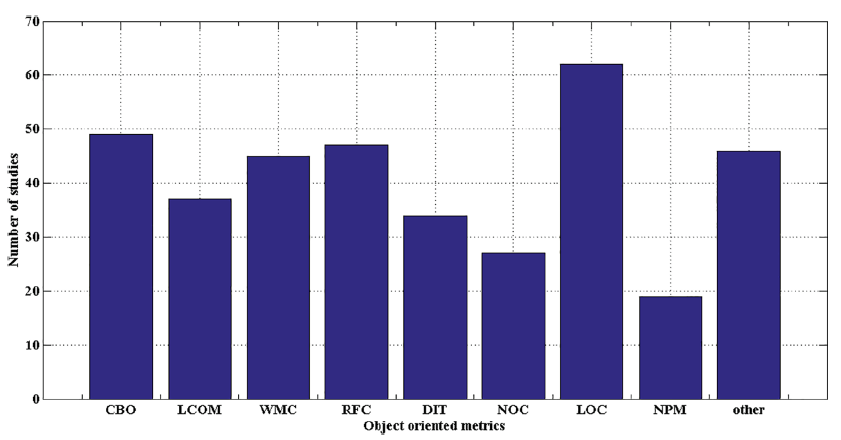
\includegraphics[width=\textwidth]{chapters/ChapterMarcoTeorico/sections/SoftwareMetrics/fig/oometrics.png}
    \setstretch{1} %Interlineado 1
	\captionsetup{labelsep=period, labelfont=bf}
    \caption{Lista de métricas de software orientado a objetos que son útiles para SFP. Tomado desde \cite{PANDEY2021114595}}
    \label{fig:OOmetrics}
\end{figure}
\section{Selección de características}

En \cite{9137899} combinan técnicas simples de eliminación de ruido, distribución desequilibrada de clases y selección de métricas de software para optimizar la predicción de defectos en software. La técnica fue probada en diez conjuntos de datos de predicción de fallos de software. Los resultados experimentales, incluyendo la recall, precisión, medida-F, exactitud y los valores de ROC-AUC, muestran que el método propuesto mejora el rendimiento de la predicción de fallos y los resultados obtenidos son mejores o cercanos a varios modelos comparativos. Se utilizan los conjuntos de datos NASA, Promise, y Github, combinando con los clasificadores: regresión logística, random forest (RF), SVM, naive Bayes.

\begin{figure}[H]
    \centering
    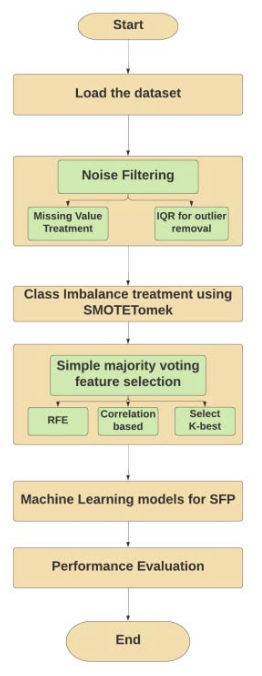
\includegraphics[]{chapters/ChapterMarcoTeorico/sections/FeaturesSelection/fig/Framework defining Methodology adopted for Software Defect.png}
    \setstretch{1} %Interlineado 1
	\captionsetup{labelsep=period, labelfont=bf}
    \caption{Marco que define la metodología adoptada para la predicción de defectos de software. Tomado desde \cite{9137899}}
    \label{fig:Frameworksd}
\end{figure}

En el paso de Selección de Características por Votación Mayoritaria Simple se utiliza un algoritmo de selección de atributos por votación mayoritaria simple para combinar el resultado de tres técnicas de selección de características, es decir, RFECV (eliminación recursiva de características con validación cruzada), selección de características basada en correlación y la técnica de seleccionar las k mejores.

En \cite{kondo2019impact} se utilizan tres Conjuntos de datos (PROMISE,NASA, AEEEM) sumando 26 proyectos en los que varian las metricas y la cantidad de registros.


\section{Datos Desbalanceados}

En la práctica, los modelos de predicción de defectos de software (SDP) a menudo sufren de datos muy desequilibrados, lo que dificulta a los clasificadores identificar instancias defectuosas. Recientemente, se propusieron muchas técnicas para abordar este problema; la técnica de sobremuestreo es uno de los métodos más conocidos para abordar el problema del desequilibrio de clases. Esta técnica equilibra el número de instancias defectuosas y no defectuosas generando nuevas instancias defectuosas.

Motivados por esto en \cite{8861051}, proponemos un enfoque de Sobremuestreo Basado en Clústeres con Filtrado de Ruido (KMFOS) para abordar el problema del desequilibrio de clases en SDP. KMFOS primero divide las instancias defectuosas en $K$ clústeres, y se generan nuevas instancias defectuosas por interpolación entre instancias de cada dos clústeres. Después de esto, estas nuevas instancias defectuosas se dispersarán diversamente en el espacio del conjunto de datos defectuoso. Luego, extendemos este sobremuestreo basado en clústeres mediante la Identificación de Ruido de Lista Cercana (CLNI) para limpiar las instancias de ruido. Realizamos experimentos extensivos en 24 proyectos para comparar KMFOS con algunos enfoques de sobremuestreo como SMOTE, BorderlineSMOTE, ADASYN, sobremuestreo aleatorio (ROS), SMOTE de K-medias, SMOTE + IPF, SMOTE + ENN y SMOTE + Enlaces de Tomek utilizando cinco clasificadores de predicción.
 

\begin{figure}[H]
    \centering
    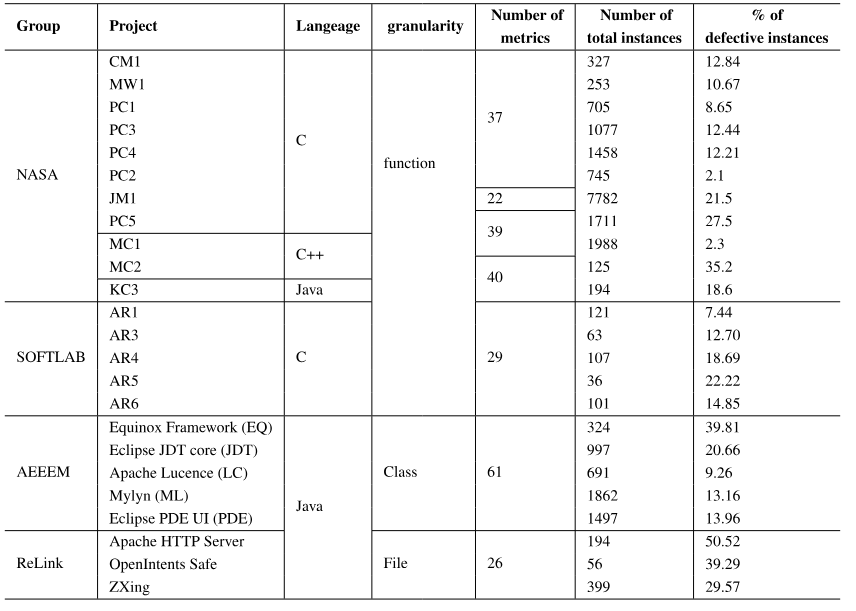
\includegraphics[width=\textwidth]{chapters/ChapterMarcoTeorico/sections/FeaturesSelection/fig/experimental dataset.png}
    \setstretch{1} %Interlineado 1
	\captionsetup{labelsep=period, labelfont=bf}
    \caption{Lista de datasets utilizados. Tomado desde \cite{8861051}}
    \label{fig:desequilibrioDataset}
\end{figure}

De la Figura \ref{fig:desequilibrioDataset}, podemos ver: i) los lenguajes de desarrollo de estos proyectos incluyen Java, C y C++; ii) la granularidad de las métricas cubre función, clase y archivo; iii) el número de instancias varía mucho y la proporción de instancias para la mayoría de los proyectos está muy por debajo del 25\%. Por lo tanto, estos proyectos pueden ser utilizados como objetos experimentales para evaluar estos enfoques con desequilibrio de clases.

En \cite{9044596} se utilizan los proyetos  cm1, kc1, mc2 y pc1 del repositorio PROMISE. Utilizan los clasificadores Logistic regression, NB, Decision tree, MNB y KNN combinados con las tecnicas de remuestreo SMOTE, ROS y RUS.
En la primera fase, aplican las técnicas de remuestreo para todos los clasificadores. En la segunda fase, la combinación de técnica de remuestreo y clasificador que ha tenido mejor desempeño se utiliza en el método de promediación de modelos. Esta combinación sobresaliente se obtiene a partir de las pruebas estadísticas. Su objetivo encontrar el conjunto sobresaliente de clasificador con técnica de remuestreo.




\section{Conjunto de datos}

Según la revisión de Pandey et al. \cite{PANDEY2021114595}, en la investigación sobre SFP se ha utilizado una gran variedad de conjuntos de datos. Su evidencia empírica muestra que el conjunto de datos de la NASA es el más aplicado en la disciplina, seguido de los conjuntos de datos de código abierto y del repositorio PROMISE.


\begin{figure}[H]
    \centering
    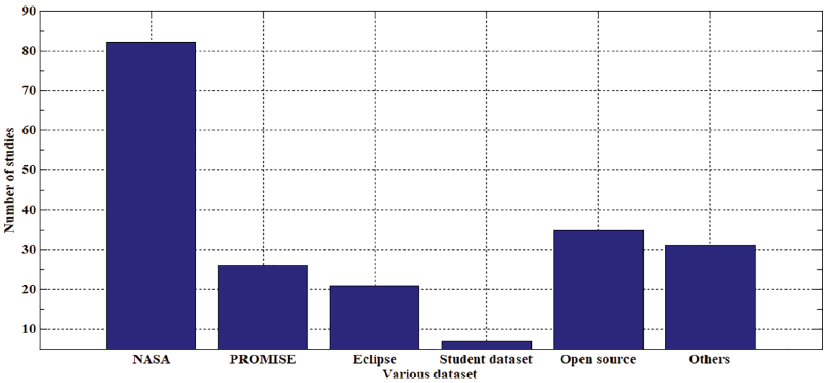
\includegraphics[width=\textwidth]{chapters/ChapterMarcoTeorico/sections/Datasets/fig/SFP dataset.png}
    \setstretch{1} %Interlineado 1
	\captionsetup{labelsep=period, labelfont=bf}
    \caption{Porcentaje de estudios para diferentes conjuntos de datos que se utilizan en SFP. \cite{PANDEY2021114595}}
    \label{fig:SFPDataset}
\end{figure}

Se pueden encontrar algunos patrones en la Figura \ref{fig:datasetdist} en que el conjunto de datos con la distribución de fallos más baja es popularmente utilizado y viceversa. Según el gráfico de barras, los conjuntos de datos de la NASA tienen menos distribución de fallos (CM1, PC1, KC3, MW1, PC4) en comparación con el conjunto de datos del repositorio PROMISE (poi-3.0, lucene-2.4, eclipse-3.0, eclipse-2.1). Una información adicional que informa esta figura es que, en algunos casos, los conjuntos de datos que tienen un gran número de instancias tienen menos distribución de fallos, como JM1. CM1 y JM1 también son conjuntos de datos sustancialmente utilizados que combinan el 57\% de los estudios y contienen el 31\% de los módulos defectuosos.

\begin{figure}[H]
    \centering
    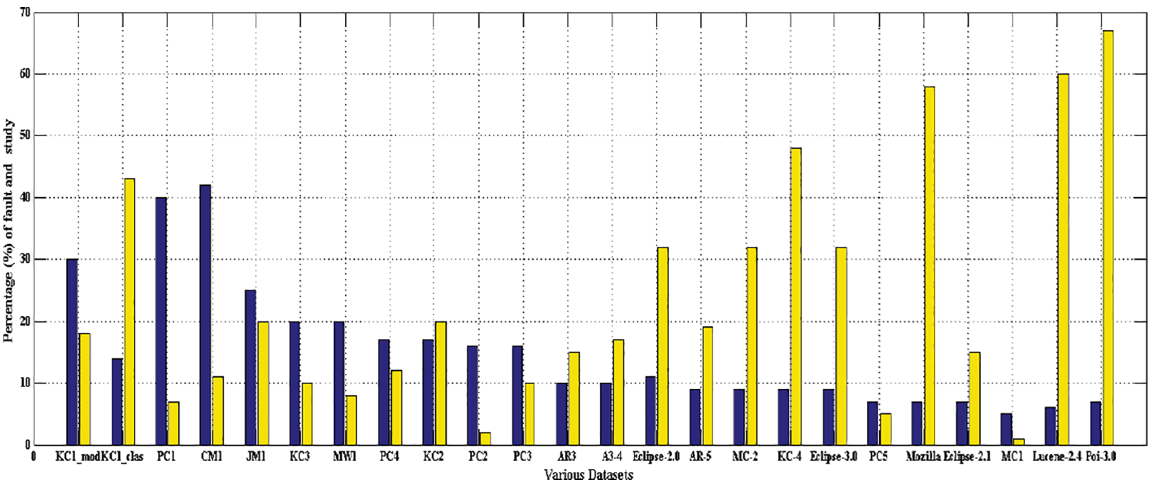
\includegraphics[width=\textwidth]{chapters/ChapterMarcoTeorico/sections/Datasets/fig/datasetdist.png}
    \setstretch{1} %Interlineado 1
	\captionsetup{labelsep=period, labelfont=bf}
    \caption{Distribución de errores de diferentes conjuntos de datos. \cite{PANDEY2021114595}}
    \label{fig:datasetdist}
\end{figure}

\section{Algoritmos utilizados en SFP}
\label{sec:clasificadores_mt}

La predicción de fallas de software (SFP) es una tarea crítica en la ingeniería de software que busca identificar los módulos del software que son propensos a contener defectos. Para realizar esta predicción, se han utilizado varios algoritmos de aprendizaje automático y técnicas estadísticas. A continuación, se describen algunos de los algoritmos más comúnmente utilizados en la literatura para SFP.

\subsubsection{Regresión Logística}
La regresión logística es un método estadístico utilizado para modelar la probabilidad de que una instancia pertenezca a una de dos clases posibles. Este método ha sido ampliamente utilizado en SFP debido a su simplicidad y efectividad para manejar datos binarios. La regresión logística estima la relación entre las variables independientes (métricas del software) y la variable dependiente (presencia o ausencia de defectos) mediante una función logística \cite{kondo2019impact}.

\subsubsection{Máquinas de Vectores de Soporte (SVM)}
Las máquinas de vectores de soporte (SVM) son un conjunto de métodos de aprendizaje supervisado utilizados para clasificación y regresión. Una SVM busca el hiperplano que separa las dos clases con el máximo margen, es decir, con la mayor distancia posible a las instancias más cercanas de cada clase (los vectores de soporte); la formulación de margen suave permite tolerar instancias mal clasificadas mediante un parámetro de penalización \cite{cortes1995}. En su versión lineal, la SVM es rápida de entrenar sobre conjuntos grandes y sensible a la escala de las características, por lo que requiere estandarizarlas previamente. En el contexto de SFP, la SVM ha demostrado ser eficaz para manejar conjuntos de datos de alta dimensionalidad. En esta tesis se utiliza una SVM lineal con estandarización previa como uno de los clasificadores del análisis de sensibilidad.

\subsubsection{Árboles de Decisión}
Los árboles de decisión son modelos de predicción que utilizan un árbol como estructura de decisión y modelan la relación entre las variables de entrada y la variable de salida. Los árboles de decisión, como el algoritmo J48, han sido utilizados en SFP debido a su capacidad para manejar datos categóricos y continuos, y su facilidad de interpretación \cite{RADJENOVIC20131397}.

\subsubsection{Random Forest}
El algoritmo Random Forest \cite{breiman2001} es un conjunto de árboles de decisión, cada uno entrenado sobre una muestra \textit{bootstrap} de las instancias (\textit{bagging}) y considerando en cada división solo un subconjunto aleatorio de las características. La predicción final se obtiene por votación mayoritaria de los árboles. La combinación de ambas fuentes de aleatoriedad reduce la correlación entre árboles y, con ello, la varianza y el riesgo de sobreajuste del modelo \cite{shah_comparative_2020}. Random Forest es uno de los clasificadores más utilizados en SFP y es el clasificador principal de esta tesis, empleado tanto en Weka \cite{weka} como en \textit{scikit-learn}.

\subsubsection{XGBoost}
XGBoost \cite{chen2016} es una implementación escalable del \textit{boosting} de gradiente sobre árboles de decisión. A diferencia de Random Forest, que entrena árboles independientes y promedia sus votos, el \textit{boosting} construye los árboles de forma secuencial: cada nuevo árbol se ajusta para corregir los errores residuales del conjunto acumulado, minimizando una función de pérdida mediante descenso de gradiente con regularización explícita de la complejidad de los árboles. XGBoost representa, por tanto, un paradigma de ensamble distinto al de Random Forest, y se utiliza en el análisis de sensibilidad de esta tesis para verificar que los hallazgos no son específicos de un único clasificador.

\subsubsection{Naive Bayes}
Naive Bayes es un clasificador basado en la teoría de probabilidad bayesiana. Asume la independencia entre las características, lo cual es una simplificación fuerte pero efectiva en muchos casos. En SFP, Naive Bayes ha sido utilizado debido a su simplicidad y eficiencia computacional, especialmente cuando se dispone de grandes conjuntos de datos con múltiples características.

\subsubsection{K-Nearest Neighbors (KNN)}
El algoritmo K-Nearest Neighbors (KNN) es un método de clasificación que asigna una clase a una instancia basándose en las clases de sus k vecinos más cercanos en el espacio de características. KNN ha sido aplicado en SFP debido a su simplicidad y efectividad para capturar relaciones locales en los datos. Sin embargo, puede ser computacionalmente costoso cuando se trabaja con grandes conjuntos de datos.

\subsubsection{Algoritmos de Sobremuestreo y Submuestreo}
Para abordar el problema del desequilibrio de clases en los conjuntos de datos de SFP, se utilizan técnicas de sobremuestreo y submuestreo. Métodos como SMOTE (Synthetic Minority Over-sampling Technique), ROS (Random Over-Sampling), y RUS (Random Under-Sampling) se emplean para equilibrar las clases defectuosas y no defectuosas, con el objetivo de reducir el sesgo del clasificador hacia la clase mayoritaria \cite{9137899,chawla2002}. Su efecto real, sin embargo, depende del contexto experimental y de la métrica de evaluación \cite{8494821}, un aspecto central de esta tesis.

\subsubsection{Modelos de Conjunto}
Los modelos de conjunto, como el Bagging y el Boosting, combinan múltiples clasificadores para mejorar la precisión y la robustez del modelo. Estas técnicas son útiles en SFP para combinar las predicciones de diferentes algoritmos y obtener una mejor estimación de la propensión a fallos de los módulos de software \cite{9044596}.

En resumen, una variedad de algoritmos de aprendizaje automático y técnicas de preprocesamiento se utilizan en la predicción de fallas de software, cada uno con sus propias ventajas y limitaciones. La selección del algoritmo adecuado depende de las características específicas del conjunto de datos y del problema en cuestión.



%..................................	
	\chapter{\MakeUppercase{Materiales y métodos}} \label{cap3}
	En este capítulo se presenta una descripción detallada del conjunto de datos BugHunter, incluyendo su origen, estructura, y una descripción exhaustiva de sus características (métricas de código) y tamaño. Se detallan las herramientas y técnicas empleadas, así como las distintas etapas del proceso de selección de características. Finalmente, se describe el procedimiento adoptado para llevar a cabo los experimentos, incluyendo los pasos seguidos para entrenar y validar los modelos.

\section{BUGHUNTER}


Utilizamos el Conjunto de datos BugHunter: un tipo novedoso de conjunto de datos de errores construido automáticamente y disponible gratuitamente que contiene elementos de código (archivos, clases, métodos) con un amplio conjunto de métricas de código e información de errores \cite{ferenc_automatically_2020}.

Otros conjuntos de datos de errores disponibles siguen el enfoque tradicional (PROMISE \cite{sayyad_shirabad_promise_2005}, Eclipse, entre otros) de recopilar las características de todos los elementos del código fuente (con errores y sin errores) en solo una o más versiones de lanzamiento preseleccionadas del código. El enfoque seleccionado, por otro lado, captura el error y los estados fijos de los mismos elementos del código fuente desde el marco de tiempo más estrecho que podemos identificar para detectar la presencia de un error, independientemente de las versiones de lanzamiento.

El conjunto de datos contiene información útil de caracterización de elementos de código defectuoso, se utilizan varios proyectos almacenados en GitHub que son mantenidos regularmente. Se utiliza la API de GitHub que hace posible implementar una herramienta de recuperación automática de datos. Se seleccionan 15 proyectos Java como sistemas temáticos, que difieren en muchos aspectos entre sí (tamaño, dominio, número de errores informados) para cubrir un conjunto amplio y general de sistemas \cite{ferenc_automatically_2020}. 

El conjunto de datos se basa en un nuevo enfoque que recopila información del instante antes y después de la corrección de los elementos del código fuente (y sus características) que se vieron afectados por errores y no considera aquellos elementos del código que no fueron afectados por errores. Este tipo de conjunto de datos ayuda a capturar los cambios en las métricas de los productos de software cuando se corrige un error. Por lo tanto, se puede aprender de las diferencias en las métricas del código fuente entre elementos de código defectuosos y no defectuosos.

En la tabla \ref{table:datasetmeta}, resumimos los metadatos principales del conjunto de datos. La cantidad de métricas existentes en cada categoría y la cantidad de registros existentes en cada uno de los niveles de granularidad.

\begin{table}[H]
\captionsetup{labelsep=period, labelfont=bf}
\caption{Metadatos del conjunto de datos}
\centering
\begin{tabular}{lc}
\toprule
\textbf{Granularity}        & file, class, method                                                                                                                \\\midrule
\textbf{Number of projects} & 15                                                                                                                                 \\ 
\hline
\textbf{Number of metrics}  & \begin{tabular}[c]{@{}c@{}}static source code metrics (66),\\ code duplication metrics (8),\\ code smell metrics (35)\end{tabular} \\
\hline
\textbf{Number of entries}  & \begin{tabular}[c]{@{}c@{}}file: 70,088\\ class: 84,562\\ method: 159,078


\end{tabular}  
\\\bottomrule
\end{tabular}

\label{table:datasetmeta}
\end{table} 

 Realizamos una descripción de los datos en \ref{description-table} mostrando cantidad, media, desviación estándar, mínimo, máximo y cantidad de elementos. Al analizar la tabla descriptiva de los datos podemos concluir:
 {
\fontsize{14pt}{14pt}\selectfont
\begin{itemize}
\item No existen datos nulos dado que el contados de todos es igual al total de registros.
\item Gran variedad en los rangos de los datos.
\item Una gran cantidad de características que tienen moda y mediana iguales y con valor 0, pudiendo implicar poca variación en sus datos.
\end{itemize}
}

El conjunto de datos BugHunter cuenta con varias métricas de código extraídas con la herramienta OpenStaticAnalyzer \cite{openstaticanalyzergithubio} utilizando el código etiquetado en el GitHub de 15 proyectos, escritos en Java. Especialmente los más grandes y que tengan una cantidad adecuada de problemas etiquetados como errores, porque son más adecuados para este tipo de análisis.

\begin{table}[H]
{
\captionsetup{labelsep=period, labelfont=bf}
\caption{ Description Table}
\fontsize{9pt}{6pt}\selectfont
\begin{tabular}{@{}lp{10mm}p{10mm}p{10mm}p{10mm}llllll@{}} 
\toprule
Medida& Media & Error   típico & Mediana & Moda & Desviación   estándar & Varianza   de la muestra & Mínimo & Máximo & Suma& Cuenta \\ 
\midrule
CC                                  & 0,12           & 0,00                    & 0,00             & 0,00          & 0,30                           & 0,09                              & 0,00            & 1,00            & 19334,08       & 159078,00       \\
CCL                                 & 0,66           & 0,03                    & 0,00             & 0,00          & 11,53                          & 133,02                            & 0,00            & 499,00          & 104713,00      & 159078,00       \\
CCO                                 & 4,01           & 0,71                    & 0,00             & 0,00          & 282,97                         & 80069,76                          & 0,00            & 75248,00        & 638669,00      & 159078,00       \\
CI                                  & 1,95           & 0,14                    & 0,00             & 0,00          & 56,22                          & 3160,84                           & 0,00            & 4671,00         & 310335,00      & 159078,00       \\
CLC                                 & 0,12           & 0,00                    & 0,00             & 0,00          & 0,30                           & 0,09                              & 0,00            & 1,00            & 19071,79       & 159078,00       \\
LDC                                 & 7,52           & 0,37                    & 0,00             & 0,00          & 146,09                         & 21343,22                          & 0,00            & 6691,00         & 1196598,00     & 159078,00       \\
LLDC                                & 6,72           & 0,33                    & 0,00             & 0,00          & 132,41                         & 17531,44                          & 0,00            & 5848,00         & 1068422,00     & 159078,00       \\
HCPL                                & 202,83         & 1,94                    & 106,09           & 13,61         & 771,92                         & 595862,35                         & 2,00            & 57839,10        & 32266128,82    & 159078,00       \\
HDIF                                & 26,30          & 0,96                    & 15,04            & 3,50          & 384,17                         & 147587,63                         & 1,00            & 56556,50        & 4183142,22     & 159078,00       \\
HEFF                                & 250671,02      & 65265,39                & 3554,80          & 49,13         & 26030828,33                    & 677604023793090,00                & 4,75            & 3944690000,00   & 39876245063,67 & 159078,00       \\
HNDB                                & 910,90         & 43,12                   & 232,92           & 13,41         & 17198,86                       & 295800753,28                      & 2,83            & 2496560,00      & 144904764,53   & 159078,00       \\
HPL                                 & 120,57         & 2,12                    & 48,00            & 12,00         & 844,70                         & 713519,30                         & 3,00            & 39378,00        & 19180331,00    & 159078,00       \\
HPV                                 & 39,73          & 0,19                    & 27,00            & 10,00         & 74,43                          & 5539,97                           & 3,00            & 4764,00         & 6319883,00     & 159078,00       \\
HTRP                                & 13926,17       & 3625,86                 & 197,49           & 2,73          & 1446157,65                     & 2091371943879,64                  & 0,26            & 219150000,00    & 2215347324,87  & 159078,00       \\
HVOL                                & 848,92         & 23,68                   & 230,00           & 19,65         & 9444,64                        & 89201173,08                       & 4,75            & 451128,00       & 135044408,26   & 159078,00       \\
MI                                  & 104,36         & 0,06                    & 106,10           & 132,83        & 23,81                          & 567,01                            & -579,07         & 162,66          & 16602174,03    & 159078,00       \\
MIMS                                & 61,05          & 0,03                    & 62,05            & 77,68         & 13,74                          & 188,78                            & 0,00            & 95,12           & 9712500,44     & 159078,00       \\
MISEI                               & 83,11          & 0,08                    & 84,46            & 116,03        & 33,76                          & 1139,90                           & -668,08         & 208,70          & 13221672,48    & 159078,00       \\
MISM                                & 48,73          & 0,05                    & 49,39            & 67,85         & 19,25                          & 370,44                            & 0,00            & 122,05          & 7751585,71     & 159078,00       \\
McCC                                & 3,54           & 0,03                    & 1,00             & 1,00          & 12,08                          & 146,02                            & 1,00            & 2387,00         & 562498,00      & 159078,00       \\
NL                                  & 1,08           & 0,01                    & 0,00             & 0,00          & 2,03                           & 4,12                              & 0,00            & 82,00           & 171181,00      & 159078,00       \\
NLE                                 & 0,94           & 0,00                    & 0,00             & 0,00          & 1,35                           & 1,82                              & 0,00            & 27,00           & 150219,00      & 159078,00       \\
NII                                 & 1,60           & 0,03                    & 0,00             & 0,00          & 13,08                          & 171,14                            & 0,00            & 1833,00         & 253982,00      & 159078,00       \\
NOI                                 & 5,79           & 0,02                    & 3,00             & 1,00          & 8,50                           & 72,30                             & 0,00            & 185,00          & 920814,00      & 159078,00       \\
CD                                  & 0,05           & 0,00                    & 0,00             & 0,00          & 0,13                           & 0,02                              & 0,00            & 0,95            & 8743,04        & 159078,00       \\
CLOC                                & 1,35           & 0,01                    & 0,00             & 0,00          & 3,81                           & 14,53                             & 0,00            & 198,00          & 214253,00      & 159078,00       \\
DLOC                                & 0,54           & 0,01                    & 0,00             & 0,00          & 2,39                           & 5,70                              & 0,00            & 195,00          & 86694,00       & 159078,00       \\
TCD                                 & 0,05           & 0,00                    & 0,00             & 0,00          & 0,13                           & 0,02                              & 0,00            & 0,95            & 8603,51        & 159078,00       \\
TCLOC                               & 1,40           & 0,01                    & 0,00             & 0,00          & 3,92                           & 15,36                             & 0,00            & 198,00          & 222238,00      & 159078,00       \\
LLOC                                & 19,96          & 0,32                    & 9,00             & 4,00          & 127,48                         & 16250,40                          & 1,00            & 5851,00         & 3175814,00     & 159078,00       \\
LOC                                 & 22,73          & 0,35                    & 10,00            & 4,00          & 141,47                         & 20015,14                          & 1,00            & 6273,00         & 3615214,00     & 159078,00       \\
NOS                                 & 13,33          & 0,27                    & 5,00             & 1,00          & 106,34                         & 11308,68                          & 0,00            & 5079,00         & 2120731,00     & 159078,00       \\
NUMPAR                              & 1,14           & 0,00                    & 1,00             & 0,00          & 1,60                           & 2,56                              & 0,00            & 38,00           & 180569,00      & 159078,00       \\
TLLOC                               & 21,51          & 0,34                    & 10,00            & 4,00          & 134,48                         & 18085,43                          & 1,00            & 5851,00         & 3421101,00     & 159078,00       \\
TLOC                                & 24,43          & 0,37                    & 11,00            & 4,00          & 148,75                         & 22125,86                          & 1,00            & 6703,00         & 3885847,00     & 159078,00       \\
TNOS                                & 14,01          & 0,27                    & 5,00             & 1,00          & 108,60                         & 11794,42                          & 0,00            & 5079,00         & 2229242,00     & 159078,00       \\
WarningBlocker                      & 0,00           & 0,00                    & 0,00             & 0,00          & 0,00                           & 0,00                              & 0,00            & 1,00            & 1,00           & 159078,00       \\
WarningCritical                     & 0,11           & 0,00                    & 0,00             & 0,00          & 0,81                           & 0,66                              & 0,00            & 45,00           & 17572,00       & 159078,00       \\
WarningInfo                         & 0,00           & 0,00                    & 0,00             & 0,00          & 0,00                           & 0,00                              & 0,00            & 0,00            & 0,00           & 159078,00       \\
WarningMajor                        & 0,49           & 0,00                    & 0,00             & 0,00          & 1,80                           & 3,26                              & 0,00            & 79,00           & 78578,00       & 159078,00       \\
WarningMinor                        & 2,32           & 0,10                    & 0,00             & 0,00          & 39,21                          & 1537,67                           & 0,00            & 2889,00         & 368755,00      & 159078,00       \\
Android Rules                       & 0,00           & 0,00                    & 0,00             & 0,00          & 0,00                           & 0,00                              & 0,00            & 0,00            & 0,00           & 159078,00       \\
Basic Rules                         & 0,05           & 0,00                    & 0,00             & 0,00          & 0,42                           & 0,18                              & 0,00            & 34,00           & 7199,00        & 159078,00       \\
Brace Rules                         & 0,35           & 0,02                    & 0,00             & 0,00          & 9,89                           & 97,87                             & 0,00            & 2290,00         & 55578,00       & 159078,00       \\
Clone Implementation Rules          & 0,00           & 0,00                    & 0,00             & 0,00          & 0,02                           & 0,00                              & 0,00            & 2,00            & 55,00          & 159078,00       \\
Code Size Rules                     & 0,00           & 0,00                    & 0,00             & 0,00          & 0,00                           & 0,00                              & 0,00            & 0,00            & 0,00           & 159078,00       \\
Comment Rules                       & 0,00           & 0,00                    & 0,00             & 0,00          & 0,00                           & 0,00                              & 0,00            & 0,00            & 0,00           & 159078,00       \\
Controversial Rules                 & 0,06           & 0,00                    & 0,00             & 0,00          & 0,26                           & 0,07                              & 0,00            & 11,00           & 10096,00       & 159078,00       \\
Coupling Rules                      & 0,00           & 0,00                    & 0,00             & 0,00          & 0,00                           & 0,00                              & 0,00            & 0,00            & 0,00           & 159078,00       \\
Design Rules                        & 1,41           & 0,09                    & 0,00             & 0,00          & 36,77                          & 1351,85                           & 0,00            & 2807,00         & 224629,00      & 159078,00       \\
Empty Code Rules                    & 0,02           & 0,00                    & 0,00             & 0,00          & 0,25                           & 0,06                              & 0,00            & 34,00           & 2414,00        & 159078,00       \\
Finalizer Rules                     & 0,00           & 0,00                    & 0,00             & 0,00          & 0,01                           & 0,00                              & 0,00            & 1,00            & 24,00          & 159078,00       \\
Import Statement Rules              & 0,06           & 0,00                    & 0,00             & 0,00          & 1,48                           & 2,19                              & 0,00            & 81,00           & 9044,00        & 159078,00       \\
J2EE Rules                          & 0,00           & 0,00                    & 0,00             & 0,00          & 0,04                           & 0,00                              & 0,00            & 5,00            & 132,00         & 159078,00       \\
JUnit Rules                         & 0,43           & 0,01                    & 0,00             & 0,00          & 2,02                           & 4,07                              & 0,00            & 150,00          & 68963,00       & 159078,00       \\
Jakarta Commons Logging Rules       & 0,01           & 0,00                    & 0,00             & 0,00          & 0,18                           & 0,03                              & 0,00            & 9,00            & 2056,00        & 159078,00       \\
Java Logging Rules                  & 0,04           & 0,00                    & 0,00             & 0,00          & 0,39                           & 0,15                              & 0,00            & 46,00           & 6637,00        & 159078,00       \\
JavaBean Rules                      & 0,00           & 0,00                    & 0,00             & 0,00          & 0,00                           & 0,00                              & 0,00            & 0,00            & 0,00           & 159078,00       \\
MigratingToJUnit4 Rules             & 0,00           & 0,00                    & 0,00             & 0,00          & 0,00                           & 0,00                              & 0,00            & 0,00            & 0,00           & 159078,00       \\
Migration Rules                     & 0,00           & 0,00                    & 0,00             & 0,00          & 0,04                           & 0,00                              & 0,00            & 6,00            & 124,00         & 159078,00       \\
Migration13 Rules                   & 0,00           & 0,00                    & 0,00             & 0,00          & 0,00                           & 0,00                              & 0,00            & 0,00            & 0,00           & 159078,00       \\
Migration14 Rules                   & 0,00           & 0,00                    & 0,00             & 0,00          & 0,00                           & 0,00                              & 0,00            & 0,00            & 0,00           & 159078,00       \\
Migration15 Rules                   & 0,00           & 0,00                    & 0,00             & 0,00          & 0,00                           & 0,00                              & 0,00            & 0,00            & 0,00           & 159078,00       \\
Naming Rules                        & 0,05           & 0,00                    & 0,00             & 0,00          & 0,25                           & 0,06                              & 0,00            & 8,00            & 8554,00        & 159078,00       \\
Optimization Rules                  & 0,01           & 0,00                    & 0,00             & 0,00          & 0,16                           & 0,02                              & 0,00            & 15,00           & 1787,00        & 159078,00       \\
Security Code Guideline Rules       & 0,00           & 0,00                    & 0,00             & 0,00          & 0,06                           & 0,00                              & 0,00            & 3,00            & 552,00         & 159078,00       \\
Strict Exception Rules              & 0,11           & 0,00                    & 0,00             & 0,00          & 0,44                           & 0,19                              & 0,00            & 14,00           & 17806,00       & 159078,00       \\
String and StringBuffer Rules       & 0,11           & 0,00                    & 0,00             & 0,00          & 0,97                           & 0,94                              & 0,00            & 88,00           & 17568,00       & 159078,00       \\
Type Resolution Rules               & 0,16           & 0,00                    & 0,00             & 0,00          & 0,41                           & 0,17                              & 0,00            & 11,00           & 24819,00       & 159078,00       \\
Unnecessary and   Unused Code Rules & 0,06           & 0,00                    & 0,00             & 0,00          & 1,45                           & 2,11                              & 0,00            & 79,00           & 9382,00        & 159078,00       \\
Vulnerability Rules                 & 0,00           & 0,00                    & 0,00             & 0,00          & 0,00                           & 0,00                              & 0,00            & 1,00            & 1,00           & 159078,00       \\
Number of Bugs                      & 0,47           & 0,00                    & 0,00             & 0,00          & 0,70                           & 0,50                              & 0,00            & 6,00            & 75096,00       & 159078,00       \\ 
\bottomrule
\end{tabular}
\label{description-table}
}
\end{table}











En la \ref{metrics-table} se muestra al conjunto de métricas y sus niveles correspondientes, el BugHunter contiene las métricas de código en tres niveles (método, clase y archivo).

\begin{table}[H]
{
\fontsize{8pt}{4pt}\selectfont
\captionsetup{labelsep=period, labelfont=bf}
\caption{Métricas del código fuente}
\centering
\begin{tabular}{lllll}
\toprule
Abreviación & Nombre Completo                               & Método & Clase & Archivo \\
\midrule
CLOC        & Comment Lines of Code                         & X      & X     & X       \\
LOC         & Lines of Code                                 & X      & X     & X       \\
LLOC        & Logical Lines of Code                         & X      & X     & X       \\
NL          & Nesting Level                                 & X      & X     &         \\
NLE         & Nesting Level Else-If                         & X      & X     &         \\
NII         & Number of Incoming   Invocations              & X      & X     &         \\
NOI         & Number of Outgoing Invocations                & X      & X     &         \\
CD          & Comment Density                               & X      & X     &         \\
DLOC        & Documentation Lines of Code                   & X      & X     &         \\
TCD         & Total Comment Density                         & X      & X     &         \\
TCLOC       & Total Comment   Lines of Code                 & X      & X     &         \\
NOS         & Number of Statements                          & X      & X     &         \\
TLOC        & Total Lines of Code                           & X      & X     &         \\
TLLOC       & Total   Logical Lines of Code                 & X      & X     &         \\
TNOS        & Total Number of Statements                    & X      & X     &         \\
McCC        & McCabe’s Cyclomatic Comple   ity              & X      &       & X       \\
PDA         & Public Documented API                         &        & X     & X       \\
PUA         & Public Undocumented API                       &        & X     & X       \\
HCPL        & Halstead Calculated Program Length            & X      &       &         \\
HDIF        & Halstead Difficulty                           & X      &       &         \\
HEFF        & Halstead Effort                               & X      &       &         \\
HNDB        & Halstead   Number of Delivered Bugs           & X      &       &         \\
HPL         & Halstead Program Length                       & X      &       &         \\
HPV         & Halstead Program   Vocabulary                 & X      &       &         \\
HTRP        & Halstead Time   Required to Program           & X      &       &         \\
HVOL        & Halstead Volume                               & X      &       &         \\
MIMS        & Maintainability Index (Microsoft version)     & X      &       &         \\
MI          & Maintainability Index   (Original version)    & X      &       &         \\
MISEI       & Maintainability Index (SEI version)           & X      &       &         \\
MISM        & Maintainability Index   (SourceMeter version) & X      &       &         \\
NUMPAR      & Number of Parameters                          & X      &       &         \\
LCOM5       & Lack   of Cohesion in Methods                 &        & X     &         \\
WMC         & Weighted Methods per Class                    &        & X     &         \\
CBO         & Coupling Between Object   classes             &        & X     &         \\
CBOI        & Coupling Between   Object classes Inverse     &        & X     &         \\
RFC         & Response set For Class                        &        & X     &         \\
AD          & API Documentation                             &        & X     &         \\
DIT         & Depth of Inheritance   Tree                   &        & X     &         \\
NOA         & Number of Ancestors                           &        & X     &         \\
NOC         & Number of Children                            &        & X     &         \\
NOD         & Number of Descendants                         &        & X     &         \\
NOP         & Number of Parents                             &        & X     &         \\
NA          & Number of Attributes                          &        & X     &         \\
NG          & Number of Getters                             &        & X     &         \\
NLA         & Number of Local Attributes                    &        & X     &         \\
NLG         & Number of Local Getters                       &        & X     &         \\
NLM         & Number of Local Methods                       &        & X     &         \\
NLPA        & Number   of Local Public Attributes           &        & X     &         \\
NLPM        & Number of Local   Public Methods              &        & X     &         \\
NLS         & Number of Local Setters                       &        & X     &         \\
NM          & Number of Methods                             &        & X     &         \\
NPA         & Number of Public   Attributes                 &        & X     &         \\
NPM         & Number of Public Methods                      &        & X     &         \\
NS          & Number of Setters                             &        & X     &         \\
TNA         & Total Number of Attributes                    &        & X     &         \\
TNG         & Total Number of Getters                       &        & X     &         \\
TNLA        & Total Number of   Local Attributes            &        & X     &         \\
TNLG        & Total   Number of Local Getters               &        & X     &         \\
TNLM        & Total Number of   Local Methods               &        & X     &         \\
TNLPA       & Total   Number of Local Public Attributes     &        & X     &         \\
TNLPM       & Total Number of   Local Public Methods        &        & X     &         \\
TNLS        & Total   Number of Local Setters               &        & X     &         \\
TNM         & Total Number of Methods                       &        & X     &         \\
TNPA        & Total   Number of Public Attributes           &        & X     &         \\
TNPM        & Total Number of   Public Methods              &        & X     &         \\
TNS         & Total Number of Setters                       &        & X     &        \\
\bottomrule
\end{tabular}

\label{metrics-table}
}
\end{table}


OpenStaticAnalyzer también proporciona un módulo de detección de violaciones de reglas de codificación mostradas en la tabla \ref{table:smell_metrics}. La presencia de violaciones de reglas en un elemento de código fuente puede causar errores en una fase posterior, por lo tanto, la cantidad de violaciones de reglas diferentes ubicadas en un elemento del código fuente puede servir como predictores y el conjunto de datos también encapsula esta información. 


\begin{table}[H]
{
\fontsize{9pt}{5pt}\selectfont
\captionsetup{labelsep=period, labelfont=bf}
\caption{Métricas de violación de reglas}
\centering
\begin{tabular}{ll}
 \toprule
\textbf{Abreviación} & \textbf{Nombre completo}          \\
\midrule
WI                   & WarningInfo                                           \\
WMA                  & WarningMajor                                         \\
AR                   & Android Rules                                          \\
BAR                  & Basic Rules                                            \\
CSR                  & Controversial Rules                                    \\
CR                   & Coupling Rules                                        \\
NR                   & Naming Rules                                           \\
OR                   & Optimization Rules                                     \\
SCGR                 & Security Code Guideline Rules                          \\
SER                  & Strict Exception Rules                                 \\
SSR                  & String and StringBuffer Rules                           \\
TRR                  & Type Resolution Rules                                  \\
VR                   & Vulnerability Rules                                   \\
J2EER                & J2EE Rules                                              \\
WC                   & WarningCritical                                          \\
UUCR                 & Unnecessary and Unused Code Rules                         \\
JLR                  & Java Logging Rules                                       \\
ISR                  & Import Statement Rules                                    \\
M15R                 & Migration15 Rules                                         \\
WMI                  & WarningMinor                                              \\
MR                   & Migration Rules                                           \\
M13R                 & Migration13 Rules                                         \\
M14R                 & Migration14 Rules                                        \\
MUR                  & MigratingToJUnit4 Rules                                   \\
JBR                  & JavaBean Rules                                            \\
JCLR                 & Jakarta Commons Logging Rules                             \\
JUR                  & JUnit Rules                                              \\
FR                   & Finalizer Rules                                           \\
ECR                  & Empty Code Rules                                          \\
DR                   & Design Rules                                              \\
CR                   & Comment Rules                                             \\
CIR                  & Clone Implementation Rules                               \\
BRR                  & Brace Rules   \\
\bottomrule
\end{tabular}

\label{table:smell_metrics}
}
\end{table}

\section{Preprocesamiento de datos en dos etapas}\label{sec:segunda}

En este artículo se utiliza un enfoque novedoso de preprocesamiento de datos en dos etapas que incorpora tanto la selección de características como la reducción de instancias propuesto en \cite{liu_empirical_2015}. Específicamente, en la etapa de selección de características, primero realizamos un análisis de relevancia y luego proponemos un método de agrupamiento basado en umbrales, llamado algoritmo de agrupamiento basado en umbrales, para realizar el control de redundancia. En la etapa de reducción de instancias, aplicamos submuestreo aleatorio para mantener el equilibrio entre las instancias defectuosas y no defectuosas.

\subsection{Etapa de selección de características}

El primer paso es realizar un análisis de relevancia para eliminar las características irrelevantes y el segundo paso es realizar un control de redundancia para eliminar las características redundantes. 

\begin{figure}[h!]
    \centering
    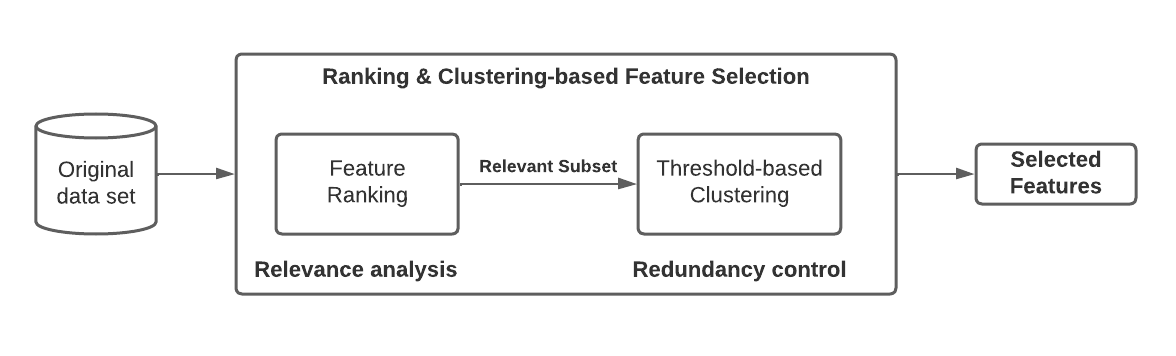
\includegraphics[width=\textwidth]{figs/etapas/Imagen1.png}
    \setstretch{1} %Interlineado 1
	\captionsetup{labelsep=period, labelfont=bf}
    \caption{Detalle de los pasos del modelo de selección}
    \label{fig:logos}
\end{figure}

\subsubsection{Análisis de relevancia}

En el proceso de clasificación, la relevancia de las características individuales se evalúa en el primer paso. Este análisis implica clasificar las características según su importancia o pesos, que son cruciales para diferenciar instancias entre diversas clases (por ejemplo, Bug o NoBug). Para este propósito, se adopta una representación específica de cada grupo, como se describe en \cite{chen_empirical_2013}.



\begin{itemize}
\item Ganancia de información (IG): La idea detrás de este algoritmo es que las características que proporcionan la mayor ganancia de información son las más útiles para la tarea de clasificación o predicción que estamos realizando.

La fórmula matemática para calcular la ganancia de información es la siguiente:

Ganancia de información = Entropía inicial - Entropía final

Donde la entropía inicial es la entropía del conjunto de datos antes de utilizar la característica para dividir el conjunto en subconjuntos más pequeños, y la entropía final es la suma de las entropías de cada subconjunto después de dividir el conjunto de datos utilizando la característica.

La entropía se calcula utilizando la siguiente fórmula:
\begin{equation}
\text{Entropía} = - \sum_{x} p(x) \log_{2}\left(p(x)\right)
	\label{eq:entropia}
\end{equation}

Donde p(x) es la probabilidad de que una observación pertenezca a la clase x.

\item Chi-Cuadrado (CS): El algoritmo Chi-Cuadrado es una técnica estadística utilizada para evaluar si existe una relación entre dos variables categóricas.

 Para calcular el valor Chi-Cuadrado, comparamos la distribución esperada con la distribución observada, es decir, con los valores reales de cada combinación de valores de A y B en nuestro conjunto de datos. Si la diferencia entre la distribución esperada y la observada es significativamente grande, podemos concluir que existe una relación entre las dos variables.

La fórmula para calcular el valor Chi-Cuadrado es la siguiente:
\begin{equation}
\text{Chi-Cuadrado} = \sum \frac{(O - E)^{2}}{E}
	\label{eq:chisqr}
\end{equation}

\item ReliefF (RF): A diferencia de otros algoritmos de selección de características, como la ganancia de información o el algoritmo Chi-Cuadrado, ReliefF tiene en cuenta la relación entre las características y las etiquetas o clases en el conjunto de datos.

El algoritmo ReliefF utiliza la distancia para evaluar cuánto aporta cada característica a la tarea de clasificación o predicción. Para ello, selecciona una observación aleatoriamente y luego busca las observaciones más cercanas y más lejanas en el espacio de características. Luego, calcula la diferencia entre la distancia a la observación más cercana y la distancia a la observación más lejana para cada característica y utiliza esta información para asignar un peso a cada característica. Las características con pesos más altos son las más importantes para la tarea de clasificación o predicción.

La fórmula matemática utilizada en el algoritmo ReliefF para asignar pesos a las características es la siguiente:

Peso de la característica i = (distancia a la observación más cercana de la misma clase - distancia a la observación más cercana de otra clase) / número de observaciones seleccionadas aleatoriamente.
\end{itemize}

\subsection{Control de redundancia}
El algoritmo de agrupamiento basado en umbrales (NTC) se utiliza para el segundo paso. En \cite{liu_empirical_2015} se encuentra un seudocódigo del algoritmo NTC.  Al principio, las funciones se agrupan en clústeres utilizando un umbral preespecificado. Para agrupar estas características, el algoritmo comienza calculando la similitud entre cada par de características y construye un gráfico de vecino más cercano sobre las características. Este proceso se repite y se van eliminando o seleccionando las características que cumplan con el umbral definido para la ejecución. Los métodos para calcular la similitud entre cualquier par de características se describirán a continuación \cite{liu_empirical_2015,chen_empirical_2013}.

\begin{itemize}
\item Incertidumbre simétrica (SU): La incertidumbre simétrica mide el coeficiente de entropía entre dos variables aleatorias y muchos investigadores la han utilizado para evaluar la similitud entre características \cite{yu2003feature,liu_empirical_2015}.
\item Semejanza de coseno (COS): La similitud de coseno mide el coseno del ángulo entre dos vectores euclidianos, construido por los valores de las dos características según el orden de instancia \cite{liu_empirical_2015}.
\end{itemize}

\subsection{Métodos de balanceo de número instancias}

\textbf{Random Under Sampling (RUS)} es una técnica de remuestreo utilizada en el aprendizaje automático para tratar el problema de desequilibrio de clases. El objetivo de RUS es reducir la cantidad de muestras de las clases sobre-representadas (o mayoritarias) de tal manera que se iguale la cantidad de muestras de las clases sub-representadas (o minoritarias) \cite{junsomboon_combining_2017,hossen_hybrid_2020}.

La manera en que se lleva a cabo el RUS es mediante la eliminación aleatoria de muestras de las clases mayoritarias. Esto se hace de forma que la proporción de muestras de las clases mayoritarias y minoritarias se acerque a una proporción deseada. Por ejemplo, si se quiere que la proporción de muestras de las clases mayoritarias y minoritarias sea 1:1, entonces se eliminarán aleatoriamente la mitad de las muestras de la clase mayoritaria.

Estas técnicas se utilizan a menudo cuando hay una desproporción significativa entre las diferentes clases en un conjunto de datos, lo que puede afectar negativamente a la precisión de los modelos de aprendizaje automático entrenados con este conjunto de datos.

En resumen, la técnica de Random Under Sampling busca balancear la proporción de muestras entre las diferentes clases reduciendo el tamaño de las clases mayoritarias.


\textbf{Random Over Sampling (ROS)} es una técnica de remuestreo utilizada en el aprendizaje automático para tratar el problema de desequilibrio de clases. El objetivo de ROS es aumentar la cantidad de muestras de las clases sub-representadas (o minoritarias) de tal manera que se iguale la cantidad de muestras de las clases sobre-representadas (o mayoritarias)  \cite{junsomboon_combining_2017,hossen_hybrid_2020}.

La manera en que se lleva a cabo el ROS es mediante la duplicación aleatoria, con reemplazo, de instancias existentes de las clases minoritarias; a diferencia de SMOTE, no crea instancias nuevas. Esto se hace de forma que la proporción de muestras de las clases mayoritarias y minoritarias se acerque a una proporción deseada. Por ejemplo, si se quiere una proporción 1:1, se duplican instancias de la clase minoritaria hasta igualar el número de instancias de la clase mayoritaria.

En resumen, la técnica de Random Over Sampling busca balancear la proporción de muestras entre las diferentes clases aumentando el tamaño de las clases minoritarias mediante la duplicación de instancias existentes.


\textbf{SMOTE (Synthetic Minority Over-sampling Technique)} es una técnica utilizada en Machine Learning para abordar el problema del desequilibrio de clases. Su objetivo es equilibrar la distribución de clases creando muestras sintéticas de la clase minoritaria. A continuación, se separa la explicación en la parte lógica matemática y el detalle del funcionamiento de SMOTE:



\textbf{Parte Lógica Matemática:}
\begin{enumerate}
\item \textbf{Detección de la Clase Minoritaria:} El primer paso es identificar la clase minoritaria en el conjunto de datos de clasificación, es decir, la clase que tiene menos ejemplos.
\item \textbf{Selección de Vecinos:} Para cada instancia de la clase minoritaria, SMOTE selecciona k vecinos cercanos. El valor de k se establece previamente.
\item \textbf{Generación de Muestras Sintéticas:} Para cada instancia de la clase minoritaria, SMOTE crea nuevas muestras sintéticas interpolando características entre la instancia original y sus vecinos seleccionados. La fórmula general es:


\begin{equation}
\fontsize{12}{9}\selectfont
\text{Nueva Muestra} = \text{Instancia Original} + (\text{Vecino} - \text{Instancia Original}) \times \text{ratio}
	\label{eq:smote}
\end{equation}

   Donde \textbf{ratio} es un valor entre 0 y 1 que determina cuánto se debe mover hacia el vecino para crear la nueva muestra.
\end{enumerate}

\textbf{Detalle del Funcionamiento:}
\begin{enumerate}
\item \textbf{Detección de la Clase Minoritaria:} SMOTE comienza identificando cuál es la clase minoritaria en el conjunto de datos. Esto se hace para asegurarse de que las nuevas muestras sintéticas se generen solo para esta clase.
\item \textbf{Selección de Vecinos:} Para cada instancia de la clase minoritaria, SMOTE elige al azar k vecinos cercanos. El valor de k se elige previamente por el usuario.
\item \textbf{Generación de Muestras Sintéticas:} Para cada instancia de la clase minoritaria, se sigue el proceso de generación de muestras sintéticas:
    \begin{enumerate}
        \item Se selecciona una instancia de la clase minoritaria.
        \item Se elige uno de sus k vecinos cercanos al azar.
        \item Se calcula un valor de 'ratio' entre 0 y 1, que determina cuánto se moverá desde la instancia original hacia el vecino. El valor de 'ratio' se elige al azar.
        \item Se utiliza la fórmula mencionada anteriormente para generar una nueva muestra sintética, que se suma a la clase minoritaria.
    \end{enumerate}
\item \textbf{Repetición:} Este proceso se repite hasta que se alcance un equilibrio deseado entre las clases o hasta que se alcance un número específico de muestras sintéticas generadas.
\end{enumerate}

SMOTE es una técnica efectiva para abordar el desequilibrio de clases, ya que aumenta el tamaño de la clase minoritaria de manera artificial, lo que puede ayudar a que los modelos de Machine Learning tengan un mejor rendimiento al tratar con datos balanceados. Sin embargo, también es importante tener en cuenta que SMOTE puede introducir ruido en los datos, ya que las muestras sintéticas se generan mediante interpolación y no representan datos reales observados. Por lo tanto, es importante evaluar el impacto de SMOTE en el rendimiento del modelo y considerar otras estrategias de manejo de datos desequilibrados según sea necesario.



\subsection{Modelos de clasificación} \label{sub:modelos}

En el estudio principal se utiliza el modelo de clasificación Random Forest (RF) en la herramienta Weka para realizar los experimentos con los diferentes conjuntos de datos. En el análisis de sensibilidad (Sección \ref{sec:sensibilidad}) se utilizan, además, XGBoost y una SVM lineal, junto con Random Forest, implementados en \textit{scikit-learn}; estos algoritmos se describen en la Sección \ref{sec:clasificadores_mt}.

RF: basado en un conjunto de árboles de decisiones. En su funcionamiento se utilizan algunas ecuaciones matemáticas, como las utilizadas en la construcción de un árbol de decisiones individual, como Gini impurity, Information Gain o Reduction in Variance \cite{shah_comparative_2020}.

La idea principal de RF es la creación de un gran número de árboles de decisiones, cada uno de ellos construido con un subconjunto de datos de entrenamiento y un subconjunto de características, y luego se combina los resultados de todos los árboles para tomar una decisión final.

El proceso de selección de características para cada árbol se realiza mediante un procedimiento conocido como "bagging" (Bootstrap Aggregating) y selección aleatoria de características, esto permite reducir la varianza y mejorar la precisión del modelo.

En resumen, el algoritmo RF se basa en la combinación de un gran número de árboles de decisiones construidos de manera aleatoria, utilizando las ecuaciones matemáticas ya mencionadas para medir la impureza o la reducción de incertidumbre en cada rama del árbol.




\newpage


%..................................	
	\chapter{\MakeUppercase{Revisión del Estado del Arte}} \label{cap4}
	\section{Introducción}
La predicción de fallas en el software representa un área crítica en la ingeniería de software, orientada hacia la mejora de la calidad y fiabilidad de los sistemas. Este capítulo presenta una revisión del estado del arte en tres líneas complementarias: (i) los conjuntos de datos y las técnicas de preprocesamiento ---selección de características y balanceo de clases--- sobre métricas de código, que constituyen el foco de esta tesis; (ii) los enfoques basados en representaciones profundas del código fuente; y (iii) la irrupción reciente de los modelos de lenguaje de gran escala (\textit{Large Language Models}, LLM) en la predicción y detección de defectos. El capítulo cierra con un análisis de la relación entre estas líneas y el trabajo desarrollado en esta tesis.

\section{Criterios de Búsqueda}

La búsqueda combinó términos sobre predicción de fallas de software, métricas de software, selección de características, balanceo de clases, modelos de clasificación y conjuntos de datos, y se amplió en 2026 para incorporar los desarrollos basados en aprendizaje profundo y en modelos de lenguaje de gran escala.

\subsection{Palabras Clave y Combinaciones}

Se utilizaron combinaciones de las siguientes palabras clave:
\begin{itemize}
    \item \textit{Software fault prediction}, \textit{software defect prediction}
    \item \textit{Software metrics}, \textit{code metrics}
    \item \textit{Feature selection}, \textit{class imbalance}, \textit{class balancing}
    \item \textit{Cross-project defect prediction}, \textit{just-in-time defect prediction}
    \item \textit{Deep learning}, \textit{graph neural network}, \textit{abstract syntax tree}
    \item \textit{Large language model}, \textit{pre-trained code model}, \textit{LLM for software engineering}
\end{itemize}

\subsection{Filtros Aplicados}

\begin{itemize}
    \item \textbf{Año de publicación}: trabajos publicados entre 2013 y 2026, con prioridad para el período 2022--2026 en las líneas de aprendizaje profundo y LLM. Se conservan además trabajos fundacionales anteriores cuando son la referencia original de una técnica utilizada en esta tesis.
    \item \textbf{Idioma}: inglés, idioma predominante de las publicaciones del área.
    \item \textbf{Tipo de fuente}: revistas indexadas, conferencias con revisión por pares y revisiones sistemáticas de la literatura.
    \item \textbf{Relevancia temática}: trabajos directamente relacionados con la predicción de defectos de software, su preprocesamiento de datos o su evaluación.
\end{itemize}

\subsection{Bases de Datos Utilizadas}

Se consultaron IEEE Xplore, ACM Digital Library, ScienceDirect, SpringerLink y Google Scholar. Los metadatos bibliográficos de las referencias incorporadas en la actualización de 2026 se verificaron contra el registro Crossref de cada publicación.

\section{Datasets con Métricas Asociadas al Software}

Durante años, el principal obstáculo de la predicción de fallas de software (PFS) fue la escasez de conjuntos de datos públicos. Repositorios como PROMISE \cite{Sayyad-Shirabad+Menzies:2005}, y conjuntos como NASA, SOFTLAB, ReLink, AEEEM y Eclipse \cite{shepperd2013data,d2012evaluating,wu2011relink,zimmermann2007predicting,kim2011dealing} paliaron este problema, aunque la mayoría se limita a métricas tradicionales de tamaño y complejidad capturadas en una o pocas versiones de lanzamiento. BugHunter \cite{ferenc_automatically_2020} se diferencia de ellos porque captura las métricas de cada elemento de código en el instante más cercano posible a la introducción y a la corrección de un error, en lugar de comparar versiones de lanzamiento completas. Las métricas se extraen con OpenStaticAnalyzer \cite{openstaticanalyzergithubio} en tres niveles de granularidad (archivo, clase y método), lo que permite estudiar en qué nivel las métricas de código son más informativas. Singh y Thankachan \cite{9397136} ofrecen una revisión amplia de los marcos de aprendizaje automático aplicados a la PFS, mientras que Li et al. \cite{li_progress_2018} sintetizan el estado del arte hasta 2018, señalando el desequilibrio de clases y la alta dimensionalidad como los principales desafíos abiertos.

\section{Preprocesamiento: Selección de Características y Balanceo de Clases}

Liu et al. \cite{liu_empirical_2015} y Chen et al. \cite{chen_empirical_2013} propusieron el marco de preprocesamiento en dos etapas que se adopta en esta tesis: primero un análisis de relevancia (Ganancia de Información, Chi-Cuadrado, ReliefF) y luego un control de redundancia basado en agrupamiento por umbral (\textit{Neighbor-based Threshold Clustering}, NTC), usando Incertidumbre Simétrica \cite{yu2003feature} o Semejanza de Coseno como medidas de similitud entre características. Estos trabajos, al igual que el presente estudio en su diseño original, calculan la selección de características sobre el conjunto completo antes de particionar entrenamiento y prueba, una práctica común en la literatura de selección de características para PFS cuyo riesgo de sesgo de selección ha sido documentado fuera del área \cite{ambroise2002,cawley2010} y se discute en el Capítulo \ref{cap:discusion}.

Sobre el desequilibrio de clases, Tantithamthavorn et al. \cite{8494821} muestran que el efecto de las técnicas de rebalanceo depende fuertemente del contexto experimental y que puede alterar la interpretación de los modelos, mientras que Rathi et al. \cite{rathi_empirical_2023} y Hossen et al. \cite{hossen_hybrid_2020} reportan mejoras al combinar muestreo y selección de características sobre proyectos de PROMISE. A diferencia de estos últimos, la presente tesis evalúa dicha combinación sobre BugHunter, comparando explícitamente los tres niveles de granularidad y contrastando el entrenamiento por proyecto individual frente al conjunto unificado, un análisis no cubierto en los estudios anteriores. Esta última comparación se enmarca en la distinción entre predicción de fallas intra-proyecto (WPDP) y entre proyectos (CPDP), donde entrenar con datos de proyectos ajenos suele degradar el rendimiento por la heterogeneidad de las distribuciones \cite{cheng2022,sharma2023far}.

\section{Representaciones Profundas del Código Fuente}

Una línea de trabajo más reciente sustituye las métricas de código por representaciones profundas del código fuente. Šikić et al. \cite{sikic2022} aplican redes neuronales de grafos (GNN) sobre representaciones derivadas del árbol de sintaxis abstracta (AST) para predecir defectos; Zhou et al. \cite{zhou2022} combinan la semántica interna de cada archivo (CNN sobre el AST) con la estructura de dependencias entre clases (GCN); y SeDPGK \cite{liu2024sedpgk} extiende esta ruta al escenario semisupervisado mediante destilación de conocimiento sobre grafos de dependencias. Pornprasit y Tantithamthavorn \cite{pornprasit2023} proponen DeepLineDP, un modelo jerárquico de aprendizaje profundo que localiza defectos a nivel de línea, mientras que Jiang et al. \cite{jiang2024} muestran que una codificación conjunta semántico-sintáctica del AST mejora la transferencia entre proyectos, aunque la heterogeneidad de distribuciones sigue siendo el principal obstáculo.

Las revisiones sistemáticas de Giray et al. \cite{giray2023} y de Stradowski y Madeyski \cite{stradowski2023} coinciden, no obstante, en que estos modelos incrementan considerablemente el costo computacional sin superar de forma consistente a los clasificadores clásicos entrenados sobre métricas tabulares, y señalan la brecha aún abierta entre esta investigación y su adopción industrial.

\section{Modelos de Lenguaje de Gran Escala en la Predicción de Defectos}

\subsection{Panorama general}

Los modelos de lenguaje de gran escala ---redes \textit{transformer} preentrenadas sobre grandes corpus de texto y de código--- han abierto una nueva agenda de investigación en ingeniería de software. Fan et al. \cite{fan2023} identifican los problemas abiertos de su uso en el área, y las revisiones sistemáticas de Hou et al. \cite{hou2024} y de Zhang et al. \cite{zhang2026llm4se} cuantifican la magnitud del fenómeno: esta última resume 62 modelos de código y 926 estudios que aplican LLM a 112 tareas del ciclo de desarrollo, y destaca como desafíos transversales la evaluación empírica, la construcción de \textit{benchmarks} y la confiabilidad de los resultados. En el ámbito específico de los defectos, Chen et al. \cite{chen2026llm} sintetizan el estado del arte de la detección de defectos con LLM, distinguiendo entre enfoques dinámicos (generación de casos de prueba, guía por retroalimentación y evaluación de salidas) y estáticos (análisis de código fuente o binario), y señalan la ingeniería de \textit{prompts} y el ajuste fino como las dos estrategias dominantes de adaptación.

\subsection{Predicción \textit{just-in-time} con modelos preentrenados}

La predicción \textit{just-in-time} (JIT), que clasifica cada cambio de código en el momento de su envío al repositorio, ha sido el principal banco de pruebas de los modelos preentrenados. Guo et al. \cite{guo2023} reportan mejoras consistentes con seis \textit{backbones} preentrenados, y observan que el balance de los datos de entrenamiento resulta determinante en escenarios de pocos datos. Monteiro et al. \cite{monteiro2026jit} comparan modelos de código de arquitectura \textit{encoder}, \textit{decoder} y \textit{encoder-decoder} con LLM cerrados accesibles por API (GPT y Gemini), y concluyen que los modelos abiertos pequeños y medianos ajustados con datos del dominio (CodeT5+ y UniXCoder) superan significativamente al \textit{prompting zero-shot} de los LLM cerrados, destacando además la integración de características definidas por expertos como un factor crítico. Nam et al. \cite{nam2026}, por su parte, construyen ReDef, un \textit{benchmark} de alta confianza basado en reversiones de cambios en 22 proyectos C/C++, y muestran mediante pruebas contrafactuales que el desempeño de los modelos de lenguaje de código se mantiene estable aun cuando se altera la semántica del cambio, lo que indica que dependen de señales superficiales más que de una comprensión real del código.

\subsection{LLM para predicción entre proyectos y basada en métricas}

Jin et al. \cite{jin2025llm4sdp} proponen LLM4SDP, el primer enfoque que ajusta LLM de pesos abiertos (Qwen2-7B, Llama3-8B y CodeGemma-7B) mediante LoRA para la predicción entre proyectos. Su resultado es particularmente pertinente para esta tesis: evaluado con MCC sobre cinco conjuntos de datos, el desempeño varía entre conjuntos, y el sobremuestreo con SMOTE mejora el \textit{recall} y el MCC en los conjuntos más desequilibrados, pero lo empeora en otros. Khokhar et al. \cite{khokhar2025finetuned} reportan exactitudes superiores al 90\,\% combinando ajuste fino y \textit{prompting few-shot}, aunque la exactitud es una métrica poco informativa bajo desequilibrio de clases (Sección \ref{sec:metricas_evaluacion}). Jaiswal et al. \cite{jaiswal2026llm} comparan directamente métricas clásicas, representaciones vectoriales (\textit{embeddings}) obtenidas con LLM y un modelo híbrido sobre un conjunto derivado de Eclipse JDT con 94 atributos estructurales y evolutivos: los \textit{embeddings} capturan información semántica ausente en las métricas, pero es el modelo híbrido el que obtiene el mejor desempeño en todos los conjuntos (AUC-ROC máximo de 0,898), lo que evidencia la complementariedad de ambas fuentes.

Fuera de la ingeniería de software, TabLLM \cite{hegselmann2023tabllm} mostró que un LLM puede clasificar datos tabulares si cada fila se serializa como texto en lenguaje natural, y que este enfoque es competitivo con los árboles potenciados por gradiente principalmente en el régimen de muy pocos ejemplos etiquetados. Esta técnica es la que permite aplicar un LLM directamente sobre conjuntos de métricas como BugHunter, que no incluyen el código fuente.

\section{Tabla Comparativa de Trabajos Relacionados}

La Tabla \ref{tab:comparativa_estado_arte} resume los trabajos más cercanos a esta tesis según el tipo de representación de entrada, la técnica empleada y la necesidad de acceder al código fuente.

\begin{table}[H]
\centering
\caption{Comparación de trabajos relacionados con la predicción de defectos de software}
\label{tab:comparativa_estado_arte}
\resizebox{\textwidth}{!}{%
\begin{tabular}{lllll}
\toprule
Trabajo & Año & Representación de entrada & Técnica principal & ¿Requiere código fuente? \\
\midrule
Liu et al. \cite{liu_empirical_2015} & 2016 & Métricas tabulares & Selección en dos etapas + clasificadores clásicos & No \\
Tantithamthavorn et al. \cite{8494821} & 2020 & Métricas tabulares & Técnicas de rebalanceo & No \\
Ferenc et al. \cite{ferenc_automatically_2020} & 2020 & Métricas tabulares (BugHunter) & 11 clasificadores & No \\
Rathi et al. \cite{rathi_empirical_2023} & 2023 & Métricas tabulares & Muestreo + selección de características & No \\
Šikić et al. \cite{sikic2022} & 2022 & AST como grafo & GNN & Sí \\
Zhou et al. \cite{zhou2022} & 2022 & AST + grafo de dependencias & CNN + GCN & Sí \\
Pornprasit y Tantithamthavorn \cite{pornprasit2023} & 2023 & Tokens de código & DeepLineDP (jerárquico) & Sí \\
Jiang et al. \cite{jiang2024} & 2024 & AST (semántico-sintáctico) & Modelo de lenguaje preentrenado (CPDP) & Sí \\
Guo et al. \cite{guo2023} & 2023 & Cambios de código & 6 modelos preentrenados (JIT) & Sí \\
Monteiro et al. \cite{monteiro2026jit} & 2026 & Cambios de código & Modelos de código ajustados vs. LLM \textit{zero-shot} (JIT) & Sí \\
Nam et al. \cite{nam2026} & 2026 & Cambios de código (ReDef) & Modelos de lenguaje de código, pruebas contrafactuales & Sí \\
Jin et al. \cite{jin2025llm4sdp} & 2025 & Conjuntos de defectos (EQ, JDT, LC, ML, PDE) & LLM abiertos + LoRA + SMOTE (CPDP) & No informado \\
Jaiswal et al. \cite{jaiswal2026llm} & 2026 & Métricas + \textit{embeddings} LLM & \textit{Stacking} híbrido & Sí (\textit{embeddings}) \\
\textbf{Esta tesis} & 2026 & Métricas tabulares (BugHunter) & Selección en dos etapas + balanceo; RF, XGBoost, SVM; piloto LLM & No \\
\bottomrule
\end{tabular}}
\end{table}

\section{Relación con esta Tesis}

La revisión anterior permite situar el aporte de esta tesis frente a la tendencia actual del área. Cuatro aspectos resultan determinantes.

\textbf{Acceso al código fuente.} Las representaciones profundas y los modelos de lenguaje de código \cite{sikic2022,zhou2022,pornprasit2023,guo2023,monteiro2026jit,nam2026} requieren el código fuente completo de cada elemento o de cada cambio. BugHunter, en cambio, publica las métricas de código de cada elemento, pero no su texto fuente, de modo que estos enfoques no son aplicables directamente sobre él. Esta es también la situación de muchos entornos industriales, donde las métricas se comparten con más facilidad que el código. La vía para aplicar un LLM sobre este tipo de datos es la serialización de las métricas como texto \cite{hegselmann2023tabllm}, que se evalúa de forma exploratoria en la Sección \ref{sec:piloto_llm}.

\textbf{Costo e interpretabilidad.} Las revisiones sistemáticas \cite{giray2023,stradowski2023} coinciden en que los modelos profundos incrementan el costo computacional sin superar consistentemente a los clasificadores clásicos sobre métricas. El enfoque de esta tesis ---métricas estáticas con selección de características y clasificadores clásicos--- se entrena en segundos, identifica explícitamente qué métricas son predictoras (RQ2) y reduce la dimensionalidad entre un 40\,\% y un 88\,\% según el nivel, propiedades que los LLM no ofrecen de forma directa. Además, el resultado de Jaiswal et al. \cite{jaiswal2026llm}, según el cual la combinación de métricas clásicas y \textit{embeddings} supera a cada fuente por separado, indica que las métricas seleccionadas en esta tesis no quedan obsoletas frente a los LLM, sino que constituyen un componente complementario.

\textbf{Calidad de los datos y evaluación bajo desequilibrio.} Los trabajos con LLM reproducen los problemas de datos que motivan esta tesis. Guo et al. \cite{guo2023} encuentran que el balance del entrenamiento es determinante, Jin et al. \cite{jin2025llm4sdp} observan que SMOTE mejora el \textit{recall} y el MCC solo en algunos conjuntos, y Nam et al. \cite{nam2026} muestran que la calidad de las etiquetas condiciona las conclusiones. Esto coincide con el hallazgo central de esta tesis (RQ4): el beneficio del balanceo depende de la métrica con que se evalúa, y la exactitud o el \textit{F-measure} ponderado pueden ocultar una detección pobre de la clase defectuosa. Por ello, los resultados reportados con exactitud \cite{khokhar2025finetuned} deben leerse con cautela.

\textbf{BugHunter como línea base.} Ninguno de los trabajos basados en LLM revisados evalúa sobre BugHunter. Las líneas base establecidas en esta tesis ---con métricas por clase (\textit{F-measure} de la clase \textit{bug}, MCC y AUC-ROC) para tres clasificadores de paradigmas distintos--- ofrecen un punto de comparación riguroso para determinar si las representaciones basadas en LLM aportan mejoras reales, a un costo computacional justificado, sobre conjuntos construidos con el diseño de BugHunter.

\section{Conclusión}
La revisión del estado del arte muestra que el área ha evolucionado desde los clasificadores clásicos sobre métricas tabulares hacia representaciones profundas y modelos de lenguaje de gran escala, pero que estos últimos aún no superan de forma consistente a los enfoques clásicos, dependen del acceso al código fuente y heredan los problemas de calidad de datos y de desequilibrio de clases. En este contexto, la combinación de selección de características y balanceo de clases sobre BugHunter que se estudia en esta tesis conserva su vigencia como enfoque de bajo costo e interpretable, y como línea base contra la cual evaluar los enfoques basados en LLM.

\newpage


%..................................	
	\chapter{\MakeUppercase{Hipótesis}}
	
En el ámbito de la ingeniería de software, la predicción de fallas juega un papel crucial en la mejora de la calidad y la fiabilidad del software. La capacidad de identificar potenciales errores en etapas tempranas del desarrollo puede significar ahorros significativos en términos de tiempo y recursos. A partir de esta premisa, la investigación postula la siguiente hipótesis:

\subsection*{Hipótesis}

La aplicación de técnicas avanzadas de preprocesamiento de datos mejora la precisión de los modelos de predicción de fallas de software.

\textbf{Hipótesis específicas:}
\begin{itemize}
    \item \textbf{H1:} La aplicación de técnicas de selección de características sobre conjuntos de datos de métricas de software permite reducir significativamente la cantidad de características utilizadas, sin disminuir la precisión de los modelos de predicción de fallas de software.
    \item \textbf{H2:} El uso de algoritmos de balanceo de clases (ROS, RUS, SMOTE) mejora la precisión de los modelos de predicción de fallas de software en comparación con modelos entrenados en conjuntos de datos desequilibrados.
    \item \textbf{H3:} La combinación de selección de características y balanceo de clases produce modelos de predicción de fallas de software con mayor precisión que aquellos entrenados con el conjunto de datos original sin preprocesamiento.
    \item \textbf{H4:} Las métricas de código seleccionadas mediante análisis de relevancia y control de redundancia son mejores predictoras de fallas de software que el conjunto completo de métricas.
    \item \textbf{H5:} La integración de métricas de varios proyectos en un solo conjunto de datos (proyecto resumen) no disminuye significativamente la precisión de los modelos de predicción de fallas de software en comparación con el análisis individual por proyecto.
\end{itemize}

En estas hipótesis, el término \textit{precisión} se emplea en su sentido amplio de desempeño predictivo del modelo, y no como la métrica específica de precisión (\textit{precision}) definida en la Sección \ref{sec:metricas_evaluacion}. Su contraste se realiza con el \textit{F-measure} ponderado y, dado el desequilibrio de clases, también con el \textit{F-measure} de la clase defectuosa y el MCC.

\subsection*{Validación de la Hipótesis}

Para validar estas hipótesis se compararon modelos de aprendizaje automático antes y después de aplicar las técnicas de selección de características y de balanceo de clases sobre BugHunter \cite{ferenc_automatically_2020}, que comprende métricas de código de 15 proyectos Java en tres niveles de granularidad. Los datos se sometieron a un análisis de relevancia y control de redundancia, seguido de balanceo del conjunto de entrenamiento con \textit{Random Over-Sampling}, \textit{Random Under-Sampling} y SMOTE.

El estudio principal utilizó el clasificador \textit{Random Forest}, dada su eficacia demostrada en la literatura para la clasificación en el dominio del software. Para verificar que los hallazgos no dependen de ese clasificador, un análisis de sensibilidad repitió el flujo con XGBoost y una SVM lineal. La efectividad se midió con precisión, \textit{recall} y \textit{F-measure}, complementadas en el análisis de sensibilidad con el \textit{F-measure} de la clase defectuosa, el MCC y el AUC-ROC. Las diferencias entre configuraciones se contrastaron con la prueba de Wilcoxon de rangos con signo y el tamaño de efecto $\delta$ de Cliff. El resultado del contraste de cada hipótesis se presenta en el Capítulo \ref{cap:discusion} (Tabla \ref{tab:hipotesis}).

 %..................................	
	\chapter{\MakeUppercase{Objetivos}}
	En este capítulo, nos enfocaremos en establecer los pilares fundamentales de nuestra investigación, delineando tanto el objetivo general como los objetivos específicos que guiarán nuestro estudio. Nuestra investigación se centra en explorar las profundidades de la predicción de fallas de software, un campo que continúa evolucionando con el avance de las tecnologías de programación y análisis de datos
.
\subsection*{Objetivo General}

Determinar la efectividad de la combinación de técnicas de selección de características y estrategias de balanceo de clases en la mejora de la exactitud de los modelos de predicción de fallas de software utilizando el conjunto de datos BugHunter como caso de estudio.

\subsection*{Objetivos especificos}

A partir de este objetivo amplio, se derivan varios objetivos específicos que se centran en aspectos críticos de nuestra investigación, tales como la identificación de métricas predictivas claves, la utilizacion de algoritmos de análisis de selección de características y la evaluación de diferentes estrategias de balanceo de clases. Este enfoque nos permitirá no solo avanzar en la comprensión teórica de la predicción de fallas de software sino también ofrecer insights prácticos que puedan ser aplicados en el desarrollo y mantenimiento de software. A continuación, listamos los objetivos específicos:
\begin{enumerate}
    \item Evaluar el impacto del análisis de relevancia y control de redundancia en la mejora de la identificación de errores en el software utilizando métricas de código, con el fin de establecer cómo estas técnicas pueden  la predicción de bugs.

analizar el final del anterior
    
    \item Identificar cuáles métricas de código fuente actúan como mejores predictoras de errores, a nivel archivo, clase, método y proyecto.

    buscar analisis a nivel de proyecto en las metricas
    
    \item Analizar cómo la variación en los parámetros de entrada a los algoritmos de análisis de relevancia y control de redundancia afecta la efectividad y precisión de los modelos de clasificación.
    
    \item Identificar la estrategia de balanceo de clases más efectiva, determinando la influencia de los algoritmos de balanceo de clases Random Over-Sampling (ROS), Random Under-Sampling (RUS) y Synthetic Minority Over-sampling Technique (SMOTE) en la mejora de los resultados de  los clasificadores.
    \item Determinar las diferencias significativas y patrones comunes en la eficacia de las técnicas de predicción de fallas entre el proyecto resumen y los proyectos individuales.
\end{enumerate}

%..................................	
	\chapter{\MakeUppercase{Resultados Experimentales}}
	En este capítulo se presentan los experimentos diseñados para evaluar la efectividad de las técnicas de selección de características y de balanceo de clases propuestas. Primero se recuerdan las preguntas de investigación del estudio empírico. Segundo, se describen los seis esquemas de selección de características, el clasificador utilizado y el flujo de trabajo. Tercero, se establece la línea base con el conjunto de datos BugHunter y el clasificador Random Forest. Luego se responden las cinco preguntas de investigación y, finalmente, se presentan tres análisis complementarios: la validación cruzada de las dos herramientas empleadas, el análisis de sensibilidad con clasificadores adicionales y un piloto exploratorio con modelos de lenguaje de gran escala.

\section{Preguntas de investigación}

El estudio empírico se realiza en dos pasos: el primero es la selección de características, para eliminar las características no relevantes y redundantes; el segundo evalúa si ese paso mejora el rendimiento de los clasificadores en la predicción final. Las cinco preguntas de investigación son:

\begin{itemize}
    \item \textbf{RQ1.} ¿El análisis de relevancia y el control de redundancia de características mejoran la identificación de errores basada en métricas de código?
    \item \textbf{RQ2.} ¿Qué métricas de código son mejores predictoras de errores y en qué nivel de granularidad (archivo, clase, método) ofrecen mejores resultados?
    \item \textbf{RQ3.} ¿Cómo influye la variación de los parámetros de los algoritmos de relevancia y redundancia en los resultados de clasificación?
    \item \textbf{RQ4.} ¿Cómo influyen los algoritmos de balanceo de clases ROS, RUS y SMOTE en los resultados de los clasificadores?
    \item \textbf{RQ5.} ¿Qué diferencias existen entre entrenar con el conjunto unificado de proyectos (proyecto resumen) y entrenar con cada proyecto por separado?
\end{itemize}

\section{Diseño experimental}
\label{sec:diseno}
En la fase de selección de características, utilizamos seis esquemas de preprocesamiento distintos. Estos esquemas se basan en la combinación de medidas de relevancia y similitud, implementadas dentro del marco propuesto por \cite{liu_empirical_2015}. Cada esquema de preprocesamiento se integra con el modelo de clasificación de RF para evaluar su eficacia utilizando el conjunto de datos BugHunter.

\subsubsection{Esquemas de Preprocesamiento}

Los seis esquemas diseñados se detallan a continuación:

\begin{enumerate}
    \item \textbf{IG + SU:} Se utiliza para el análisis de relevancia el algoritmo Ganancia de información y luego con las características resultantes se continua con el control de redundancia utilizando Incertidumbre simétrica.
    \item \textbf{CS + SU:} Se utiliza para el análisis de relevancia el algoritmo Chi-Cuadrado  y luego con las características resultantes se continua con el control de redundancia utilizando Incertidumbre simétrica.
    \item \textbf{RF + SU:} Se utiliza para el análisis de relevancia el algoritmo ReliefF y luego con las características resultantes se continua con el control de redundancia utilizando Incertidumbre simétrica.
    \item \textbf{IG + COS:} Se utiliza para el análisis de relevancia el algoritmo Ganancia de información y luego con las características resultantes se continua con el control de redundancia utilizando Semejanza de coseno.
    \item \textbf{CS + COS:} Se utiliza para el análisis de relevancia el algoritmo Chi-Cuadrado y luego con las características resultantes se continua con el control de redundancia utilizando Semejanza de coseno.
    \item \textbf{RF + COS:} Se utiliza para el análisis de relevancia el algoritmo ReliefF y luego con las características resultantes se continua con el control de redundancia utilizando Semejanza de coseno.
\end{enumerate}

Cada esquema se aplica al modelo de clasificación RF para demostrar su impacto en la eficacia de la selección de características en diferentes conjuntos de datos.

\subsubsection{Evaluación de Esquemas en el Modelo RF}

La evaluación de los esquemas se lleva a cabo mediante la integración con el modelo de clasificación RF. El objetivo es observar el rendimiento de cada esquema en términos de precision, recall y F-Measure al procesar los conjuntos de datos de BugHunter. Estos resultados ayudarán a determinar la efectividad de las combinaciones de medidas de relevancia y similitud en la etapa de selección de características.

\subsubsection{Descripción del flujo}
La figura \ref{fig:Flow} se divide en dos pasos: el \textbf{Paso 1}, de selección de características (\textit{Step 1: Features Selection} en la figura), y el \textbf{Paso 2}, de modelos de clasificación (\textit{Step 2: Classification Models}). El \textbf{Step 1} realiza la selección de características combinando análisis de relevancia (IG, CS y RF) y control de redundancia (SU, COS), teniendo como resultado un filtro del las características en los conjuntos de datos ingresados. El \textbf{Step 2} inicia dividiendo el conjunto de datos resultante del \textbf{Step 1} en entrenamiento y prueba, se mantiene un conjunto de entrenamiento original mientras se crea una copia pero balanceo el atributo clase utilizando diferentes técnicas (ROS,RUS y SMOTE) y luego se ingresan al algoritmo de clasificación quedando guardados los resultados de cada algoritmo en base de datos. 

La clasificación de características se usa para implementar el análisis de relevancia, mientras que \textbf{NTC} se usa para implementar el control de redundancia. Para la selección de características, se combina el análisis de relevancia y el control de redundancia en búsqueda de reducir la cantidad de características sin afectar los resultados de los clasificadores  \cite{liu_empirical_2015}.

El flujo descrito en la Figura \ref{fig:Flow} se realiza en diferentes iteraciones, donde el \textbf{Step 1} se itera por \(proyecto \rightarrow nivel \rightarrow k \rightarrow \beta\), teniendo como resultado las métricas seleccionadas. El \textbf{Step 2} itera \(proyecto \rightarrow nivel \rightarrow k \rightarrow \beta \rightarrow modelosSeleccion \), donde el último nivel hace referencia a los esquemas utilizados para la selección de características del \textbf{Step 1}. Esto permite que el \textbf{Step 2} ejecute los algoritmos de clasificación solo con las métricas que se seleccionaron y almacene en la base de datos los resultados.

Siendo $k$ en el proceso de \textbf{análisis de relevancia} (\textit{relevance analysis}) el valor utilizado como ranking para seleccionar las características en dependencia del orden resultante de los algoritmos  \textbf{IG, CS y RF}. En el proceso siguiente, de \textbf{control de redundancia} (\textit{redundancy check}), \(\beta \) representa el umbral para discriminar cuales métricas quedaran seleccionadas por el algoritmo \textbf {NTC}. 
Ambos pasos son explicados en detalle en los algoritmos \ref{alg:featureSelection} y \ref{alg:executionmodels}.
\begin{enumerate}
\item Selección de características (\textit{Features Selection}):
\begin{enumerate}
\item \textbf{BugHunter:} conjunto de datos almacenado en archivos CSV estructurados con la jerarquía proyecto-nivel (método, clase y archivo). Por tanto, hay 15 proyectos y 3 archivos por proyecto, un total de 45 archivos, cada uno con las métricas respectivas a su nivel. Se incluye un repositorio adicional etiquetado como \textbf{ALL} que es la unión de los 15 proyectos por cada nivel.
\item \textbf{Discretización de la clase:} proceso en el que la variable de clase se transforma en categorías. La clase original del conjunto de datos contiene un valor numerico indicando la cantidad de errores encontrados en cada registro, al ser discretizado quedan solo dos clases sin errores o con errores.
\item \textbf{Análisis de relevancia:}  para este proceso se utilizan los algoritmos IG, CS y RF, los resultados de estos algoritmos para cada característica se filtran seleccionando las k características que superen los ranking 50\%, 70\% y 90\%.
\item \textbf{Control de redundancia:} se utiliza el algoritmo NTC con los métodos SU y COS. El algoritmo es aplicado a las características seleccionadas en el paso anterior ingresando un umbral \(\beta\) (0.5, 0.7 y 0.9) el cual se encuentra en un rango entre 0 y 1. Se seleccionan aquellas características que superen el umbral ingresado a NTC.
\end{enumerate}

\item Modelos de clasificación (\textit{Classification Models}):
\begin{enumerate}
\item \textbf{División del Conjunto de Datos:} en esta fase, se procede a dividir el conjunto de datos, el cual ya incluye las métricas filtradas, en dos segmentos distintos: un \(33\%\) para el conjunto de pruebas y el \(67\%\) restante para el conjunto de entrenamiento. Para ello, se emplea la función \texttt{train\_test\_split} de la biblioteca \textit{scikit-learn} en Python. Se especifica el parámetro \texttt{stratify} con el fin de garantizar que las proporciones de las clases en los conjuntos de entrenamiento y pruebas sean representativas de las proporciones observadas en el conjunto de datos completo. Esta estrategia es crucial para mantener la consistencia y la validez estadística del proceso de validación del modelo.

\item \textbf{Balanceo de clases:} se aplican los algoritmos RUS, ROS y SMOTE para balancear la cantidad de registros con respecto a la clase. A modo de evitar que la etapa de pruebas se vea afectada por datos generados artificialmente solo se realiza el balanceo del conjunto de entrenamiento.
\item \textbf{Ejecución del modelo de clasificación:} para analizar la capacidad de los datos de predecir errores, se emplea el algoritmo de Random Forest (RF), descrito en la Sección \ref{sub:modelos}. Los conjuntos de entrenamiento y prueba generados en Python se exportan a archivos y el clasificador se ejecuta en Weka, en la modalidad \textit{Supplied test set}. Se ejecuta en dos instancias distintas para cada conjunto de datos que completa la etapa de selección de características: la primera utiliza un conjunto de entrenamiento balanceado y la segunda un conjunto sin balancear. Ambas ejecuciones comparten el mismo conjunto de pruebas para garantizar una comparación justa y coherente de los resultados.

\end{enumerate}
\end{enumerate}

\subsubsection{Orden de las etapas respecto de la partición entrenamiento/prueba}

El análisis de relevancia y el control de redundancia se calculan sobre el conjunto proyecto-nivel completo, es decir, antes de la partición en entrenamiento y prueba; el balanceo de clases, en cambio, se aplica exclusivamente dentro del conjunto de entrenamiento resultante. Dado que los tres algoritmos de relevancia (IG, CS y ReliefF) utilizan la etiqueta de clase de cada instancia, este orden introduce un riesgo de sesgo de selección: el subconjunto de características elegido puede estar influido por patrones presentes en instancias que después integrarán el conjunto de prueba \cite{ambroise2002,cawley2010}. Este riesgo afecta únicamente a la elección de qué columnas se conservan, y no a los parámetros del clasificador, que se ajustan solo con el conjunto de entrenamiento. Su magnitud se discute en el Capítulo \ref{cap:discusion}, y su corrección mediante un esquema de selección anidado se declara como trabajo futuro (Capítulo \ref{cap:conclusion}).

\subsubsection{Análisis de sensibilidad}

Para evaluar si los hallazgos dependen del clasificador, el flujo completo se repitió con \textit{Random Forest}, XGBoost y una SVM lineal, implementados en \textit{scikit-learn}, sobre la misma partición estratificada 67/33 con semilla fija y con los mismos subconjuntos de métricas. En este análisis se almacenan, además de las métricas agregadas, el \textit{F-measure} de la clase \textit{bug}, el MCC y el AUC-ROC de cada ejecución. Su diseño y resultados se presentan en la Sección \ref{sec:sensibilidad}.

\begin{figure}[H]
    \centering
    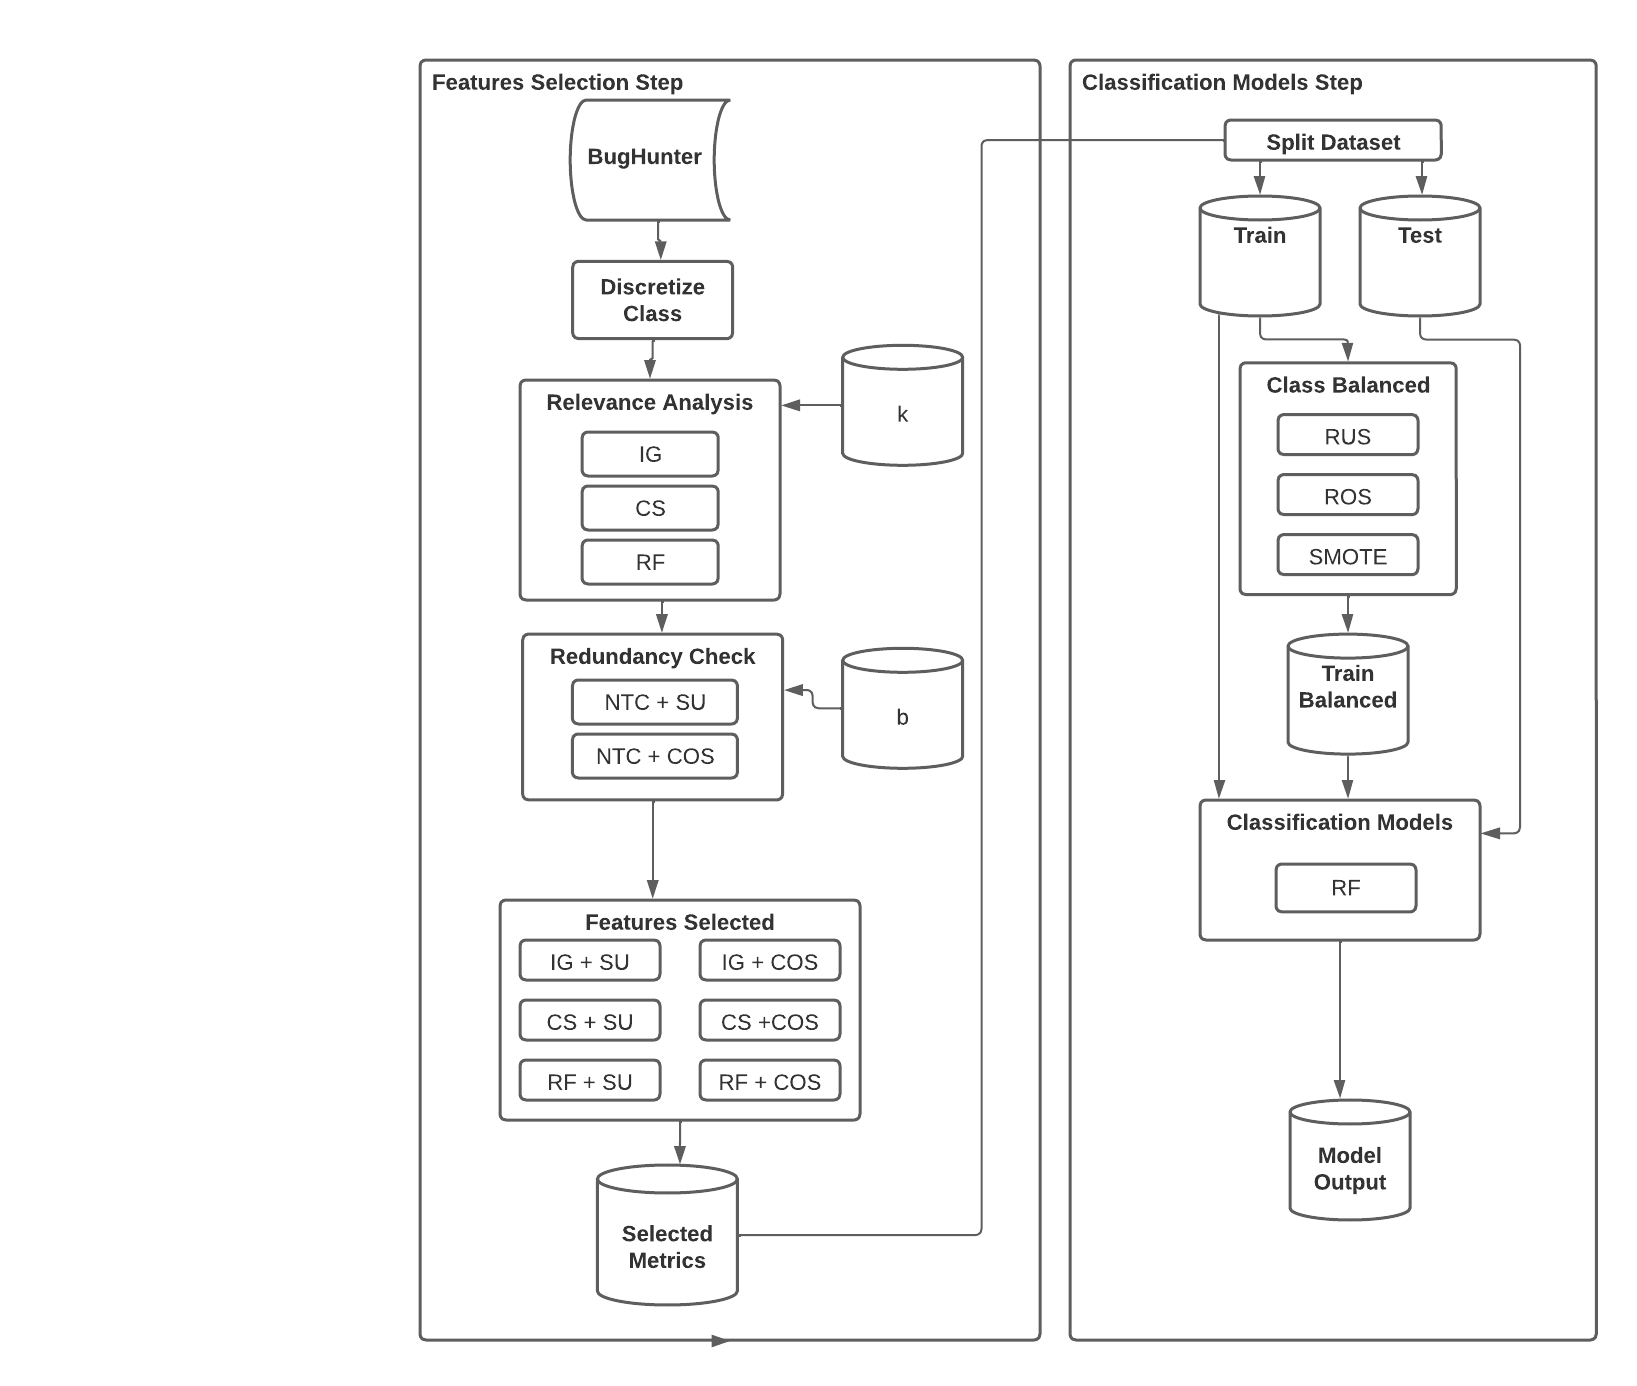
\includegraphics[width=150mm, height=110mm,]{figs/etapas/diagram.png}
    \captionsetup{labelsep=period, labelfont=bf}
    \setstretch{1} %Interlineado 1
    \caption{Descripción del flujo de trabajo}
    \label{fig:Flow}
\end{figure}

 El flujo descrito se ejecuta por cada proyecto iniciando con el proceso de selección de características. Cada proyecto contiene tres conjuntos de datos uno por cada nivel de métricas (Method, Class and File), el algoritmo \ref{alg:featureSelection} describe el primer paso del flujo \ref{fig:Flow}.
 
El algoritmo \ref{alg:featureSelection} describe el paso de Feature Selection. Se ejecuta ingresando cada conjunto de datos \(C_{p}(C_{\text{level}},C_{\text{class}},C_{\text{method}})\) donde \(_{p} \in \{p_{1},p_{2},...,p_{15}\}\) representa los 15 proyectos que contiene el BugHunter, y cada uno contiene tres conjuntos de datos, uno por cada nivel. Se guardan en la base de datos las métricas seleccionadas para cada nivel \(T_{\text{le}}(f_1,f_2,...,f_k)\) después de aplicar el análisis de relevancia y el control de redundancia. Utilizando tres ciclos anidados, se recorren las listas (\(rankList, bList, levelList\)) con la jerarquía \(rank \rightarrow \beta \rightarrow \text{level}\), donde \(rank\) se utiliza para seleccionar las métricas después del proceso de análisis de relevancia (IG, CS y RF), \(\beta\) es el umbral que se define para la ejecución del algoritmo NTC (análisis de redundancia), y \(\text{level}\) representa el nivel que se selecciona para el proyecto que se está analizando.

En cada iteración se lee el conjunto de datos (\(proyecto \rightarrow nivel\)) y se normaliza el atributo clase, dado que contiene valores numéricos que representan la cantidad de errores encontrados en esa medición, quedando solo con las clases BUG y NOBUG.

Se realiza el proceso de análisis de relevancia y el control de redundancia, y queda guardado en la base de datos qué métricas son seleccionadas en cada iteración y qué modelo de selección se utilizó, siendo este la combinación entre los algoritmos de relevancia y el control de redundancia. La lista queda como \(modelsSelections \rightarrow ['CS-SU','IG-SU','RF-SU','CS-COS','IG-COS','RF-COS']\).

 \begin{algorithm}[H]
    \hspace*{\algorithmicindent} \textbf{Input:} The original dataset $T_{le}(f_{1},f_{2},...,f_{k},l)$ where $l \in \{FP,NFP\}$ denotes the class label, and $k$ is the number of features. $le \in \{File, Class, Methods\}$ of a specific project

    \hspace*{\algorithmicindent} \textbf{Output:} Saves the selected characteristics in the Database. $T_{le}(f_1,f_2,...,f_k,l)$ where $k$ is the number of features selected by relevance analysis and redundancy check.
    \caption{Feature selection}
    \label{alg:featureSelection}
    \begin{algorithmic}[1]
    \fontsize{12pt}{12pt}\selectfont
    \REQUIRE $rankList \leftarrow [0.5, 0.7, 0.9]$
    \STATE $bList \leftarrow [0.5, 0.7, 0.9]$
    \STATE $levelList \leftarrow ['method', 'class', 'file']$
    \STATE $response \leftarrow \phi$

    \FOR{$\text{each}$ rank in $rankList$}
        \FOR{$\text{each}$ b in $bList$}
            \FOR{$\text{each}$ level in $levelList$}
                \STATE $data \leftarrow readDataset(level, project)$
                \STATE $data \leftarrow normalizeClass(data)$\;
                \STATE $square \leftarrow ChiSquare(data, rank)$\;
                \STATE $ig \leftarrow Ig(data, rank)$\;
                \STATE $relief \leftarrow ReliefF(data, rank)$\;
                \STATE $response \leftarrow response + NTC(b, square, 'CS-SU')$\;
                \STATE $response \leftarrow response + NTC(b, ig, 'IG-SU')$\;
                \STATE $response \leftarrow response + NTC(b, relief, 'RF-SU')$\;
                \STATE $response \leftarrow response + NTC(b, square, 'CS-COS')$\;
                \STATE $response \leftarrow response + NTC(b, ig, 'IG-COS')$\;
                \STATE $response \leftarrow response + NTC(b, relief, 'RF-COS')$\;
                \STATE $saveBD(response)$\;
            \ENDFOR
        \ENDFOR
    \ENDFOR
    \end{algorithmic}
\end{algorithm}

El algoritmo \ref{alg:executionmodels} representa el paso de modelos de clasificación. Se ingresan los mismos conjuntos de datos del algoritmo \ref{alg:featureSelection} pero $_{k}$ representa las métricas seleccionadas al ejecutar algoritmo \ref{alg:featureSelection}.

A los modelos de selección (\(modelsSelections\)) resultantes del algoritmo \ref{alg:executionmodels} se les agrega \(ALL\) que representa al conjunto de datos original sin realizar el paso de selección de características. Se agrega la lista de esquemas (\(modelsSelections\)) a los ciclos anidados. Quedando \(rank \rightarrow \beta \rightarrow level \rightarrow modelSelection\).

\begin{algorithm}[H]
    \hspace*{\algorithmicindent} \textbf{Input:} \\ The dataset $T_{le}(f_1, f_2, ..., f_k, l)$ where $l \in \{FP, NFP\}$ denotes the class label, and $k$ is the number of features selected by the feature selection process. $le \in \{File, Class, Methods\}$ of a specific project

    \hspace*{\algorithmicindent} \textbf{Output:} 
        Saves the precision, recall, accuracy, and f-measure in the Database 
    \caption{Execution of models}
    \label{alg:executionmodels}
    \begin{algorithmic}[1]
    \fontsize{12pt}{12pt}\selectfont
    \REQUIRE $rankList \leftarrow [0.5, 0.7, 0.9]$
    \STATE $rankList \leftarrow [0.5, 0.7, 0.9]$
    \STATE $bList \leftarrow [0.5, 0.7, 0.9]$
    \STATE $levelList \leftarrow ['method', 'class', 'file']$

    \STATE $modelsSelections \leftarrow ['CS-SU', 'IG-SU', 'RF-SU', 'CS-COS', 'IG-COS', 'RF-COS', 'ALL']$\;
    \STATE $response \leftarrow \phi$

    \FOR{$\text{each}$ rank in $rankList$}
        \FOR{$\text{each}$ b in $bList$}
            \FOR{$\text{each}$ level in $levelList$}
                \FOR{$\text{each}$ modelsSelection in $modelsSelections$}
                \STATE $data \leftarrow getData(rank, b, level, modelsSelection)$\;
                    \STATE $responseNormal \leftarrow ModelResult(data.original, model)$\;
                    \STATE $responseBalanced \leftarrow ModelResult(data.balanced, model)$\;
                    \STATE $saveBD(responseNormal)$\;
                    \STATE $saveBD(responseBalanced)$\;
                \ENDFOR
            \ENDFOR
        \ENDFOR
    \ENDFOR

    \end{algorithmic}
\end{algorithm}



En cada iteración se obtiene el conjunto de datos aplicando los filtros de métricas mencionados, este se utiliza para ejecutar los modelos de clasificación de la lista $models$. Los resultados de presision, recall y f-measure se almacenan en base de datos así como cada parámetro referente a la iteración para identificar a que conjunto de datos pertenecen y los parámetros de selección.





\section{La Medida de Rendimiento}

En el estudio principal se implementó el clasificador \textit{Random Forest} en la herramienta \textbf{Weka} \cite{weka}. Para la evaluación del modelo se utilizó la configuración \textit{Supplied Test Set}, que permite evaluar sobre un conjunto de prueba predefinido ---generado previamente en Python mediante partición estratificada 67/33---, de modo que todas las variantes de un mismo conjunto de datos se evalúan contra exactamente las mismas instancias.

El desempeño se mide con precisión, \textit{recall} y \textit{F-measure}, definidas en la Sección \ref{sec:metricas_evaluacion}. El valor de \textit{F-measure} reportado corresponde al agregado ponderado por la frecuencia de cada clase que entrega la herramienta para cada ejecución. De cada una de las ejecuciones del estudio principal se almacenaron esos valores agregados ---precisión, \textit{recall}, \textit{F-measure} y exactitud--- junto con los parámetros que identifican la configuración; no se conservaron las predicciones individuales ni las probabilidades estimadas. Las excepciones son la línea base del conjunto ``All'' a nivel de método, cuya salida completa de Weka se conservó (Tabla \ref{tab:porclase}), y las mejores configuraciones a nivel de método, de las que se conservó la matriz de confusión (Tabla \ref{table:weka_method_smote_b}). Por ello, las métricas por clase (\textit{F-measure} de la clase \textit{bug}, MCC y AUC-ROC) se obtienen de forma sistemática solo en el análisis de sensibilidad (Sección \ref{sec:sensibilidad}), diseñado para almacenarlas en todas sus ejecuciones.

El conjunto de datos tiene tres niveles de código fuente (método, clase y archivo) y 15 proyectos, además del conjunto resumido ``All''. La línea base se estableció con 2.592 ejecuciones y el estudio de selección de características y balanceo con 13.916 ejecuciones de \textit{Random Forest}; dado el tamaño de las tablas completas, se presentan los mejores resultados por proyecto y los agregados.

\section{Resultados con dataset original}
\label{sec:datasetoriginal}

En la sección actual, llevamos a cabo un experimento con el objetivo de replicar los resultados reportados en \cite{ferenc_automatically_2020}, enfocándonos en las métricas de código en distintos niveles. El estudio original aplicó once algoritmos de aprendizaje automático con cross validation de 10 folds en la herramienta WEKA sobre quince proyectos (y el dataset resumen), considerando tres niveles distintos en cada uno. En nuestro enfoque para replicar estos hallazgos, empleamos los mismos proyectos pero restringimos nuestra experimentación al algoritmo RandomForest de aprendizaje automático. Esta limitación se basó en la hipótesis de si sería posible alcanzar resultados comparables a los reportados en \cite{ferenc_automatically_2020}.

A continuación, presentamos en la Tabla \ref{table:original_result_average} una comparativa entre el promedio de nuestros resultados y los obtenidos en \cite{ferenc_automatically_2020}. Es importante señalar que, en nuestro experimento, se promediaron menos datos debido a la selección de una cantidad menor de algoritmos de aprendizaje automático para la prueba.

\begin{table}[H]
\captionsetup{labelsep=period, labelfont=bf}
\caption{\label{table:original_result_average} Resultado promedio de la medida f para nuestra investigación y el artículo que creó BugHunter }
\centering
\begin{tabular}{lll}
\toprule
       & Este trabajo       & Ferenc et al.     \\
\midrule
Nivel  & F-measure & F-measure \\
\hline
Método & 0,63      & 0,63      \\
Clase  & 0,50      & 0,56      \\
Archivo   & 0,50      & 0,54    \\
\bottomrule
\end{tabular}

\end{table}

Los resultados presentados en la Tabla \ref{table:original_result_average} revelan que, en promedio, nuestros hallazgos son comparables a pesar de haber realizado un número menor de experimentos. Esta observación nos permite afirmar, a nivel global, que hemos conseguido obtener resultados análogos a los reportados en \cite{ferenc_automatically_2020}. Tal similitud resalta la eficacia del algoritmo RandomForest en la evaluación de métricas de código en distintos niveles, y respalda la solidez del enfoque metodológico adoptado en el estudio original.

\subsection{Resultados Utilizando el Conjunto de Datos Original a Nivel de Método}
La Tabla \ref{table:original_result_weka_method_result} presenta los resultados de entrenar el modelo RandomForest con métricas a nivel de método para predecir fallos en este mismo nivel. La estructura de la tabla es la siguiente:

\begin{itemize}
  \item \textbf{Project:} Lista los proyectos de software analizados en el estudio. Cada uno representa una instancia de análisis individual y se incluye un conjunto denominado ALL, que es la unión de todos los proyectos.
  \item \textbf{F-measure:} Indica el valor de la medida F para cada proyecto, una métrica esencial en la valoración del rendimiento de modelos de aprendizaje automático, combinando precisión y recall.
\end{itemize}


\begin{table}[H]
\captionsetup{labelsep=period, labelfont=bf}
\caption{\label{table:original_result_weka_method_result} Resultados utilizando el conjunto de datos original a nivel de método}
\centering
{
\fontsize{12pt}{12pt}\selectfont
\begin{tabular}{ll}
\toprule
\multicolumn{2}{c}{MÉTODO} \\
\toprule
Proyecto                        & F-measure \\
\midrule
oryx                           & 0,852     \\
antlr4                         & 0,781     \\
BroadleafCommerce              & 0,778     \\
mct                            & 0,748     \\
junit                          & 0,695     \\
netty                          & 0,676     \\
ceylon-ide-eclipse             & 0,644     \\
titan                          & 0,584     \\
all                            & 0,579     \\
elasticsearch                  & 0,561     \\
mcMMO                          & 0,561     \\
orientdb                       & 0,56      \\
neo4j                          & 0,545     \\
hazelcast                      & 0,542     \\
MapDB                          & 0,52      \\
Android-Universal-Image-Loader & 0,486     \\
\bottomrule
\end{tabular}
}

\end{table}


El proyecto oryx obtuvo el mejor resultado a nivel de método con una F-measure de 0,85, mientras que en el estudio original de \cite{ferenc_automatically_2020}, el proyecto antlr4 mostró el mejor resultado con un valor de 0,75 \cite{ferenc_automatically_2020}. En nuestro análisis, el proyecto antlr4 alcanzó una F-measure de 0,78, lo que demuestra una similitud notable con los resultados originales. En el estudio de \cite{ferenc_automatically_2020}, el proyecto oryx tuvo una F-measure de 0,66, lo que indica la necesidad de un análisis más exhaustivo centrado en este proyecto para determinar las causas de la diferencia significativa de 0,19. Los demás proyectos mostraron valores comparables, con una variación promedio de ±0,10 en relación con los resultados del estudio original.

\begin{table}[H]
 \captionsetup{labelsep=period, labelfont=bf}
\caption{\label{table:original_result_weka_class_result} Resultados utilizando el conjunto de datos original a nivel de clase}
\centering
{
\fontsize{12pt}{10pt}\selectfont
\begin{tabular}{ll}
\toprule 
\multicolumn{2}{c}{CLASE} \\
\midrule 
Proyecto                        & F-measure \\
\hline 
oryx                           & 0,787     \\
BroadleafCommerce              & 0,687     \\
mct                            & 0,566     \\
junit                          & 0,543     \\
ceylon-ide-eclipse             & 0,533     \\
MapDB                          & 0,51      \\
all                            & 0,484     \\
hazelcast                      & 0,482     \\
elasticsearch                  & 0,481     \\
netty                          & 0,461     \\
orientdb                       & 0,456     \\
mcMMO                          & 0,446     \\
titan                          & 0,397     \\
antlr4                         & 0,387     \\
Android-Universal-Image-Loader & 0,358     \\
neo4j                          & 0,338    \\
\bottomrule
\end{tabular}
}

\end{table}


En lo que respecta a las métricas de código a nivel de clases, observamos una variación promedio de ±0,10 en todos los proyectos. Esta discrepancia podría atribuirse al uso de una mayor variedad de algoritmos de aprendizaje automático en el estudio original. No obstante, hemos conseguido resultados comparables, logrando así cumplir con nuestro objetivo inicial. Es importante resaltar que, una vez más, el proyecto oryx se posiciona a la cabeza en este nivel, mostrando una mínima diferencia de 0,08 en la F-measure en comparación con el estudio original. Este hallazgo es notable considerando que, en el análisis original a nivel de clase, el mejor desempeño lo obtuvo BroadleafCommerce con una F-measure de 0,74 utilizando el algoritmo RandomForest. Estos resultados subrayan la consistencia de oryx en nuestros experimentos y reflejan la efectividad del algoritmo RandomForest en diferentes contextos y niveles de métrica.

\begin{table}[H]
\captionsetup{labelsep=period, labelfont=bf}
\caption{\label{table:original_result_weka_file_result} Resultados utilizando el conjunto de datos original a nivel de archivo}
\centering
{
\fontsize{12pt}{10pt}\selectfont
\begin{tabular}{ll}
\toprule 
\multicolumn{2}{c}{ARCHIVO} \\
\midrule 
Proyecto                        & F-measure \\
\hline 
oryx                           & 0,77      \\
BroadleafCommerce              & 0,67      \\
mct                            & 0,586     \\
ceylon-ide-eclipse             & 0,541     \\
antlr4                         & 0,501     \\
all                            & 0,482     \\
elasticsearch                  & 0,474     \\
hazelcast                      & 0,474     \\
orientdb                       & 0,47      \\
junit                          & 0,468     \\
netty                          & 0,45      \\
mcMMO                          & 0,447     \\
MapDB                          & 0,444     \\
titan                          & 0,436     \\
neo4j                          & 0,362     \\
Android-Universal-Image-Loader & 0,344    \\
\bottomrule
\end{tabular}
}

\end{table}


Al considerar las métricas a nivel de archivo, nuevamente destacamos que el proyecto oryx obtuvo el mejor resultado con una F-measure de 0,77. Esto contrasta con los hallazgos del estudio original, donde el proyecto BroadleafCommerce lideró con una F-measure de 0,77, seguido por oryx con 0,64, lo cual representa una diferencia de 0,13 en comparación con nuestros resultados. En este nivel, también observamos una variación promedio de ±0,10 en los valores obtenidos para la F-measure.

Estos experimentos han permitido alinear nuestros resultados iniciales con aquellos reportados en el estudio original, estableciendo una base sólida para futuras mejoras. Estas mejoras se centrarán en la reducción del número de métricas utilizadas en los algoritmos de aprendizaje automático, manteniendo o incluso superando los resultados obtenidos en esta fase experimental. Para todos los proyectos, a nivel de método se introducen 72 características en los algoritmos, a nivel de clase 92, y a nivel de archivo 6. Por tanto, el objetivo será minimizar el número de características introducidas, buscando optimizar la eficacia y eficiencia de los modelos de predicción empleados.

\subsection{Desglose por clase de la línea base}

La salida completa de Weka para la línea base del conjunto ``All'' a nivel de método se conservó, lo que permite desglosar su desempeño por clase (Tabla \ref{tab:porclase}). El contraste es ilustrativo: el \textit{F-measure} ponderado de 0,565 encubre un \textit{F-measure} de solo 0,356 para la clase \textit{bug} (precisión de 0,410 y \textit{recall} de 0,314), con un MCC de 0,052 y un AUC-ROC de 0,539, valores apenas superiores a los de un clasificador aleatorio. Este desglose cuantifica de forma directa cuánto puede encubrir la métrica agregada respecto de la clase de interés práctico (Sección \ref{sec:RQ4}), y es coherente con el desempeño no superior del conjunto unificado frente a los proyectos individuales (RQ5).

\begin{table}[H]
\centering
\caption{Desglose por clase de la línea base (Weka, Random Forest, validación cruzada de 10 particiones) sobre el conjunto ``All'' a nivel de método}
\label{tab:porclase}
\begin{tabular}{lccccc}
\toprule
Clase & Precisión & \textit{Recall} & \textit{F-measure} & MCC & AUC-ROC \\
\midrule
No-bug & 0,646 & 0,735 & 0,688 & 0,052 & 0,539 \\
Bug    & 0,410 & 0,314 & 0,356 & ---   & ---   \\
\midrule
Prom. ponderado & 0,559 & 0,579 & 0,565 & 0,052 & 0,539 \\
\bottomrule
\end{tabular}
\end{table}


\section{Experimento exploratorio preliminar en Python}
\label{sec:exploratorio_python}

Antes del estudio principal se realizó un experimento exploratorio en Python, a nivel de método, con tres clasificadores (\textit{Random Forest}, árbol de decisión y Naive Bayes). Su objetivo fue examinar el efecto de aplicar el balanceo de clases antes o después de la partición en entrenamiento y prueba. Sus resultados no responden directamente a las preguntas de investigación ---que se responden con el estudio principal en Weka (Secciones \ref{sec:RQ1} a \ref{sec:RQ5})---, sino que motivaron la decisión metodológica de balancear exclusivamente el conjunto de entrenamiento. Según el código conservado, en la variante que balancea solo el entrenamiento las métricas se calcularon para la clase positiva (\textit{bug}); el tipo de promedio de la variante que balancea el conjunto completo no pudo verificarse. Se emplearon las siguientes bibliotecas:

\begin{itemize}
    \item \textbf{Pandas:} Utilizada para la manipulación y análisis de datos, facilitando la carga, procesamiento y visualización de los conjuntos de datos.
    \item \textbf{NumPy:} Empleada para operaciones matemáticas y manipulación de arreglos, complementando a Pandas en el manejo eficiente de datos numéricos.
    \item \textbf{Scikit-learn:} Biblioteca utilizada para el preprocesamiento de datos, la partición en entrenamiento y prueba y la implementación de los modelos de clasificación de este experimento.
    \item \textbf{Imbalanced-learn:} Utilizada específicamente para técnicas de balanceo de clases, incluyendo ROS (Random Over Sampling), RUS (Random Under Sampling) y SMOTE (Synthetic Minority Over-sampling Technique).
    \item \textbf{Matplotlib y Seaborn:} Empleadas para la visualización de datos y resultados, generando gráficos y figuras que facilitan la interpretación de los resultados obtenidos.
\end{itemize}

En una primera variante del experimento, las técnicas de balanceo se aplicaron al conjunto de datos completo, antes de la partición. Esto implica que tanto el conjunto de entrenamiento como el de prueba pueden contener instancias generadas artificialmente o duplicadas, según el algoritmo de balanceo utilizado; en una segunda variante, el balanceo se aplicó solo al entrenamiento.


\subsection{Consecuencias negativas de balancear el conjunto completo}

En los modelos de clasificación utilizados en los experimentos, aplicar técnicas de balanceo a todo el conjunto de datos, incluyendo tanto el conjunto de entrenamiento como el de prueba, puede acarrear varias consecuencias negativas:

\begin{itemize}
    \item \textbf{Sobreajuste (Overfitting):} La inclusión de datos artificialmente generados en el conjunto de entrenamiento puede causar que el modelo se ajuste demasiado a estos datos sintéticos, disminuyendo su capacidad para generalizar correctamente a datos nuevos y no vistos.
    \item \textbf{Evaluación Sesgada:} Si el conjunto de prueba también contiene datos balanceados artificialmente, las métricas de evaluación pueden no reflejar el rendimiento real del modelo en un entorno no balanceado. Esto podría llevar a una sobreestimación de la capacidad predictiva del modelo.
    \item \textbf{Redundancia de Datos:} Los métodos de sobrerrepresentación (ROS y SMOTE) pueden introducir múltiples copias o variaciones de los mismos datos, lo que puede redundar en una menor diversidad dentro del conjunto de datos y afectar negativamente la capacidad del modelo para aprender patrones generalizables.
    \item \textbf{Pérdida de Información:} Los métodos de subrepresentación (RUS) eliminan datos de las clases mayoritarias, lo que puede llevar a la pérdida de información valiosa y afectar la capacidad del modelo para capturar la complejidad inherente de los datos originales.
    \item \textbf{Introducción de Ruido:} Los datos sintéticos generados por SMOTE pueden introducir ruido en el conjunto de datos si las nuevas instancias no reflejan adecuadamente las características del problema real, lo que puede afectar negativamente el rendimiento del modelo.
\end{itemize}

Para mitigar estas consecuencias, es recomendable aplicar las técnicas de balanceo únicamente al conjunto de entrenamiento, manteniendo el conjunto de prueba en su estado original. Esto asegura que la evaluación del modelo refleje con mayor precisión su desempeño en condiciones reales y no sesgadas.

Las tablas presentadas a continuación resumen los resultados de ambas variantes a nivel de método.

\subsection{Resultados balanceando todo el conjunto de datos}

Los valores de esta subsección están inflados por la fuga de información descrita: el conjunto de prueba contiene instancias duplicadas o sintéticas derivadas de las del entrenamiento, por lo que no reflejan el desempeño en condiciones reales. La Tabla \ref{tab:ros_results} presenta los resultados obtenidos al aplicar la técnica de Sobremuestreo Aleatorio (ROS) al conjunto completo. El algoritmo Random Forest (RF) alcanzó una F-measure de 0.95, con una precisión de 0.9 y un recall perfecto de 1, lo que indica un rendimiento excelente bajo esta técnica. Decision Tree (DT) obtuvo un valor de F-measure idéntico, con los mismos valores de precisión y recall que RF. Por otro lado, Naive Bayes (NB) presentó una F-measure de 0.69, con una precisión de 0.56 y un recall de 0.89, siendo inferior a RF y DT pero aún así notable en términos de recall.


\begin{table}[H]
\centering
\captionsetup{labelsep=period, labelfont=bf}
\caption{Resultados de los algoritmos utilizando ROS}
\fontsize{12pt}{10pt}\selectfont
\begin{tabular}{llll}
\toprule 
\textbf{Algorithm} & \textbf{Precision} & \textbf{Recall} & \textbf{F-measure} \\ 
\midrule 
RF & 0.9 & 1 & 0.95 \\ 
DT & 0.9 & 1 & 0.95 \\ 
NB & 0.56 & 0.89 & 0.69 \\ 
\bottomrule
\end{tabular}

\label{tab:ros_results}
\end{table}



En la Tabla \ref{tab:rus_results} se muestran los resultados de los algoritmos de clasificación utilizando la técnica de Submuestreo Aleatorio (RUS). DT alcanzó una F-measure de 0.85, con una precisión de 0.93 y un recall de 0.82, mostrando un equilibrio sólido entre precisión y recall. RF obtuvo una F-measure de 0.77, con una precisión de 0.82 y un recall de 0.78, mientras que NB logró una F-measure de 0.68, con una precisión de 0.55 y un recall de 0.89, destacándose más en el recall.


\begin{table}[H]
\centering
\captionsetup{labelsep=period, labelfont=bf}
\caption{Resultados de los algoritmos utilizando RUS}
\fontsize{12pt}{10pt}\selectfont
\begin{tabular}{llll}
\toprule 
\textbf{Algorithm} & \textbf{Precision} & \textbf{Recall} & \textbf{F-measure} \\ 
\midrule 
DT & 0.93 & 0.82 & 0.85 \\ 
RF & 0.82 & 0.78 & 0.77 \\ 
NB & 0.55 & 0.89 & 0.68 \\ 
\bottomrule
\end{tabular}

\label{tab:rus_results}
\end{table}


La Tabla \ref{tab:smote_results} resume los resultados al aplicar la técnica SMOTE. El algoritmo RF obtuvo una F-measure de 0.88, con una precisión de 0.89 y un recall de 0.89, destacándose nuevamente como el mejor desempeño. DT logró una F-measure de 0.85, con una precisión de 0.87 y un recall de 0.83, siendo ligeramente inferior a RF. NB presentó una F-measure de 0.70, con una precisión de 0.56 y un recall de 0.92, mostrando una vez más un alto recall.


\begin{table}[H]
\centering
\captionsetup{labelsep=period, labelfont=bf}
\caption{Resultados de los algoritmos utilizando SMOTE}
\fontsize{12pt}{10pt}\selectfont
\begin{tabular}{llll}
\toprule 
\textbf{Algorithm} & \textbf{Precision} & \textbf{Recall} & \textbf{F-measure} \\ 
\midrule 
RF & 0.89 & 0.89 & 0.88 \\ 
DT & 0.87 & 0.83 & 0.85 \\ 
NB & 0.56 & 0.92 & 0.70 \\ 
\bottomrule
\end{tabular}

\label{tab:smote_results}
\end{table}


Los resultados sin aplicar ninguna técnica de balanceo se presentan en la Tabla \ref{tab:none_results}. NB mostró una F-measure de 0.47, con una precisión de 0.37 y un recall de 0.76, mientras que RF obtuvo una F-measure de 0.40, con una precisión de 0.49 y un recall de 0.35. DT alcanzó una F-measure de 0.42, con una precisión de 0.43 y un recall de 0.41. Estos resultados reflejan el impacto negativo del desequilibrio de clases en el rendimiento de los algoritmos, con un notable descenso en la precisión.

\begin{table}[H]
\centering
\captionsetup{labelsep=period, labelfont=bf}
\caption{Resultados de los algoritmos sin técnicas de balanceo}
\fontsize{12pt}{10pt}\selectfont
\begin{tabular}{llll}
\toprule 
\textbf{Algorithm} & \textbf{Precision} & \textbf{Recall} & \textbf{F-measure} \\ 
\midrule 
NB & 0.37 & 0.76 & 0.47 \\ 
DT & 0.43 & 0.41 & 0.42 \\ 
RF & 0.49 & 0.35 & 0.40 \\ 
\bottomrule
\end{tabular}

\label{tab:none_results}
\end{table}


Finalmente, la Tabla \ref{tab:best_f_measure} proporciona una visión general de los mejores valores de F-measure obtenidos por diferentes proyectos a nivel de método. El proyecto ``oryx'' alcanzó la F-measure más alta de 0.88 utilizando RF, seguido de ``antlr4'' con una F-measure de 0.87 también con RF. En términos de precisión y recall, ``oryx'' mostró una precisión de 0.89 y un recall de 0.89, mientras que ``antlr4'' tuvo una precisión de 0.87 y un recall de 0.83. En contraste, los proyectos ``mct'' y ``BroadleafCommerce'' lograron F-measures de 0.82 y 0.78 respectivamente, utilizando RF, con valores de precisión y recall consistentes. ``junit'' y ``netty'' obtuvieron F-measures de 0.77 y 0.72 respectivamente, también utilizando RF, manteniendo un equilibrio adecuado entre precisión y recall.

\begin{table}[H]
\centering
\captionsetup{labelsep=period, labelfont=bf}
\caption{Los mejores valores de F-measure por proyecto a nivel de método}
\fontsize{12pt}{10pt}\selectfont
\begin{tabular}{lll}
\toprule 
\textbf{Project} & \textbf{F-measure} & \textbf{Algorithm} \\ \midrule 
oryx & 0.88 & RF \\ 
antlr4 & 0.87 & RF \\ 
mct & 0.82 & RF \\ 
BroadleafCommerce & 0.78 & RF \\ 
junit & 0.77 & RF \\ 
netty & 0.72 & RF \\ 
titan & 0.72 & RF \\ 
ceylon-ide-eclipse & 0.71 & RF \\ 
mcMMO & 0.66 & NB \\ 
elasticsearch & 0.62 & NB \\ 
\bottomrule
\end{tabular}

\label{tab:best_f_measure}
\end{table}


\subsection{Resultados balanceando solo conjunto de datos de entrenamiento}

Buscando mitigar las consecuencias negativas descritas anteriormente, se realizan nuevos experimentos balanceando solo el conjunto de datos de entrenamiento evitando la posibilidad de que existan datos generados o duplicados en el conjunto de pruebas.

\subsubsection{Resultados Utilizando ROS}
La Tabla \ref{tab:results_ros_sin} presenta los resultados de aplicar el algoritmo ROS (Random Over Sampling) únicamente al conjunto de datos de entrenamiento. Este método incrementa artificialmente el número de instancias de la clase minoritaria mediante duplicación. Los resultados muestran que el modelo Naive Bayes (NB) alcanzó una precisión de 0.37, un recall de 0.97 y una F-measure de 0.54. Este alto valor de recall indica que el modelo es efectivo en identificar la mayoría de las instancias de la clase minoritaria, aunque a costa de una baja precisión, lo que sugiere muchos falsos positivos. El Random Forest (RF) y el Decision Tree (DT) mostraron un desempeño más equilibrado en términos de precisión y recall, aunque con valores más bajos comparados con NB. RF alcanzó una precisión de 0.53, un recall de 0.48 y una F-measure de 0.50, mientras que DT mostró una precisión de 0.38, un recall de 0.60 y una F-measure de 0.46.


\begin{table}[H]
\centering
\caption{Resultado de los algoritmos utilizando ROS con balanceo solo al conjunto de entrenamiento}
\captionsetup{labelsep=period, labelfont=bf}
\fontsize{12pt}{10pt}\selectfont
\begin{tabular}{lccc}
\toprule 
\textbf{Modelo} & \textbf{Precisión} & \textbf{Recall} & \textbf{F-measure} \\
\midrule  
NB & 0.37 & 0.97 & 0.54 \\
RF & 0.53 & 0.48 & 0.50 \\
DT & 0.38 & 0.60 & 0.46 \\
\bottomrule
\end{tabular}
\label{tab:results_ros_sin}
\end{table}


\subsubsection{Resultados Utilizando RUS}
La Tabla \ref{tab:results_rus_sin} muestra los resultados de aplicar el algoritmo RUS (Random Under Sampling) solo al conjunto de entrenamiento. Este método reduce el número de instancias de la clase mayoritaria para equilibrar el dataset. Los resultados indican que NB mantiene su rendimiento con una precisión de 0.37, un recall de 0.97 y una F-measure de 0.54. Sin embargo, se observan mejoras en RF y DT comparados con los resultados obtenidos con ROS. RF mejora su precisión a 0.43 y su recall a 0.59, obteniendo una F-measure de 0.50, mientras que DT mejora en precisión a 0.43 y en recall a 0.58, logrando una F-measure de 0.49. Esto sugiere que RUS puede ser más efectivo que ROS para estos algoritmos al mejorar la representación de la clase minoritaria sin introducir demasiados falsos positivos.


\begin{table}[H]
\centering
\captionsetup{labelsep=period, labelfont=bf}
\caption{Resultado de los algoritmos utilizando RUS con balanceo solo al conjunto de entrenamiento}
\fontsize{12pt}{10pt}\selectfont
\begin{tabular}{lccc}
\toprule 
\textbf{Algorithm} & \textbf{Precisión} & \textbf{Recall} & \textbf{F-measure} \\
\midrule 
NB & 0.37 & 0.97 & 0.54 \\
RF & 0.43 & 0.59 & 0.50 \\
DT & 0.43 & 0.58 & 0.49 \\
\bottomrule
\end{tabular}
\label{tab:results_rus_sin}
\end{table}




\subsubsection{Resultados Utilizando SMOTE}

La Tabla \ref{tab:results_smote_sin} detalla los resultados de utilizar SMOTE (Synthetic Minority Over-sampling Technique) para balancear el conjunto de entrenamiento. SMOTE genera nuevas instancias sintéticas de la clase minoritaria mediante interpolación. En este caso, DT muestra una notable mejora con una precisión de 0.50, un recall de 0.80 y una F-measure de 0.62. RF también mejora, alcanzando una precisión de 0.44, un recall de 0.80 y una F-measure de 0.57. NB, sin embargo, mantiene sus valores constantes con una precisión de 0.37, un recall de 0.97 y una F-measure de 0.54. Comparados con la Tabla \ref{tab:none_results} (sin balanceo), estos resultados muestran que balancear solo el entrenamiento eleva sobre todo el \textit{recall} de la clase \textit{bug}, a costa de la precisión. Es el mismo intercambio que el estudio principal y el análisis de sensibilidad cuantifican de forma sistemática (Secciones \ref{sec:RQ4} y \ref{sec:sensibilidad}).

La comparación entre ambas variantes ---valores de \textit{F-measure} de hasta 0,95 balanceando el conjunto completo frente a valores de entre 0,46 y 0,62 balanceando solo el entrenamiento--- ilustra la magnitud del sesgo que introduce balancear antes de la partición, y justifica que en el resto de la tesis el balanceo se aplique exclusivamente sobre el conjunto de entrenamiento.


\begin{table}[H]
\centering
\captionsetup{labelsep=period, labelfont=bf}
\caption{Resultado de los algoritmos utilizando SMOTE con balanceo solo al conjunto de entrenamiento}
\fontsize{12pt}{10pt}\selectfont
\begin{tabular}{lccc}
\hline
\textbf{Modelo} & \textbf{Precisión} & \textbf{Recall} & \textbf{F-measure} \\
\hline
DT & 0.50 & 0.80 & 0.62 \\
RF & 0.44 & 0.80 & 0.57 \\
NB & 0.37 & 0.97 & 0.54 \\
\hline
\end{tabular}

\label{tab:results_smote_sin}
\end{table}




En esta sección se estudian las cinco preguntas de investigación a partir de los resultados experimentales. La discusión de los hallazgos y las amenazas a la validez se presentan en el Capítulo \ref{cap:discusion}.

\section{Primera pregunta de investigación}
La primera pregunta de investigación a responder es:
\label{sec:RQ1}

\noindent\fbox{%
\parbox{\dimexpr\textwidth-2\fboxsep-2\fboxrule\relax}{%
\textbf{RQ1} ¿El análisis de relevancia y control de redundancia de características puede mejorar la identificación de bugs basado en métricas de código?%
}%
}
\vspace{12pt}

Para abordar la pregunta de investigación \textbf{RQ1} se condujo un experimento de 13.916 ejecuciones del clasificador \textit{Random Forest}. Cada conjunto proyecto-nivel se recorrió (Figura \ref{fig:Flow}) a través del espacio de parámetros definido por el umbral de relevancia (\textit{Rank}), el umbral de redundancia $\beta$ y el esquema de selección. En cada iteración se generaron en Python un conjunto de prueba con el 33\,\% de los datos, mediante partición estratificada, y dos conjuntos de entrenamiento: uno con la distribución de clases original y otro balanceado con ROS, RUS o SMOTE, técnicas aplicadas exclusivamente sobre el entrenamiento. Ambos conjuntos de entrenamiento se utilizaron para entrenar \textit{Random Forest} en la plataforma \textit{Weka}, en la modalidad \textit{Supplied test set}, evaluando siempre contra el mismo conjunto de prueba, lo que permite una comparación directa de su rendimiento. La consistencia de este flujo con una implementación equivalente en \textit{scikit-learn} se verifica en la Sección \ref{sec:validacion_flujos}.

Comparamos los resultados obtenidos con la selección de características con los resultados base obtenidos sin selección de características en la sección anterior. 

\subsection{Método}
 A nivel de método, los mejores resultados se obtienen con el proyecto Oryx, que alcanza una medida F de 0,838 y 0,837, sin balancear y balanceando las clases, respectivamente. Estos resultados se logran con 29 y 4 características, respectivamente, lo que supone una reducción del 59,7 \% y del 94,4 \% respecto a las 72 características que se usan en los resultados base. Los resultados base muestran que el proyecto Oryx tiene una medida F de 0,852, por lo que la diferencia con la selección de características es de solo 0,014. Esto indica que la selección de características permite mantener un rendimiento similar al de los resultados base, pero con una reducción significativa de la dimensionalidad de los datos. Además, esto sugiere que muchas de las características originales podrían ser irrelevantes o redundantes para la predicción de defectos de software. 

La tabla \ref{table:b_u_c_m} resume los resultados a nivel de método. 
\input{chapters/chapter3/Sections/Research Questions/sections/RQ1/tables/method}

\subsection{Clase}
A nivel de clase, el proyecto Oryx también obtiene los mejores resultados, con una medida F de 0,78 tanto sin balancear como balanceando las clases. Sin embargo, la selección de características permite reducir el número de características de 92 a 6 y 47, respectivamente. Esto implica una reducción del 93,5 \% y del 48,9 \% respecto a los resultados base, que usan todas las características. Por lo tanto, la selección de características también es beneficiosa a nivel de clase, ya que permite simplificar el modelo sin perder rendimiento.
La tabla \ref{table:b_u_c_c} resume los resultados a nivel de clase.

\input{chapters/chapter3/Sections/Research Questions/sections/RQ1/tables/class}
\subsection{Archivo}
A nivel de archivo, el proyecto Oryx vuelve a obtener los mejores resultados, con una medida F de 0,806 con la selección de características y sin balancear las clases (0,777 balanceando). Este resultado mejora en 0,036 el resultado base, que tiene una medida F de 0,770 con todas las características. Además, la selección de características permite reducir el número de características de 6 a 3, lo que supone una reducción del 50\,\%. Así, la selección de características mejora el rendimiento y la simplicidad del modelo a nivel de archivo.

La tabla \ref{table:b_u_c_f} resume los resultados a nivel de archivo.
\input{chapters/chapter3/Sections/Research Questions/sections/RQ1/tables/file}

\subsection{Resultados agregados sobre los 15 proyectos}

El patrón observado en Oryx se confirma al agregar los 15 proyectos individuales (Tabla \ref{tab:agg}): la mediana del mejor \textit{F-measure} apenas varía entre las versiones sin balancear y balanceada en los tres niveles, con reducciones medianas del número de características del 40\,\% a nivel de método, 88\,\% a nivel de clase y 50\,\% a nivel de archivo. En cuanto a los esquemas, la Semejanza de Coseno (COS) predominó en el control de redundancia a nivel de método y archivo, mientras que la Incertidumbre Simétrica (SU) fue más frecuente a nivel de clase.

\begin{table}[H]
\centering
\caption{Mejor \textit{F-measure} por proyecto agregado sobre los 15 proyectos individuales (mediana [mín--máx])}
\label{tab:agg}
\begin{tabular}{lcc}
\toprule
Nivel & Sin balancear & Balanceado \\
\midrule
Método  & 0,620 [0,538--0,838] & 0,615 [0,525--0,837] \\
Clase   & 0,524 [0,448--0,786] & 0,519 [0,460--0,780] \\
Archivo & 0,525 [0,456--0,806] & 0,547 [0,436--0,777] \\
\bottomrule
\end{tabular}
\end{table}

\textit{Advertencia sobre el sesgo de comparar el mejor esquema contra una única configuración de referencia.} Las Tablas \ref{table:b_u_c_m}, \ref{table:b_u_c_c}, \ref{table:b_u_c_f} y \ref{tab:agg} comparan el mejor esquema de selección ---un máximo sobre las 54 combinaciones de algoritmo de relevancia, medida de redundancia, \textit{Rank} y $\beta$--- frente a una única configuración de referencia (todas las características). Esta comparación introduce una asimetría optimista estructural que, a diferencia de lo que ocurre en RQ4, no se cancela con una comparación simétrica. Por ello, la evidencia más robusta de RQ1 corresponde a las medianas de la Tabla \ref{tab:agg} y a las del análisis de sensibilidad (Sección \ref{sec:sensibilidad}), antes que a la cifra máxima de 94\,\% obtenida en una única celda (proyecto Oryx, nivel método). La eliminación completa de este sesgo, seleccionando el esquema sobre una partición de validación independiente de la de prueba, se declara como trabajo futuro (Capítulo \ref{cap:conclusion}).


\noindent\fbox{%
\parbox{\dimexpr\textwidth-2\fboxsep-2\fboxrule\relax}{%
\textbf{Respuesta RQ1} Los hallazgos experimentales corroboran la eficacia de las estrategias implementadas para el análisis de relevancia y la mitigación de redundancia, las cuales han facilitado una compresiva reducción de características manteniendo la integridad de los resultados iniciales. Específicamente, el algoritmo de \textit{Semejanza de Coseno} (COS) se identificó como preponderante para el nivel de método y archivo, mientras que la \textit{Incertidumbre Simétrica} (SU) fue preeminente a nivel de clases. Estas técnicas reducen la mediana del número de métricas en un 40\,\%, 88\,\% y 50\,\% en los niveles de método, clase y archivo, respectivamente (hasta un 94\,\% en el mejor caso individual), con una pérdida de \textit{F-measure} inferior a 0,02. El análisis de sensibilidad (Sección \ref{sec:sensibilidad}) confirma que este resultado se mantiene con XGBoost y SVM lineal.

}%
}
\vspace{12pt}





\section{Segunda pregunta de investigación}
\label{sec:RQ2}

\noindent\fbox{%
\parbox{\dimexpr\textwidth-2\fboxsep-2\fboxrule\relax}{%
\textbf{RQ2} ¿Cuales métricas de código fuente son buenas predictoras de errores y en que tipo de métrica (archivo, clase,
método) proporciona mejores resultados?%
}%
}
\vspace{12pt}

Se implementaron 6 algoritmos de selección de características (\ref{fig:Flow}) y al terminar cada etapa, se registran todos los resultados pertinentes, incluyendo las métricas seleccionadas por cada algoritmo y los distintos valores de rank y $\beta$ utilizados.

Posteriormente, se realizó un análisis de la frecuencia de aparición de cada métrica en todos los algoritmos de selección. Ordenando los resultados desencendentemente por la suma de la frecuencia de aparición de cada métrica en los seis esquemas de selección utilizados. Como resultado, se identificaron las 23 métricas con mayor frecuencia de aparición, cuyos detalles se ilustran en \ref{fig:sum_frecuency}.

\begin{figure}[H]
	\centering
	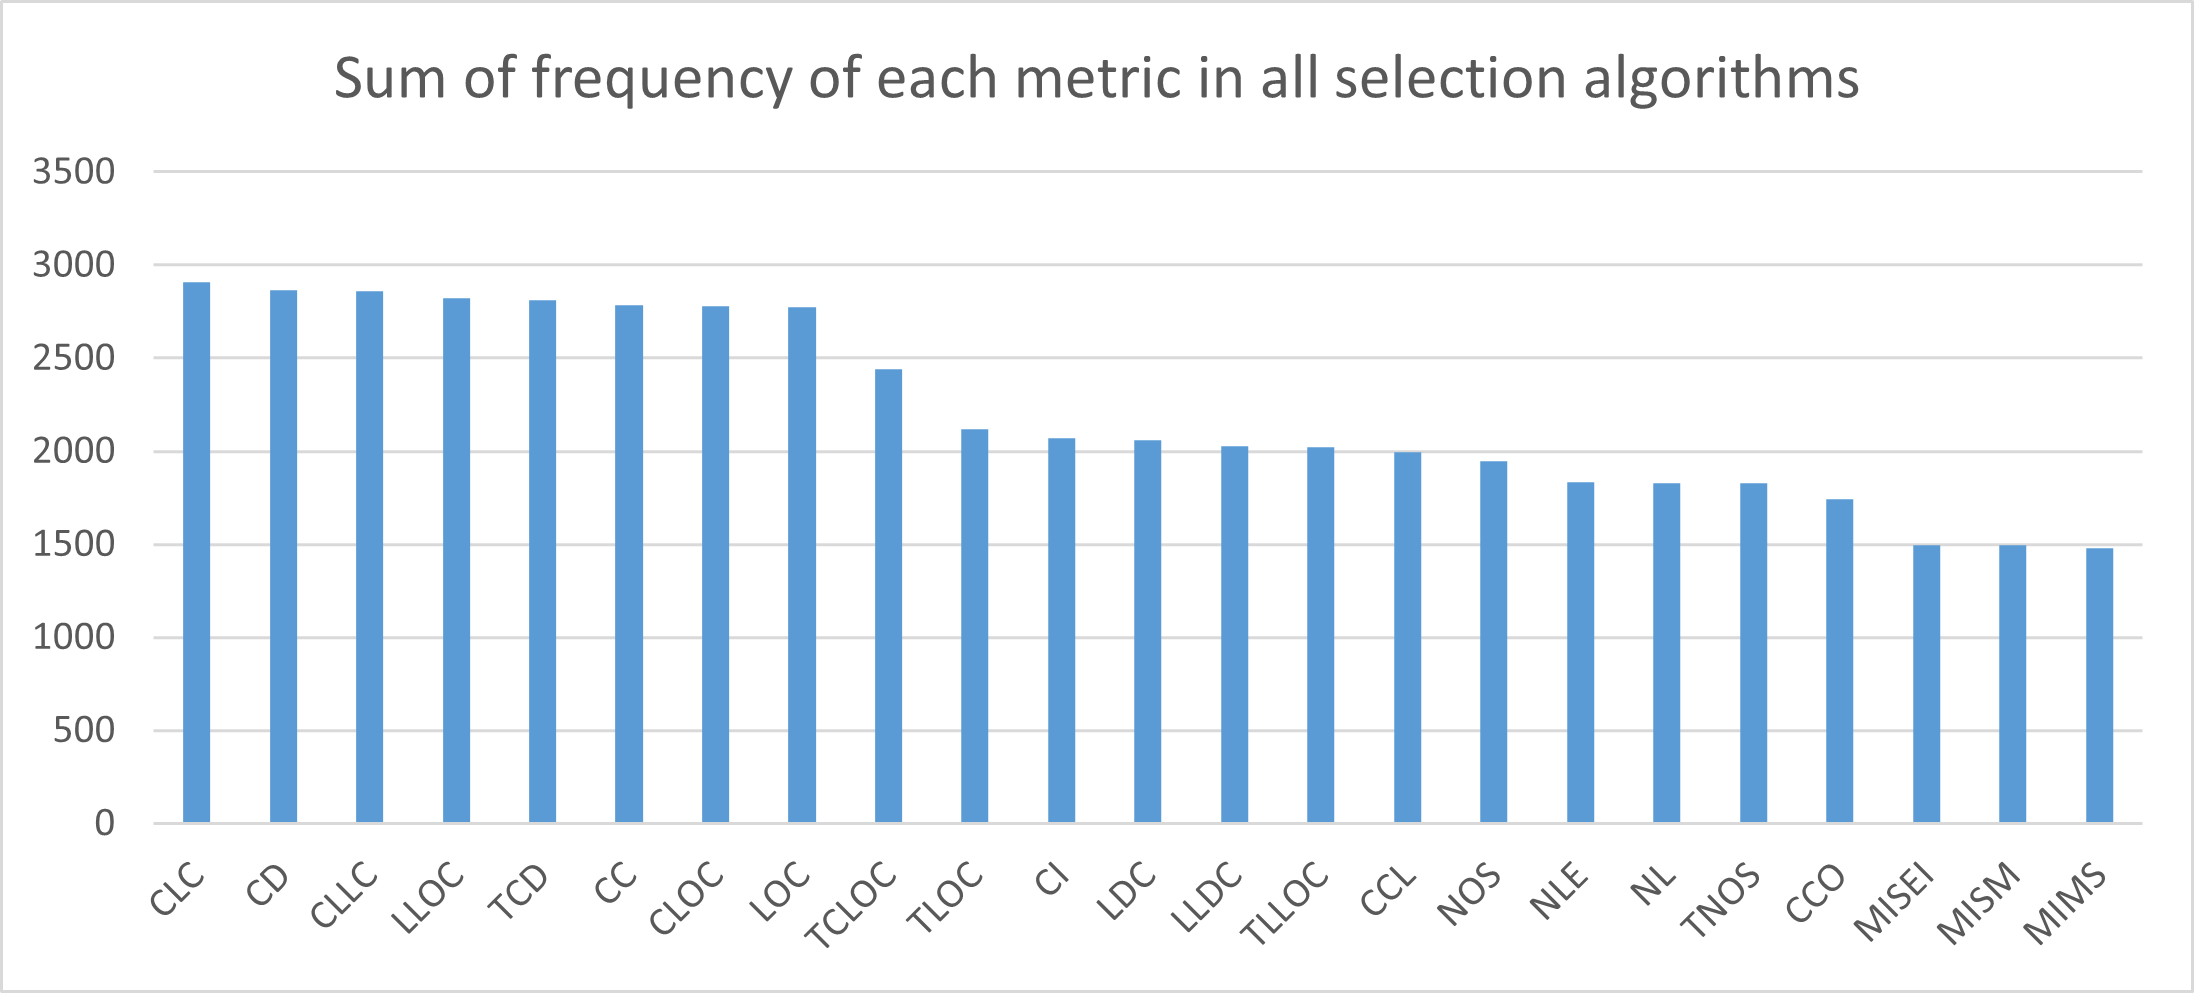
\includegraphics[scale=0.9]{chapters/chapter3/Sections/Research Questions/sections/RQ2/img/frec_all.png} %Change the figure name 
	\setstretch{1} %Interlineado 1
	\captionsetup{labelsep=period, labelfont=bf}
	\caption[Suma de la frecuencia de aparición de cada métrica en todos los algoritmos de selección]{Suma de la frecuencia de aparición de cada métrica en todos los algoritmos de selección} %[Se muestra en el índice]{Se muestra en el pie de figura}
	\label{fig:sum_frecuency}
\end{figure}


En la figura \ref{fig:frecuencyby}, se observa un patrón consistente: en promedio, los algoritmos de selección que incorporan el algoritmo de SU en su etapa de control de redundancia tienden a resultar en un menor número de características seleccionadas, en comparación con aquellos que utilizan la COS.

\begin{figure}[H]
	\centering
	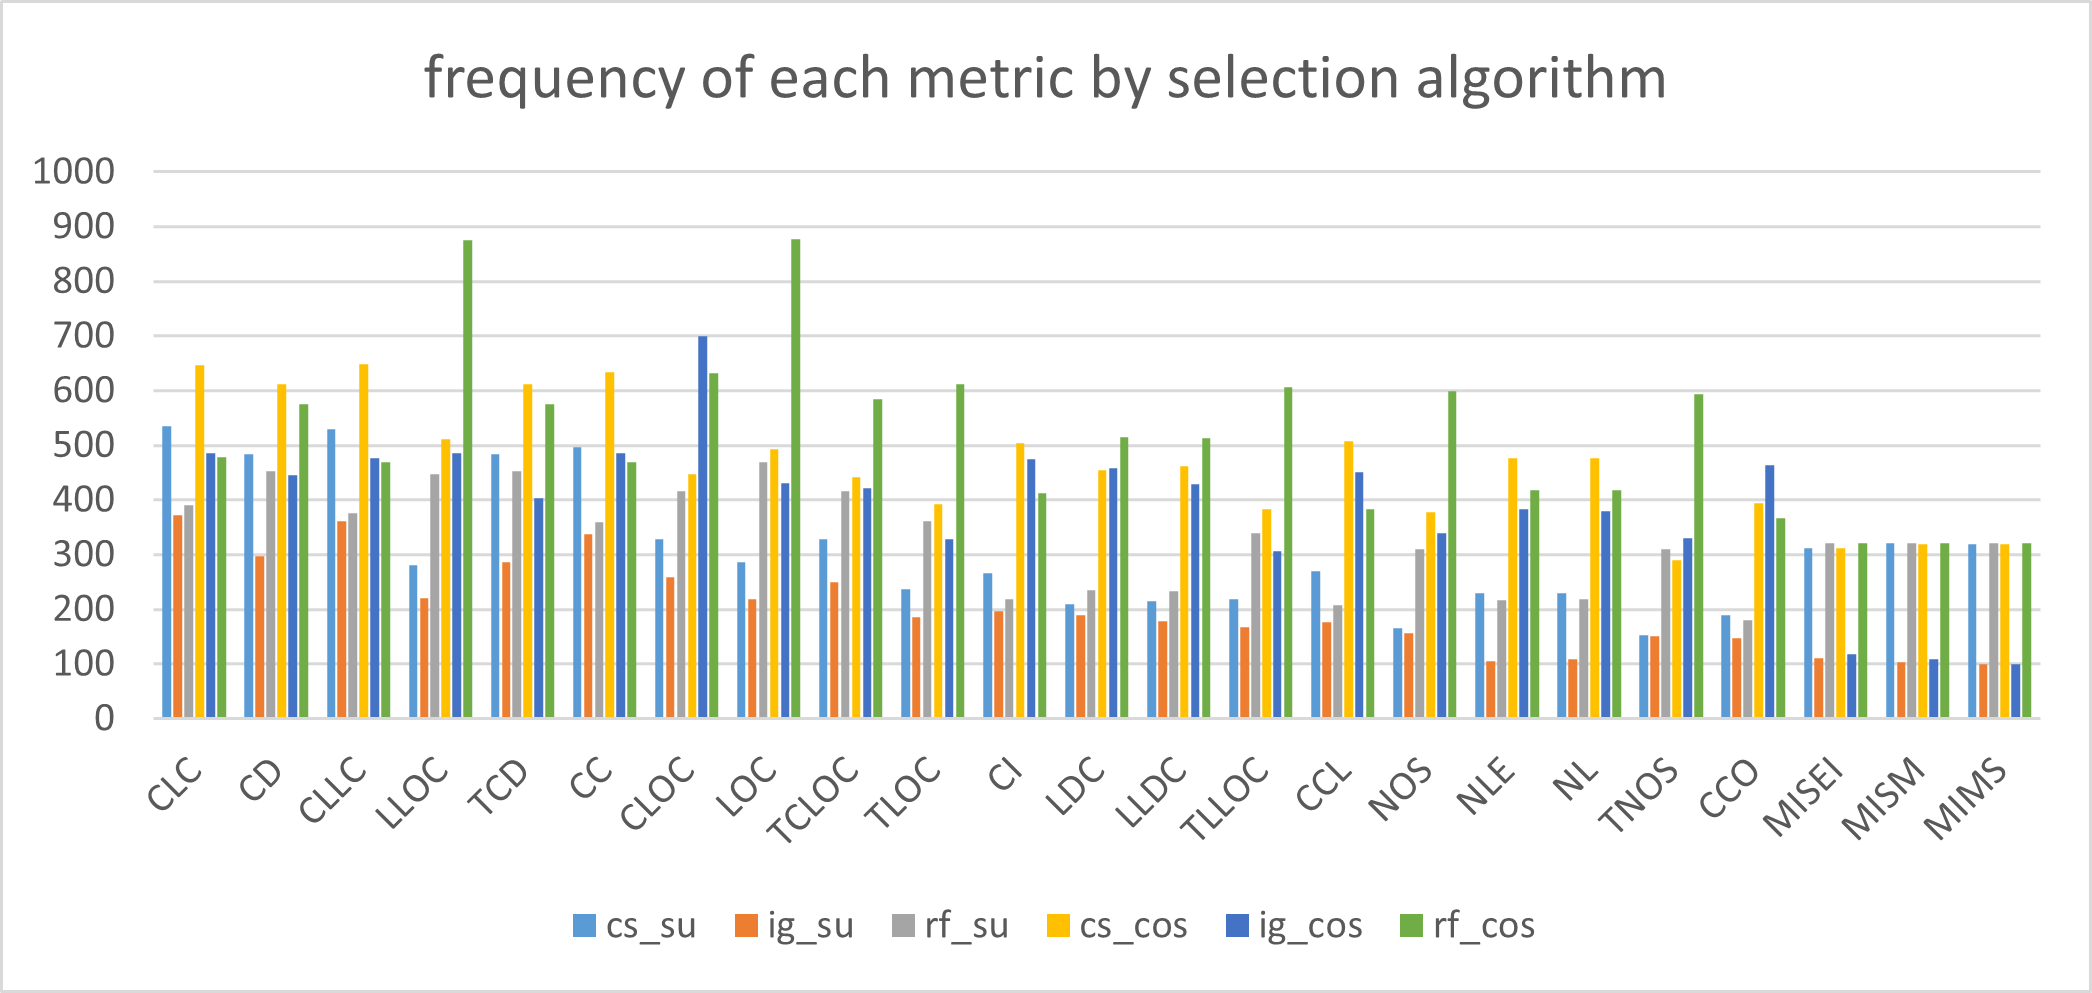
\includegraphics[scale=0.9]{chapters/chapter3/Sections/Research Questions/sections/RQ2/img/frec_by.png} %Change the figure name 
	\setstretch{1} %Interlineado 1
	\captionsetup{labelsep=period, labelfont=bf}
	\caption[Frecuencia de cada métrica \(\beta\) y algoritmo de selección]{Frecuencia de cada métrica \(\beta\) y algoritmo de selección}
 %[Se muestra en el índice]{Se muestra en el pie de figura}
	\label{fig:frecuencyby}
\end{figure}



En la la tabla \ref{table:selected_metrics} se muestra las métricas de código y la tabla \ref{table:cloneMetrics} separa las métricas de clone \cite{ferenc_automatically_2020} las cuales son calculadas a nivel de método y clase.

\input{chapters/chapter3/Sections/Research Questions/sections/RQ2/tables/selected_metrics}

Como se evidencia en la Tabla \ref{table:selected_metrics}, las métricas seleccionadas prioritariamente corresponden al nivel de método, seguidas por las métricas a nivel de clase y, finalmente, las de archivo. Es importante destacar que la cantidad de métricas disponibles a nivel de archivo es considerablemente menor en comparación con las de nivel de método y clase. Paralelamente, según lo indicado en la Tabla \ref{metrics-table}, solo tres métricas - CLOC, LOC y LLOC - están presentes en los tres niveles mencionados. Estas métricas fueron seleccionadas entre las más contribuyentes a los modelos predictivos. Esto subraya la relevancia y eficacia de dichas métricas en la predicción de errores.

\input{chapters/chapter3/Sections/Research Questions/sections/RQ2/tables/clone_metrics}


En la tabla \ref{table:metric_cero_varia} se muestran las métricas que no tienen variación en sus datos, aquellas que contengan aproximadamente un 95\% o más de sus datos con un valor constante. 

 \input{chapters/chapter3/Sections/Research Questions/sections/RQ2/tables/metrics_cero_varia}

De acuerdo con los análisis presentados en las tablas \ref{description-table} y \ref{table:metric_cero_varia}, se observa que, a excepción de la métrica TNOS, todas las demás métricas relacionadas con la violación de reglas presentan poca variación en sus datos (ver tabla \ref{table:smell_metrics}). Este patrón sugiere que dichas métricas podrían no ser particularmente relevantes para el proceso de predicción de errores en el contexto estudiado.

\textit{Advertencia sobre un posible artefacto de conteo.} Una explicación alternativa, no excluyente, para la alta frecuencia de selección de CLOC, LOC y LLOC es un artefacto de conteo: al ser las únicas tres métricas disponibles en los tres niveles de granularidad, tienen estructuralmente el triple de oportunidades de ser seleccionadas que una métrica exclusiva de un solo nivel, y el doble que una disponible en dos niveles. Los datos actuales no permiten distinguir, sin reprocesar los registros de selección normalizando por nivel de granularidad, entre valor predictivo genuino y este efecto de oportunidad; esta verificación se declara como trabajo futuro (Capítulo \ref{cap:conclusion}) y como amenaza a la validez de constructo (Capítulo \ref{cap:discusion}).

\noindent\fbox{%
\parbox{\dimexpr\textwidth-2\fboxsep-2\fboxrule\relax}{%
\textbf{Respuesta RQ2}
   Entre las métricas con mayor contribución se encuentran aquellas calculables en los tres niveles: método, clase y archivo, específicamente CLOC, LOC y LLOC, aunque parte de su preeminencia puede deberse a que tienen más oportunidades de ser seleccionadas. No obstante, según se detalla en la Tabla \ref{table:selected_metrics}, las métricas de código más relevantes para los modelos empleados en la selección de características son, en orden de importancia, aquellas a nivel de método, clase y archivo, respectivamente. En resumen, las métricas más relevantes para la predicción de errores son las métricas de código fuente, seguidas por las métricas de clonación de código, mientras que las métricas de violación de reglas (\textit{code smells}) quedan prácticamente fuera, con la excepción de TNOS.
}%
}
\vspace{12pt}
\section{Tercera pregunta de investigación}


\noindent\fbox{%
\parbox{\dimexpr\textwidth-2\fboxsep-2\fboxrule\relax}{%
\textbf{RQ3} ¿Como influye la variación de los parámetros de entrada a los algoritmos de análisis de relevancia y control de redundancia en los resultados de los modelos de clasificación?%
}%
}
\vspace{12pt}


\section{Estadísticas Descriptivas de FMeasure}

Las estadísticas descriptivas de la columna \textbf{FMeasure} son las siguientes:

\begin{itemize}
    \item Cantidad de registros (count): 13,916
    \item Media (mean): 0.547
    \item Desviación estándar (std): 0.104
    \item Valor mínimo (min): 0.274
    \item Percentil 25\%: 0.488
    \item Mediana (50\%): 0.529
    \item Percentil 75\%: 0.610
    \item Valor máximo (max): 0.844
\end{itemize}

Estos datos nos indican que la media de la medida F es aproximadamente 0.547, con una variabilidad moderada (desviación estándar de 0.104). El rango de los valores de FMeasure va desde 0.274 hasta 0.844.

\section{Correlación entre FMeasure, Rank y \(\beta\)}

A continuación, examinaré la correlación entre las columnas FMeasure, Rank y \(\beta\) para entender cómo se relacionan estas variables entre sí. Posteriormente, representaré visualmente estas relaciones.

\begin{figure}[H]
    \centering
    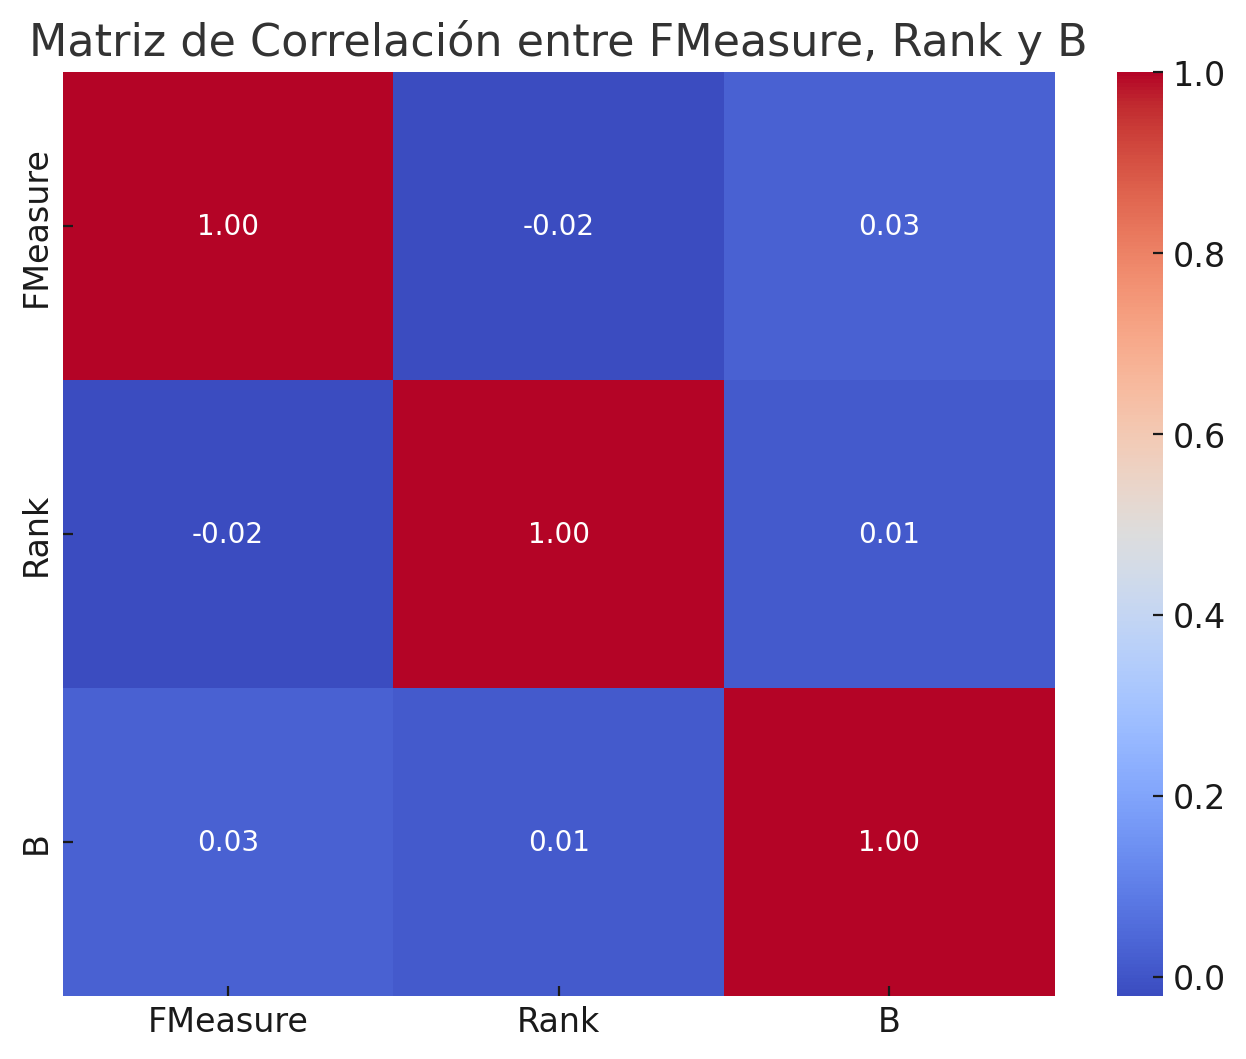
\includegraphics[width=100mm, height=80mm,]{chapters/chapter3/Sections/Research Questions/sections/RQ3/img/matriz.png}
    \setstretch{1} %Interlineado 1
	\captionsetup{labelsep=period, labelfont=bf}
    \caption{Frecuencia de cada métrica \(\beta\) y algoritmo de selección}
    \label{fig:frecuencyby}
\end{figure}

La matriz de correlación entre \textbf{FMeasure}, \textbf{Rank} y \textbf{B} revela lo siguiente:
{
\fontsize{14pt}{14pt}\selectfont
\begin{itemize}
    \item{Correlación entre FMeasure y Rank:} -0.021, lo que indica una correlación negativa muy débil. 
    \item{Correlación entre FMeasure y  \(\beta\):} 0.027, sugiriendo una correlación positiva muy débil. 
    \item{Correlación entre Rank y \(\beta\):} 0.011, lo que implica una correlación positiva casi inexistente.
\end{itemize}
}

Estas correlaciones sugieren que ni \textit{Rank} ni \textit{B} tienen una relación fuerte con \textit{FMeasure}.

Aunque no se observa una correlación fuerte entre los parámetros de entrada y el FMeasure, la Figura \ref{fig:FMeasure_rank_b} ilustra que, generalmente, valores menores de 'Rank' y mayores de 'B' se asocian con mejores resultados de FMeasure. Además, se identifica una tendencia descendente en los valores de FMeasure a medida que aumenta el 'Rank' para los tres valores distintos de 'B' evaluados.

\begin{figure}[H]
    \centering
    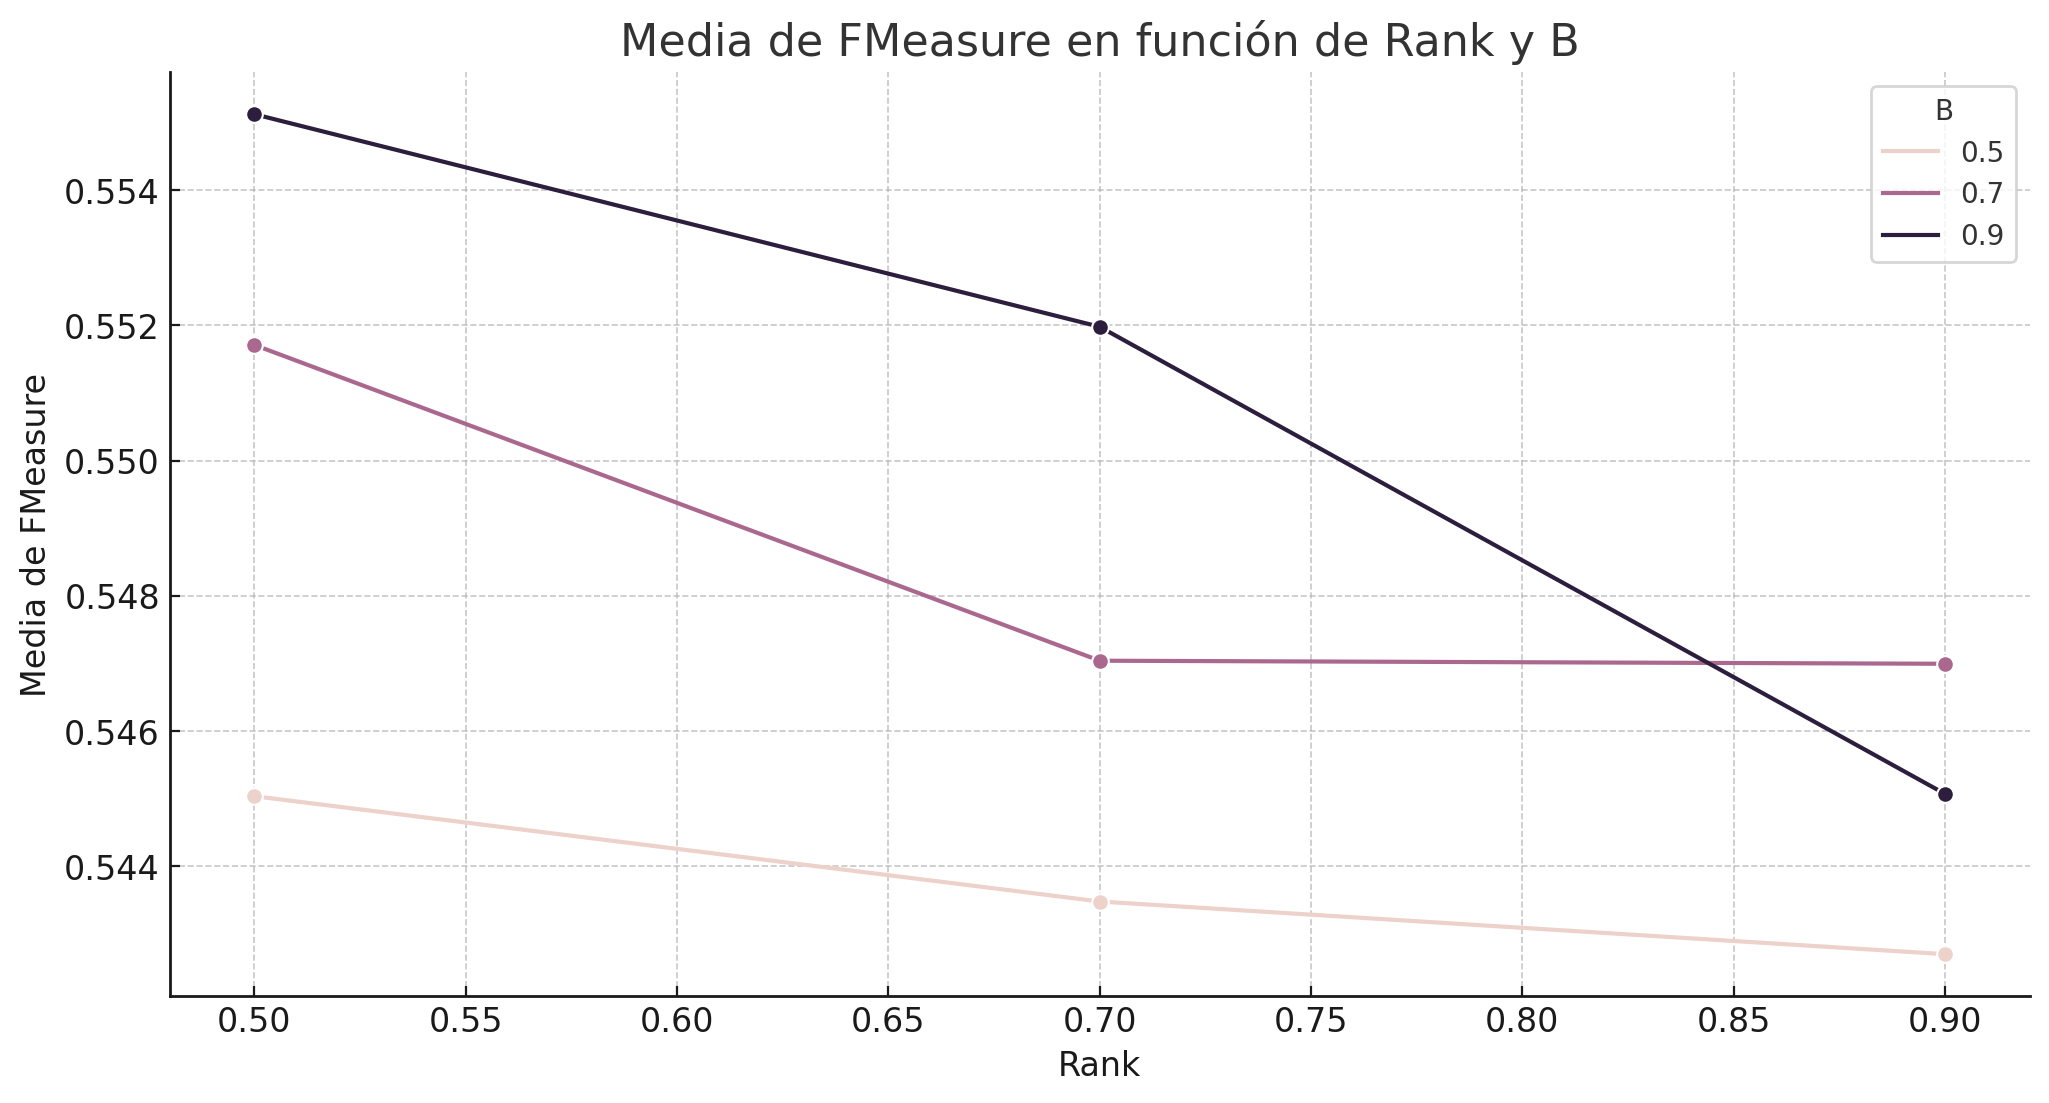
\includegraphics[width=150mm, height=120mm,]{chapters/chapter3/Sections/Research Questions/sections/RQ3/img/medida f en funcion de ran y b.png}
     \setstretch{1} %Interlineado 1
	\captionsetup{labelsep=period, labelfont=bf}
    \caption{Medición basada en rango y $\beta$}
    \label{fig:FMeasure_rank_b}
\end{figure}

En las tablas \ref{table:b_u_c_m}, \ref{table:b_u_c_c} y \ref{table:b_u_c_f} observamos que se obtienen valores similares a los obtenidos en la linea base (\ref{table:original_result_average}) pero con una disminución significativa de las características ingresadas en los modelos de clasificación. 

\noindent\fbox{%
\parbox{\dimexpr\textwidth-2\fboxsep-2\fboxrule\relax}{%
\textbf{Respuesta RQ3} 
En resumen, se observa que los parámetros de entrada utilizados en los algoritmos de análisis de relevancia y control de redundancia no presentan una correlación fuerte con el FMeasure. Sin embargo, se identifica que valores menores de 'Rank' y mayores de \( \beta \)  se asocian, en promedio, con mejores resultados de FMeasure. Paralelamente, se destaca que los algoritmos de selección reducen la cantidad de características ingresadas a los algoritmos, manteniendo o incluso mejorando los valores de FMeasure. Esto sugiere que, a pesar de la diversidad de los resultados, los valores seleccionados fueron eficaces para cumplir su propósito con un conjunto reducido de características.
}%
}
\vspace{12pt}
\section{Cuarta pregunta de investigación}
\label{sec:RQ4}

\noindent\fbox{%
\parbox{\dimexpr\textwidth-2\fboxsep-2\fboxrule\relax}{%
\textbf{RQ4} ¿Cómo influyen los algoritmos de balanceo de clases ROS, RUS y SMOTE en los resultados de los clasificadores?%
}%
}
\vspace{12pt}

\subsection{Desbalance de BugHunter}

La Tabla \ref{table:count_bug_nobug} muestra el número de instancias con error (\textit{bug}) y sin error por proyecto y nivel. En la mayoría de los proyectos predominan las instancias sin error, aunque la proporción varía considerablemente entre proyectos y niveles.

\input{chapters/chapter3/Sections/Research Questions/sections/RQ4/tables/count_bug_nobug}

La Tabla \ref{tab:desbalance} resume esta distribución tras binarizar el atributo \textit{Number of Bugs}. El desequilibrio de BugHunter es moderado si se compara con los conjuntos clásicos de PFS ---como NASA o PROMISE, donde la clase con error suele representar menos del 10\,\% de las instancias \cite{8494821}---: la mediana de instancias \textit{bug} entre los 15 proyectos es del 28,1\,\% a nivel de método, 41,1\,\% a nivel de clase y 42,7\,\% a nivel de archivo, y en tres proyectos (\textit{hazelcast}, \textit{MapDB} y \textit{elasticsearch}) la clase \textit{bug} llega a ser mayoritaria a nivel de archivo. Esta característica es consecuencia directa del diseño de BugHunter, que solo incluye elementos de código efectivamente afectados por errores. El caso más desequilibrado es \textit{oryx} (razón no-bug:bug de 7,6:1 a nivel de método), lo que debe tenerse presente al interpretar su desempeño, el más alto del estudio.

\begin{table}[H]
\centering
\caption{Proporción de instancias con error (\textit{bug}) por nivel de granularidad, sobre los 15 proyectos individuales}
\label{tab:desbalance}
\resizebox{\textwidth}{!}{%
\begin{tabular}{lccccc}
\toprule
Nivel & Mediana & Mín. (proyecto) & Máx. (proyecto) & ``All'' & Razón mediana \\
      & \% bug  &                 &                 & \% bug  & no-bug:bug \\
\midrule
Método  & 28,1 & 11,7 (\textit{oryx}) & 42,2 (\textit{hazelcast}) & 37,0 & 2,6:1 \\
Clase   & 41,1 & 12,5 (\textit{oryx}) & 53,0 (\textit{hazelcast}) & 48,6 & 1,4:1 \\
Archivo & 42,7 & 13,2 (\textit{oryx}) & 55,2 (\textit{hazelcast}) & 50,7 & 1,3:1 \\
\bottomrule
\end{tabular}}
\end{table}

\subsection{Efecto del balanceo sobre el \textit{F-measure} ponderado}

La Tabla \ref{tab:balance} resume el \textit{F-measure} promedio de las 13.916 ejecuciones agrupadas por técnica de balanceo, comparando el conjunto de entrenamiento original con su versión balanceada (el conjunto de prueba nunca se balancea). Con las tres técnicas, balancear el conjunto de entrenamiento no mejoró el \textit{F-measure} promedio respecto a entrenar con la distribución original. El efecto fue más marcado en RUS, cuya eliminación de instancias de la clase mayoritaria redujo la información disponible para el entrenamiento. Las desviaciones estándar fueron similares entre ambas condiciones (0,108 sin balancear; 0,104, 0,082 y 0,105 balanceando con ROS, RUS y SMOTE, respectivamente).

\begin{table}[H]
\centering
\caption{\textit{F-measure} promedio según técnica de balanceo (13.916 ejecuciones)}
\label{tab:balance}
\begin{tabular}{lccc}
\toprule
Técnica & Sin balancear & Balanceado & $\Delta$ \\
\midrule
ROS   & 0,555 & 0,548 & $-0{,}007$ \\
RUS   & 0,555 & 0,524 & $-0{,}031$ \\
SMOTE & 0,555 & 0,548 & $-0{,}007$ \\
\bottomrule
\end{tabular}
\end{table}

\begin{figure}[H]
    \centering
    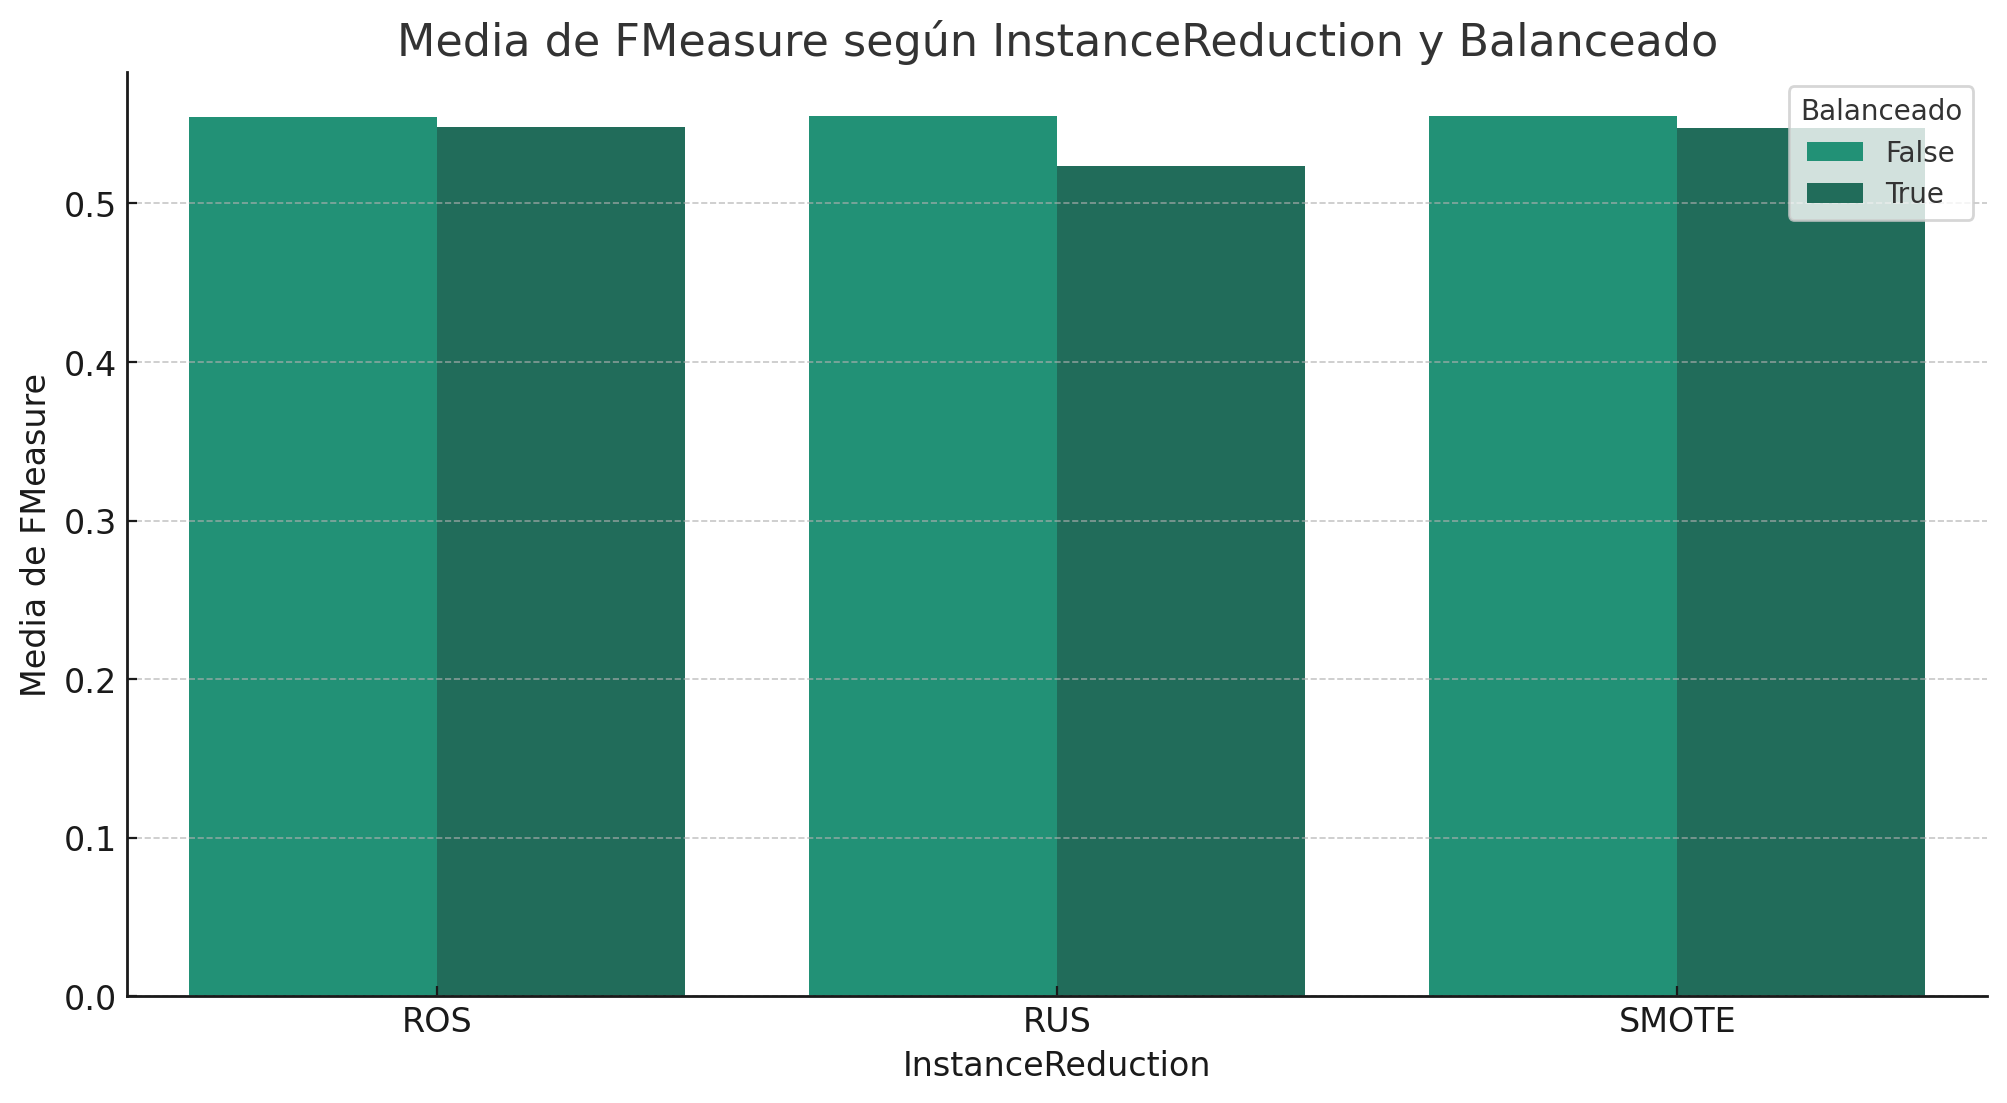
\includegraphics[width=150mm, height=120mm,]{chapters/chapter3/Sections/Research Questions/sections/RQ4/img/InstancereductionBalanceado.png}
     \setstretch{1} %Interlineado 1
	\captionsetup{labelsep=period, labelfont=bf}
    \caption{\textit{F-measure} medio según algoritmo de balanceo y condición de balanceo del entrenamiento}
    \label{fig:ROSRUSSMOTE}
\end{figure}

Para contrastar formalmente esta observación se aplicó una prueba de Wilcoxon de rangos con signo \cite{wilcoxon1945}, pareada por conjunto de datos, sobre el mejor \textit{F-measure} balanceado frente al mejor sin balancear de cada uno de los 16 conjuntos por nivel, complementada con el tamaño de efecto $\delta$ de Cliff \cite{cliff1993}. A nivel de método la diferencia resultó estadísticamente significativa a favor de la versión sin balancear ($p = 0{,}012$), aunque con un tamaño de efecto insignificante ($\delta = 0{,}07$); a nivel de clase ($p = 0{,}48$) y de archivo ($p = 0{,}86$) no se detectaron diferencias significativas, y al agrupar los tres niveles el resultado quedó en el límite de la significancia ($p = 0{,}052$). En los cuatro casos el tamaño de efecto fue insignificante ($|\delta| < 0{,}15$).

\subsection{Efecto del balanceo sobre la clase minoritaria}

Estas cifras deben interpretarse con cautela. Las medias de la Tabla \ref{tab:balance} se analizaron de forma descriptiva sobre todas las ejecuciones, mientras que la prueba estadística se aplicó a la mejor configuración por proyecto, sujeta a un sesgo de selección optimista. Además, el \textit{F-measure} agregado pondera ambas clases por su frecuencia, de modo que la contribución de la clase de interés práctico (\textit{bug}) queda diluida. Este efecto está acotado por el desequilibrio moderado de BugHunter (Tabla \ref{tab:desbalance}), pero no desaparece: la línea base del conjunto ``All'' a nivel de método (Tabla \ref{tab:porclase}) muestra que un \textit{F-measure} ponderado de 0,565 convive con un \textit{F-measure} de 0,356 para la clase \textit{bug} y un MCC cercano a cero.

Dos fuentes de evidencia permiten ir más allá de la métrica agregada. La primera son las matrices de confusión que Weka entrega para las mejores configuraciones a nivel de método (Tabla \ref{table:weka_method_smote_b}), a partir de las cuales se calculan el \textit{F-measure} de la clase \textit{bug} y el MCC (Sección \ref{sec:validacion_flujos}). Sobre los 16 conjuntos, entrenar con SMOTE reduce la mediana del \textit{F-measure} ponderado de 0,600 a 0,581, pero eleva la mediana del \textit{F-measure} de la clase \textit{bug} de 0,280 a 0,334; en MCC, en cambio, la diferencia es pequeña y de signo opuesto (0,070 frente a 0,056). Debe notarse que estas configuraciones fueron elegidas por su \textit{F-measure} ponderado y no por su desempeño en la clase minoritaria. La segunda fuente, más completa, es el análisis de sensibilidad (Sección \ref{sec:sensibilidad}), que almacena las métricas por clase para sus 28.440 ejecuciones y muestra que el balanceo mejora de forma consistente el \textit{F-measure} de la clase \textit{bug} y el MCC en los tres clasificadores evaluados, aun cuando el \textit{F-measure} ponderado apenas varía.

\subsection{¿Qué técnica de balanceo es más efectiva?}

La respuesta depende del objetivo. La Tabla \ref{tab:balanceo_tecnica} resume, sobre las ejecuciones del análisis de sensibilidad en los 15 proyectos individuales, la mediana de cada métrica según la técnica de balanceo. Con \textit{Random Forest} y XGBoost, RUS obtiene el mayor \textit{F-measure} de la clase \textit{bug} y el mejor MCC, pero también el menor \textit{F-measure} ponderado: al eliminar instancias de la clase mayoritaria, el modelo predice defectos con más frecuencia, lo que mejora su detección a costa de más falsos positivos. ROS y SMOTE ofrecen un compromiso intermedio, con mejoras más moderadas en la clase \textit{bug} y una pérdida menor en el agregado. Con la SVM lineal, las tres técnicas producen mejoras similares y grandes en la clase \textit{bug}, porque sin balanceo este clasificador casi no predice defectos. Por tanto, si el objetivo es detectar la mayor cantidad posible de código defectuoso, RUS es la técnica más efectiva; si se busca preservar el desempeño global, ROS o SMOTE son preferibles.

\begin{table}[H]
\centering
\caption{Mediana del desempeño por técnica de balanceo en el análisis de sensibilidad (15 proyectos individuales, todas las configuraciones)}
\label{tab:balanceo_tecnica}
\begin{tabular}{llccc}
\toprule
Clasificador & Balanceo & \textit{F-measure} ponderado & \textit{F-measure} bug & MCC \\
\midrule
RF   & Ninguno & 0,537 & 0,325 & $-0{,}015$ \\
RF   & ROS     & 0,529 & 0,356 & $-0{,}008$ \\
RF   & RUS     & 0,513 & 0,417 & 0,009 \\
RF   & SMOTE   & 0,532 & 0,343 & $-0{,}013$ \\
\midrule
XGB  & Ninguno & 0,540 & 0,318 & 0,003 \\
XGB  & ROS     & 0,537 & 0,367 & 0,001 \\
XGB  & RUS     & 0,524 & 0,427 & 0,027 \\
XGB  & SMOTE   & 0,542 & 0,346 & $-0{,}004$ \\
\midrule
SVM  & Ninguno & 0,551 & 0,171 & 0,038 \\
SVM  & ROS     & 0,562 & 0,423 & 0,086 \\
SVM  & RUS     & 0,558 & 0,426 & 0,081 \\
SVM  & SMOTE   & 0,565 & 0,425 & 0,087 \\
\bottomrule
\end{tabular}
\end{table}

Las medianas de MCC cercanas a cero reflejan que la tabla incluye todas las configuraciones de selección, también las peores; las mejoras sobre la mejor configuración de cada proyecto se presentan en la Tabla \ref{tab:sensibilidad}.

\noindent\fbox{%
\parbox{\dimexpr\textwidth-2\fboxsep-2\fboxrule\relax}{%
\textbf{Respuesta RQ4}
Balancear solo el conjunto de entrenamiento con ROS, RUS o SMOTE no mejora el \textit{F-measure} ponderado cuando el conjunto de prueba conserva la distribución real de clases; RUS lo empeora de forma más marcada ($-0{,}031$). La diferencia entre las mejores configuraciones con y sin balanceo tiene un tamaño de efecto insignificante ($|\delta| < 0{,}15$) en los tres niveles. Sin embargo, el balanceo sí desplaza el desempeño hacia la clase de interés práctico: aumenta el \textit{F-measure} de la clase \textit{bug} y, en el análisis de sensibilidad, también el MCC. La conclusión de RQ4 depende, por tanto, de la métrica de evaluación empleada. Entre las técnicas, RUS maximiza la detección de defectos y ROS y SMOTE preservan mejor el desempeño global.
}%
}
\vspace{12pt}

\section{Quinta pregunta de investigación}

Nuestra ultima pregunta de investigación va enfocada a diferenciar los resultados entre el conjunto de datos resumen (unión de todos los proyectos en cada nivel) y los resultados individuales por proyecto.

\noindent\fbox{%
\parbox{\dimexpr\textwidth-2\fboxsep-2\fboxrule\relax}{%
\textbf{RQ5} ¿Que diferencias existen entre el proyecto resumen y los proyectos individuales en los resultados obtenidos en las preguntas anteriores?%
}%
}
\vspace{12pt}

El conjunto de datos All esta diseñado a partir de la unión de todos los conjuntos de datos en el mismo nivel de los 15 proyectos seleccionados, por ende existe un conjunto All para cada nivel método, clase y archivo. Contiene una mayor cantidad de registros que todos los proyectos individuales por su origen como se puede observar en la tabla \ref{table:count_bug_nobug}.

Iniciando con el análisis de los resultados base obtenidos en la sección \ref{sec:datasetoriginal}, observamos en las tablas \ref{table:original_result_weka_method_result}, \ref{table:original_result_weka_class_result} y \ref{table:original_result_weka_file_result} que en ninguno de los 3 niveles se obtienen los mejores resultados de F-measure para el proyecto All, pero tampoco siendo los peores.

\input{chapters/chapter3/Sections/Research Questions/sections/RQ5/tables/min_max_all}

Este escenario se observa consistentemente en respuesta a la pregunta de investigación RQ1 (véase Sección \ref{sec:RQ1}), como se ilustra en las Tablas \ref{table:b_u_c_m}, \ref{table:b_u_c_c}, y \ref{table:b_u_c_f}. A pesar de implementar la selección de características y el balanceo de clases, los resultados no alcanzan un nivel óptimo de rendimiento. Este fenómeno sugiere que la amalgama de métricas de código procedentes de diversos proyectos, los cuales pueden variar significativamente en metodologías de desarrollo, equipos de programación y objetivos, no contribuye necesariamente a la mejora de la precisión de los clasificadores. Se infiere que un análisis a nivel de proyecto individual es más fructífero, ya que los errores detectados en cada proyecto podrían estar intrínsecamente relacionados con aspectos específicos de desarrollo y estructura propios del software en cuestión. Por consiguiente, la expansión del volumen de datos mediante la combinación de métricas de diferentes proyectos no garantiza una mejora en los resultados, según se desprende de nuestro análisis.

\noindent\fbox{%
\parbox{\dimexpr\textwidth-2\fboxsep-2\fboxrule\relax}{%
\textbf{Respuesta RQ5} 
 El proyecto resumen cuenta con una mayor cantidad de registros unificando los diferentes proyectos, pero aun así esto no conlleva a la mejora de los resultados de los clasificadores en ninguna de los escenarios analizados: conjunto de datos original, selección de características y balanceo de clases. Por tanto, concluimos que se obtienen mejores resultados entrenando los clasificadores con métricas de software individuales, dado que cada software tiene sus aspectos específicos de desarrollo 
}%
}
\vspace{12pt}

\section{Validación cruzada entre herramientas: Weka y \textit{scikit-learn}}
\label{sec:validacion_flujos}

El estudio principal combina dos herramientas: la selección de características, la partición estratificada 67/33 y el balanceo del entrenamiento se realizan en Python, mientras que la clasificación con \textit{Random Forest} se ejecuta en Weka en modalidad \textit{Supplied test set} (Sección \ref{sec:RQ1}). El análisis de sensibilidad (Sección \ref{sec:sensibilidad}), en cambio, se ejecuta completamente en \textit{scikit-learn}. Para verificar que ambos flujos son intercambiables, se compararon las 32 mejores configuraciones a nivel de método registradas en Weka ---16 conjuntos, sin balancear y con SMOTE (Tabla \ref{table:weka_method_smote_b})--- con la configuración idéntica (proyecto, esquema, \textit{Rank}, $\beta$ y balanceo) del análisis de sensibilidad ejecutado con \textit{Random Forest} en \textit{scikit-learn}. La comparación no requiere reejecutar modelos y se implementó en el \textit{script} \texttt{validar\_weka\_vs\_sklearn.py}.

\begin{table}[H]
\caption{\label{table:weka_method_smote_b}Mejor resultado por proyecto a nivel de método en Weka (\textit{Supplied test set}), sin balancear y balanceando el entrenamiento con SMOTE, con su matriz de confusión (clase positiva: \textit{bug})}
\resizebox{\textwidth}{!}{
\begin{tabular}{lllllllllllll}
\hline
\multicolumn{13}{c}{\textbf{SMOTE}}                                                                                                                                                                               \\\hline 
\multicolumn{13}{c}{\textbf{MÉTODO}}                                                                                                                                                                       \\\hline
\textbf{Proyecto}               & \textbf{Precisión} & \textbf{Recall} & \textbf{F-measure} & \textbf{Variación} & \textbf{Rank} & \textbf{$\beta$} & \textbf{Esquema} & \textbf{TP} & \textbf{TN} & \textbf{FN} & \textbf{FP} & \textbf{Balanceado} \\\hline
oryx                           & 0,825              & 0,859           & 0,838             & 0,029              & 0.7           & 0.7        & CS\_SU                  & 5           & 238         & 28          & 12          & No               \\
                           & 0,82               & 0,799           & 0,809             &                    & 0.7           & 0.7        & CS\_SU                  & 9           & 217         & 24          & 33          & Sí                \\
antlr4                         & 0,8                & 0,795           & 0,797             & 0,026              & 0.5           & 0.9        & RF\_COS                 & 15          & 221         & 29          & 32          & Sí                \\
                         & 0,746              & 0,801           & 0,771             &                    & 0.5           & 0.9        & RF\_COS                 & 3           & 235         & 41          & 18          & No               \\
BroadleafCommerce              & 0,757              & 0,77            & 0,762             & 0                  & 0.5           & 0.5        & CS\_COS                 & 196         & 1160        & 245         & 159         & Sí                \\
              & 0,76               & 0,78            & 0,762             &                    & 0.5           & 0.5        & CS\_COS                 & 169         & 1203        & 272         & 116         & No               \\
mct                            & 0,706              & 0,694           & 0,7               & 0,016              & 0.7           & 0.7        & IG\_SU                  & 4           & 21          & 5           & 6           & No               \\
                            & 0,716              & 0,667           & 0,684             &                    & 0.7           & 0.7        & IG\_SU                  & 5           & 19          & 4           & 8           & Sí                \\
junit                          & 0,676              & 0,722           & 0,694             & 0,02               & 0.9           & 0.9        & IG\_COS                 & 6           & 116         & 31          & 16          & No               \\
                          & 0,668              & 0,68            & 0,674             &                    & 0.9           & 0.9        & IG\_COS                 & 8           & 107         & 29          & 25          & Sí                \\
netty                          & 0,638              & 0,684           & 0,653             & 0,013              & 0.9           & 0.9        & RF\_COS                 & 234         & 2823        & 961         & 452         & No               \\
                          & 0,63               & 0,654           & 0,64              &                    & 0.9           & 0.9        & RF\_COS                 & 298         & 2624        & 897         & 651         & Sí                \\
titan                          & 0,634              & 0,663           & 0,645             & 0,052              & 0.7           & 0.7        & CS\_SU                  & 25          & 199         & 70          & 44          & No               \\
                          & 0,607              & 0,583           & 0,593             &                    & 0.7           & 0.7        & CS\_SU                  & 34          & 163         & 61          & 80          & Sí                \\
ceylon-ide-eclipse             & 0,601              & 0,657           & 0,62              & 0,008              & 0.7           & 0.7        & IG\_COS                 & 33          & 486         & 185         & 86          & No               \\
             & 0,6                & 0,629           & 0,612             &                    & 0.7           & 0.7        & IG\_COS                 & 46          & 451         & 172         & 121         & Sí                \\
mcMMO                          & 0,577              & 0,604           & 0,581             & 0,016              & 0.7           & 0.9        & IG\_COS                 & 48          & 225         & 118         & 61          & No               \\
                          & 0,561              & 0,569           & 0,565             &                    & 0.7           & 0.9        & IG\_COS                 & 62          & 195         & 104         & 91          & Sí                \\
all                            & 0,567              & 0,59            & 0,573             & 0,004              & 0.9           & 0.9        & RF\_COS                 & 5958        & 25034       & 13449       & 8055        & No               \\
                            & 0,563              & 0,579           & 0,569             &                    & 0.9           & 0.9        & RF\_COS                 & 6610        & 23775       & 12797       & 9314        & Sí                \\
elasticsearch                  & 0,567              & 0,586           & 0,571             & 0,014              & 0.5           & 0.9        & CS\_COS                 & 2189        & 7768        & 4340        & 2708        & No               \\
                  & 0,555              & 0,559           & 0,557             &                    & 0.5           & 0.9        & CS\_COS                 & 2593        & 6920        & 3936        & 3556        & Sí                \\
orientdb                       & 0,557              & 0,598           & 0,569             & 0,017              & 0.7           & 0.5        & RF\_COS                 & 320         & 2284        & 1154        & 598         & No               \\
                       & 0,551              & 0,553           & 0,552             &                    & 0.7           & 0.5        & RF\_COS                 & 492         & 1915        & 982         & 967         & Sí                \\
hazelcast                      & 0,551              & 0,559           & 0,553             & 0,003              & 0.7           & 0.7        & CS\_COS                 & 3206        & 7202        & 4658        & 3562        & No               \\
                      & 0,549              & 0,552           & 0,55              &                    & 0.7           & 0.7        & CS\_COS                 & 3478        & 6807        & 4386        & 3957        & Sí                \\
neo4j                          & 0,538              & 0,577           & 0,552             & 0,007              & 0.9           & 0.7        & RF\_COS                 & 205         & 1642        & 843         & 511         & No               \\
                          & 0,538              & 0,553           & 0,545             &                    & 0.9           & 0.7        & RF\_COS                 & 268         & 1502        & 780         & 651         & Sí                \\
Android-Universal-Image-Loader & 0,545              & 0,543           & 0,544             & 0,025              & 0.5           & 0.7        & IG\_SU                  & 16          & 54          & 29          & 30          & Sí                \\
 & 0,508              & 0,535           & 0,519             &                    & 0.5           & 0.7        & IG\_SU                  & 10          & 59          & 35          & 25          & No               \\
MapDB                          & 0,529              & 0,557           & 0,538             & 0,02               & 0.7           & 0.5        & IG\_SU                  & 54          & 274         & 159         & 102         & No               \\
                          & 0,518              & 0,518           & 0,518             &                    & 0.7           & 0.5        & IG\_SU                  & 71          & 234         & 142         & 142         & Sí               
\end{tabular}
}
\end{table}

Los resultados son los siguientes:

\begin{itemize}
    \item \textbf{Particiones idénticas.} El tamaño del conjunto de prueba coincide en las 32 configuraciones, lo que confirma que ambos flujos evalúan sobre la misma partición estratificada.
    \item \textbf{\textit{F-measure} ponderado.} La diferencia absoluta mediana entre herramientas es de 0,010, y 23 de las 32 configuraciones difieren en 0,02 o menos. Las diferencias mayores (hasta 0,060) se concentran en los proyectos con conjuntos de prueba pequeños, como \textit{mct} (36 instancias) y \textit{Android-Universal-Image-Loader} (129), donde unas pocas predicciones distintas alteran la métrica. Weka obtiene un valor ligeramente superior en 24 de las 32 configuraciones (diferencia media de 0,010), lo esperable dado que estas configuraciones fueron seleccionadas como las mejores dentro del propio Weka.
    \item \textbf{Métricas por clase.} Con la matriz de confusión de Weka se calcularon el \textit{F-measure} de la clase \textit{bug} y el MCC. Ambas herramientas reproducen el mismo patrón frente al balanceo: con SMOTE, el \textit{F-measure} ponderado apenas varía (medianas de 0,600 a 0,581 en Weka y de 0,583 a 0,578 en \textit{scikit-learn}), mientras que el \textit{F-measure} de la clase \textit{bug} aumenta (de 0,280 a 0,334 en Weka y de 0,250 a 0,293 en \textit{scikit-learn}). En MCC, en estas configuraciones elegidas por su \textit{F-measure} ponderado, la variación es pequeña y negativa en ambas herramientas.
\end{itemize}

En conjunto, la diferencia de herramienta introduce una variación del orden de 0,01 en el \textit{F-measure} ponderado, un orden de magnitud menor que las diferencias entre proyectos, y no altera el sentido de ninguna de las conclusiones. Esto permite comparar directamente los resultados del estudio principal (Weka) con los del análisis de sensibilidad (\textit{scikit-learn}).


\section{Análisis de sensibilidad: clasificadores adicionales y línea base unificada}
\label{sec:sensibilidad}

El estudio principal presenta dos limitaciones de diseño: utiliza un único clasificador y su línea base se calculó con una herramienta y un esquema de validación distintos (Weka con validación cruzada de 10 particiones) de los del resto de los experimentos (partición 67/33). Para mitigarlas se ejecutó un análisis de sensibilidad que repite el flujo completo sobre los 48 conjuntos proyecto-nivel con tres clasificadores de paradigmas distintos: \textit{Random Forest} como referencia, XGBoost \cite{chen2016} (\textit{boosting} de gradiente) y una SVM lineal \cite{cortes1995} con estandarización previa (Sección \ref{sec:clasificadores_mt}). Los tres clasificadores comparten exactamente la misma partición estratificada 67/33, con semilla fija, en cada conjunto, lo que permite comparaciones pareadas. Se reutilizan los subconjuntos de métricas obtenidos en la selección de características, el balanceo (ROS, RUS y SMOTE) se aplica solo al entrenamiento, y de cada una de las 28.440 ejecuciones (9.480 por clasificador) se almacenan tanto las métricas agregadas como las métricas por clase (\textit{F-measure} de la clase \textit{bug}, MCC y AUC-ROC). El experimento se ejecutó en \textit{scikit-learn}; XGBoost se aceleró en una GPU NVIDIA RTX 3060. Ninguno de los tres clasificadores fue ajustado mediante búsqueda de hiperparámetros.

La semilla fija es una decisión deliberada: permite comparar los distintos esquemas de selección, técnicas de balanceo y clasificadores sobre exactamente la misma división de los datos. Implica, no obstante, que el análisis no promedia sobre múltiples particiones aleatorias, lo que se discute como amenaza a la validez de conclusión en el Capítulo \ref{cap:discusion}.

\subsection{Línea base unificada}

Recalculada con \textit{Random Forest} bajo el mismo esquema \textit{holdout} estratificado 67/33 de \textit{scikit-learn} (todas las características, sin balanceo), la línea base promedia 0,62 a nivel de método, 0,52 a nivel de clase y 0,52 a nivel de archivo, frente a 0,63, 0,50 y 0,50 de la línea base Weka con validación cruzada (Tabla \ref{table:original_result_average}). Las diferencias, de a lo sumo 0,02, indican que el factor de confusión introducido por el cambio de herramienta y de esquema de validación no altera las conclusiones, en línea con la validación de la Sección \ref{sec:validacion_flujos}. En el conjunto ``All'' a nivel de método, el desglose por clase de esta línea base (\textit{F-measure} de la clase \textit{bug} de 0,360, MCC de 0,069 y AUC-ROC de 0,546) coincide estrechamente con el obtenido en Weka (Tabla \ref{tab:porclase}), lo que corrobora ambas mediciones de forma independiente.

\subsection{Generalización entre clasificadores}

La Tabla \ref{tab:sensibilidad} resume las diferencias pareadas sobre los 15 proyectos individuales. Emergen tres patrones.

\textbf{Selección de características (RQ1).} La selección de características no solo conserva, sino que mejora el \textit{F-measure} ponderado en los tres clasificadores (mediana de $+0{,}001$ a $+0{,}041$), con mejora en 14 o 15 de los 15 proyectos en ocho de las nueve combinaciones de clasificador y nivel (9 de 15 para la SVM lineal a nivel de archivo) y $p<0{,}01$ en la prueba de Wilcoxon en todos los casos. Las reducciones medianas de características van del 31\,\% al 82\,\%. El hallazgo de RQ1 no es, por tanto, específico de \textit{Random Forest}.

\textbf{Balanceo de clases (RQ4).} El efecto del balanceo depende del clasificador y, sobre todo, de la métrica. En el \textit{F-measure} ponderado, el balanceo no aporta en \textit{Random Forest} (consistente con RQ4), aporta marginalmente en XGBoost y mejora de forma significativa en la SVM lineal. En las métricas por clase, en cambio, el balanceo mejora la detección de la clase \textit{bug} de manera consistente en los tres clasificadores: el \textit{F-measure} de la clase \textit{bug} aumenta con una mediana de $+0{,}031$ a $+0{,}317$, con mejora en 12 a 15 de los 15 proyectos y $p<0{,}05$ en todos los casos, y el MCC aumenta con una mediana de $+0{,}013$ a $+0{,}055$. Es decir, el resultado nulo de RQ4 es en gran medida un artefacto de la métrica agregada: balancear el entrenamiento sí mejora la capacidad del modelo para identificar código defectuoso, a costa de la clase mayoritaria, y ese intercambio queda oculto en el \textit{F-measure} ponderado.

\textbf{Conjunto unificado (RQ5).} El conjunto ``All'' no obtuvo el mejor resultado con ningún clasificador ni nivel (puestos 7 a 15 de 16 en \textit{F-measure} ponderado y 6 a 13 de 16 en MCC), por lo que la conclusión de RQ5 también se generaliza, incluso bajo una métrica insensible al desequilibrio.

Las diferencias globales entre clasificadores fueron pequeñas (mediana pareada de a lo sumo 0,023 en el mejor \textit{F-measure} ponderado, a favor de la SVM lineal y de XGBoost sobre \textit{Random Forest}). Sin embargo, la SVM lineal sin balanceo tiende fuertemente a la clase mayoritaria (mediana de \textit{F-measure} de la clase \textit{bug} de 0,143 a nivel de método), lo que refuerza la necesidad de leer las métricas por clase junto al agregado.

\begin{table}[H]
\centering
\caption{Análisis de sensibilidad por clasificador: mediana de las diferencias pareadas sobre los 15 proyectos (sel. = mejor esquema de selección frente a todas las características; bal. = mejor entrenamiento balanceado frente a sin balancear) y puesto de ``All'' entre los 16 conjuntos por mejor \textit{F-measure} ponderado}
\label{tab:sensibilidad}
\begin{tabular}{llccccc}
\toprule
Clasificador & Nivel & $\Delta F$ sel. & $\Delta F$ bal. & $\Delta F_{1}$ bug bal. & $\Delta$MCC bal. & ``All'' \\
\midrule
RF  & Método  & +0,014 & $-0{,}001$ & +0,108 & +0,036 & 9/16 \\
RF  & Clase   & +0,028 & +0,002   & +0,072 & +0,026 & 12/16 \\
RF  & Archivo & +0,033 & +0,011   & +0,040 & +0,021 & 12/16 \\
XGB & Método  & +0,014 & +0,005   & +0,135 & +0,045 & 11/16 \\
XGB & Clase   & +0,031 & +0,004   & +0,066 & +0,025 & 7/16 \\
XGB & Archivo & +0,041 & +0,012   & +0,031 & +0,027 & 7/16 \\
SVM & Método  & +0,006 & +0,024   & +0,317 & +0,055 & 15/16 \\
SVM & Clase   & +0,018 & +0,009   & +0,155 & +0,013 & 13/16 \\
SVM & Archivo & +0,001 & +0,033   & +0,206 & +0,041 & 13/16 \\
\bottomrule
\end{tabular}
\end{table}


\section{Piloto exploratorio: modelos de lenguaje de gran escala sobre métricas de BugHunter}
\label{sec:piloto_llm}

Como se discutió en el Capítulo \ref{cap4}, los enfoques basados en modelos de lenguaje de gran escala (LLM) para la predicción de defectos operan, en su mayoría, sobre el código fuente, que BugHunter no incluye. La única forma de aplicar un LLM directamente sobre este conjunto de datos es serializar las métricas de cada instancia como texto \cite{hegselmann2023tabllm}. Este piloto evalúa, de forma exploratoria, si un LLM de propósito general clasifica instancias de BugHunter como defectuosas o no defectuosas mejor o peor que \textit{Random Forest} entrenado con las mismas métricas.

\subsection{Diseño}

\begin{itemize}
    \item \textbf{Datos.} Tres proyectos de tamaño y desequilibrio distintos (\textit{oryx}, \textit{antlr4} y \textit{netty}) en los tres niveles de granularidad, con la misma partición estratificada 67/33 y semilla fija del análisis de sensibilidad. De cada conjunto de prueba se extrae una muestra estratificada de hasta 150 instancias, lo que totaliza 1.296 instancias.
    \item \textbf{Características.} Las 10 métricas más relevantes según la Ganancia de Información, calculada exclusivamente sobre el conjunto de entrenamiento para evitar la fuga de información hacia la prueba (6 métricas a nivel de archivo, donde no hay más disponibles).
    \item \textbf{Serialización y \textit{prompt}.} Cada instancia se serializa como una lista \textit{nombre=valor} de sus métricas. El \textit{prompt} describe la tarea, el nivel de granularidad y la proporción de instancias defectuosas del proyecto, y exige una respuesta en formato JSON con la etiqueta \textit{bug} o \textit{no-bug}. Se evalúan dos modalidades: \textit{zero-shot}, sin ejemplos, y \textit{few-shot}, con 8 ejemplos etiquetados y balanceados tomados del conjunto de entrenamiento. Las instancias se envían en lotes de 10 por solicitud, con temperatura 0.
    \item \textbf{Modelos.} Tres LLM de propósito general accesibles mediante la API de OpenRouter: GPT-4.1 mini (OpenAI, comercial, de bajo costo), DeepSeek-V3.2 (DeepSeek, de pesos abiertos) y GPT-5 (OpenAI, comercial, con razonamiento extendido). Este último genera una cadena de razonamiento interna antes de responder, lo que en una prueba preliminar elevó su costo por solicitud a unas 80 veces el de DeepSeek-V3.2; se incluye para evaluar si ese razonamiento mejora la clasificación.
    \item \textbf{Referencia.} \textit{Random Forest} (100 árboles) entrenado con el conjunto de entrenamiento completo y las mismas métricas, evaluado sobre las mismas instancias.
    \item \textbf{Métricas.} \textit{F-measure} ponderado, \textit{F-measure} de la clase \textit{bug} y MCC, con intervalos de confianza del 95\,\% obtenidos por \textit{bootstrap} (1.000 remuestreos).
\end{itemize}

El \textit{script} \texttt{piloto\_llm.py} implementa el experimento de forma reanudable y conserva las respuestas crudas de los modelos, de modo que todas las métricas pueden recalcularse sin volver a consultar la API. Los \textit{prompts} completos se incluyen en el Anexo \ref{anexo1}.

\subsection{Resultados}

Los tres modelos respondieron en el formato solicitado para las 1.296 instancias en las dos modalidades, sin respuestas inválidas. La Tabla \ref{tab:piloto_llm} resume el desempeño agregado sobre los nueve conjuntos proyecto-nivel.

\begin{table}[H]
\centering
\caption{Piloto con LLM: desempeño sobre 1.296 instancias de BugHunter (\textit{oryx}, \textit{antlr4} y \textit{netty}, tres niveles), con intervalos de confianza del 95\,\% por \textit{bootstrap}}
\label{tab:piloto_llm}
\resizebox{\textwidth}{!}{%
\begin{tabular}{llccc}
\toprule
Modelo & Modalidad & \textit{F-measure} ponderado & \textit{F-measure} bug [IC 95\,\%] & MCC [IC 95\,\%] \\
\midrule
Random Forest (referencia) & --- & 0,656 & 0,291 [0,244; 0,338] & 0,081 [0,022; 0,138] \\
\midrule
GPT-4.1 mini & \textit{zero-shot} & 0,556 & 0,388 [0,348; 0,424] & 0,076 [0,022; 0,126] \\
GPT-4.1 mini & \textit{few-shot}  & 0,569 & 0,391 [0,354; 0,428] & 0,086 [0,035; 0,143] \\
DeepSeek-V3.2 & \textit{zero-shot} & 0,530 & 0,404 [0,367; 0,440] & 0,088 [0,036; 0,142] \\
DeepSeek-V3.2 & \textit{few-shot}  & 0,502 & 0,418 [0,384; 0,455] & 0,105 [0,052; 0,156] \\
GPT-5 (razonamiento) & \textit{zero-shot} & 0,629 & 0,354 [0,310; 0,398] & 0,087 [0,033; 0,144] \\
GPT-5 (razonamiento) & \textit{few-shot}  & 0,604 & 0,352 [0,316; 0,394] & 0,063 [0,015; 0,118] \\
\bottomrule
\end{tabular}}
\end{table}

Cuatro resultados se desprenden del piloto.

\textbf{Ningún LLM supera a \textit{Random Forest} en MCC.} Todos los modelos obtienen un MCC positivo pero bajo, entre 0,063 y 0,105, frente a 0,081 de \textit{Random Forest}, y todos los intervalos de confianza se traslapan ampliamente con el de la referencia. Con las mismas métricas de entrada, un LLM de propósito general sin ajuste fino no clasifica mejor que un clasificador clásico entrenado con cientos o miles de instancias del proyecto, aun cuando el LLM solo recibe, a lo sumo, ocho ejemplos.

\textbf{Se repite el patrón de RQ4.} Los LLM obtienen un \textit{F-measure} de la clase \textit{bug} mayor que \textit{Random Forest} (0,352 a 0,418 frente a 0,291), pero un \textit{F-measure} ponderado menor (0,502 a 0,629 frente a 0,656), porque predicen la clase defectuosa con más frecuencia. Según la métrica elegida, los LLM parecen mejores o peores que la referencia, mientras que el MCC indica que su capacidad de discriminación es equivalente. Es la misma dependencia de la métrica observada con el balanceo de clases.

\textbf{El razonamiento extendido no mejora la clasificación.} GPT-5, que razona antes de responder, obtiene el \textit{F-measure} ponderado más cercano al de \textit{Random Forest} (0,629), pero no mejora el \textit{F-measure} de la clase \textit{bug} ni el MCC respecto de los modelos más simples. Su costo fue muy superior: 5,81 USD para 259 solicitudes, frente a 0,15 USD de GPT-4.1 mini y 0,09 USD de DeepSeek-V3.2 para 260 solicitudes cada uno, es decir, entre 40 y 65 veces más. Los ejemplos del modo \textit{few-shot} tampoco producen una mejora consistente frente al modo \textit{zero-shot}.

\textbf{El desempeño varía entre conjuntos.} \textit{Random Forest} obtiene el mejor MCC a nivel de método (media de 0,171 sobre los tres proyectos, frente a 0,102 como máximo de los LLM), pero un MCC negativo a nivel de clase ($-0{,}120$), donde los LLM obtienen valores positivos (0,014 a 0,116). Con alrededor de 150 instancias por conjunto, estas diferencias por nivel son inestables y no deben generalizarse.

En síntesis, aplicar un LLM directamente sobre las métricas de BugHunter no mejora la detección de código defectuoso frente a un clasificador clásico, incrementa el costo y hace más opaca la decisión. Este resultado es coherente con Monteiro et al. \cite{monteiro2026jit}, que observan que el \textit{prompting zero-shot} de LLM cerrados es superado por modelos más pequeños ajustados con datos del dominio, y sugiere que el aporte potencial de los LLM está en las representaciones del código fuente \cite{jaiswal2026llm} más que en la reinterpretación de métricas tabulares.


\newpage

%..................................	
	\chapter{CONCLUSIÓN}
	\fontsize{14}{15}\selectfont
En este trabajo de investigación nos enfocamos en abordar la problemática de la predicción de fallas de software, un desafío persistente en el campo de la ingeniería de software. La motivación detrás de esta investigación radica en la necesidad de mejorar la precisión en la identificación de errores en etapas tempranas del desarrollo de software, lo que a su vez contribuye a la optimización del uso de recursos y tiempo durante las fases de prueba y mantenimiento.

Para lograr este objetivo, se implementó un enfoque innovador que combina técnicas de selección de características, mediante análisis de relevancia y control de redundancia, con estrategias de balanceo de clases, utilizando el conjunto de datos BugHunter. Este enfoque fue diseñado para abordar desafíos específicos asociados con los conjuntos de datos de fallas, como la alta dimensionalidad, el desequilibrio de clases y la presencia de valores nulos.

Para responder a las preguntas de investigación planteadas, se realizaron experimentos exhaustivos que implicaron la aplicación de técnicas de selección de características y balanceo de clases en el conjunto de datos BugHunter, seguidos de la evaluación de los modelos de clasificación resultantes. La validación de la hipótesis se basó en la comparación de los resultados obtenidos con una línea base definida por el uso del conjunto de datos BugHunter sin procesar.

Los resultados experimentales confirmaron la efectividad de nuestro enfoque, demostrando mejoras significativas en la precisión de la predicción de fallas de software sin comprometer la integridad de los resultados. A través de un análisis detallado, se identificaron las métricas más relevantes para la predicción de errores y se demostró que ciertas métricas calculadas en BugHunter no influyen significativamente en la efectividad de la predicción.

La principal contribución de este trabajo radica en la demostración empírica de que la selección adecuada de características y el equilibrio de clases pueden tener un impacto positivo en la precisión de los modelos de predicción de fallas de software. Sin embargo, se identificaron limitaciones relacionadas con la generalización de los resultados a otros conjuntos de datos y contextos de software, así como la necesidad de investigar más a fondo el impacto de diferentes técnicas de balanceo de clases.

Basado en las limitaciones identificadas, el trabajo futuro podría explorar la aplicación de nuestro enfoque a una variedad más amplia de conjuntos de datos y contextos de software para validar su generalización. Además, se recomienda investigar en profundidad el impacto de otras técnicas de balanceo de clases y su interacción con diferentes tipos de modelos de clasificación, con el objetivo de refinar aún más la metodología propuesta para la predicción de fallas de software. Finalmente, una línea de investigación futura interesante sería la integración de estos datos en modelos de lenguaje de gran escala (LLM), con el fin de asistir en la detección automática de errores en fragmentos de código y potenciar la capacidad de análisis y predicción en entornos de desarrollo reales.




	\clearpage
%..................................	
	\addcontentsline{toc}{chapter}{REFERENCIAS}
	\renewcommand{\bibname}{REFERENCIAS}
	\bibliographystyle{unsrt}
	\setstretch{1}
	\setlength{\bibsep}{1em plus 0.5ex}
	\bibliography{references/papers} %Link a referencias
	\clearpage
%..................................	
	\appendix
	\renewcommand{\appendixname}{ANEXOS}
	\renewcommand{\appendixpagename}{ANEXOS}
	\renewcommand{\appendixtocname}{ANEXOS}
	\addappheadtotoc	
	\fontsize{12pt}{14.5}\selectfont
\chapter{Disponibilidad de datos y reproducibilidad} \label{anexo1}

\section{Datos y \textit{scripts}}

El conjunto de datos BugHunter empleado en esta tesis es de acceso público \cite{ferenc_automatically_2020}. Los conjuntos de datos procesados, los \textit{scripts} de selección de características y balanceo y los resultados de las ejecuciones están disponibles a solicitud del autor. Su contenido es el siguiente:

\begin{itemize}
    \item \textbf{Estudio principal (13.916 ejecuciones).} Por ejecución se registran las métricas agregadas (precisión, \textit{recall}, \textit{F-measure} y exactitud) y los parámetros de la configuración, pero no las predicciones por instancia. Se conservan, además, la salida completa de Weka de la línea base del conjunto ``All'' a nivel de método (Tabla \ref{tab:porclase}) y las matrices de confusión de las mejores configuraciones a nivel de método (Tabla \ref{table:weka_method_smote_b}).
    \item \textbf{Análisis de sensibilidad (28.440 ejecuciones).} Cada registro incluye la configuración completa y las métricas agregadas y por clase (precisión, \textit{recall} y \textit{F-measure} de la clase \textit{bug}, MCC y AUC-ROC). Se distribuye junto con los \textit{scripts} \texttt{sensibilidad\_clasificadores.py} y \texttt{analisis\_sensibilidad.py}, que permiten reproducir todos los análisis de la Sección \ref{sec:sensibilidad}.
    \item \textbf{Validación entre herramientas.} El \textit{script} \texttt{validar\_weka\_vs\_sklearn.py} reproduce la comparación de la Sección \ref{sec:validacion_flujos} a partir de los archivos anteriores, sin reejecutar modelos.
    \item \textbf{Piloto con LLM.} El \textit{script} \texttt{piloto\_llm.py} y el registro de respuestas crudas de los modelos (\texttt{piloto\_llm\_respuestas.jsonl}) permiten recalcular todas las métricas de la Sección \ref{sec:piloto_llm} sin volver a consultar la API.
\end{itemize}

\section{\textit{Prompts} del piloto con modelos de lenguaje}

El mensaje de sistema, común a todas las solicitudes, fue el siguiente (en inglés, idioma en que se consultó a los modelos):

\begin{quote}
\small\ttfamily
You are an expert software quality analyst. You receive static source-code metrics (computed by OpenStaticAnalyzer for Java code) of code elements and must predict whether each element is defective (bug) or not (no-bug). Answer ONLY with a JSON object of the form \{"predictions": [\{"id": <id>, "label": "bug" | "no-bug"\}, ...]\} covering every id.
\end{quote}

El mensaje de usuario indica el nivel de granularidad y la proporción de elementos defectuosos del proyecto en el conjunto de entrenamiento. En la modalidad \textit{few-shot} agrega ocho ejemplos etiquetados, cuatro de cada clase, y termina con la lista de instancias a clasificar, cada una serializada como \texttt{id=<n>: métrica1=valor1, métrica2=valor2, ...}. Por ejemplo, a nivel de archivo:

\begin{quote}
\small\ttfamily
Code elements are Java files. In this project about 13\% of files are defective.\\
Labelled examples:\\
- McCC=12, LOC=240, LLOC=180, CLOC=35, PUA=4, PDA=2 -> no-bug\\
...\\
Classify these elements:\\
id=1532: McCC=48, LOC=910, LLOC=702, CLOC=120, PUA=11, PDA=7\\
...
\end{quote}

Los valores del ejemplo son ilustrativos del formato; los valores reales de cada solicitud se conservan en el registro de respuestas.

\end{document}
